%%____________________________________________________________________________||
\section{Results}
\label{sec:results}


Here we summarize the results of the previous discussion.  %Tables ~\ref{tab:predallqcd_sig_comb_mono}-~\ref{tab:predallqcd_sig_comb_asym} summarise 
%the predicted and observed yields in the signal region for ``monojet'',``symmetric'' and ``asymmetric'' topologies respectively, 
%corresponding to an integrated luminosity of 2.2 \ifb. 
The predicted yields for ``monojet'',``symmetric'' and ``asymmetric'' topologies respectively are corrected using a fit to multiple data control samples to obtain predictions in (\nj,\nb,\scalht).  The observed counts in the signal region are not considered in this fit.  The uncertainties reflect all statistical and (pre-fit) systematic sources added in quadrature.  The $\ttbar+W$ and \znunu components are also shown (the former of which contains all residual contributions from sub-dominant processes such as e.g. diboson production).  This table summarises our best knowledge of the SM background rates in the signal region while not considering counts in the signal region itself. 

%In Fig.~\ref{fig:summaryPlot_prefit_Monojet}-~\ref{fig:summaryPlot_prefit_Symmetric} the pre-fit yields 
%are shown, with the breakdown for background processes, for each (\njet,\nb,\scalht) analysis bin. 

Tables ~\ref{tab:predallqcdpost_sig_comb_mono}-~\ref{tab:predallqcdpost_sig_comb_asym} summarises the post-fit (background-only fit) predicted backgrounds and the 
observed yields in the signal region corresponding to an integrated luminosity of 2.2 \ifb. 

In Fig.~\ref{fig:summaryPlot_fit_b_Monojet}-~\ref{fig:summaryPlot_fit_b_Symmetric} the post-fit (background-only fit) yields 
are shown, with the breakdown for background processes, for each (\njet,\nb,\scalht) analysis bin. 

%Examples of \mht templates for the background and the some benchmark signals are shown in Fig.~\ref{fig:mht-templates}, 
%for some (\njet,\nb,\scalht) analysis bins. 


%In Figures ~\ref{fig:nuisPull_AlphaT}-~\ref{fig:nuisPull_Correlated} the pull 
%of the nuisance parameters with respect to the pre-fit value is shown, 
%grouped into different type of nuisances and, where relevant, 
%split between ``asymmetric'' and ``symmetric'' topologies 
%(``monojet'' topologies are included in the asymmetric). \\
%No significant post-fit pull is observed across all set of parameters. 


%\clearpage
%\begin{figure}[tbhp]
%    \caption{ \mht templates for some (\njet,\nb,\scalht) analysis bins. Benchmark models are also shown in the stack. \label{fig:mht-templates} }
%  \begin{center}
%    \subfigure[$\njet \geq 5$, $\nb \geq 3$, $\scalht > 800$ GeV]{ 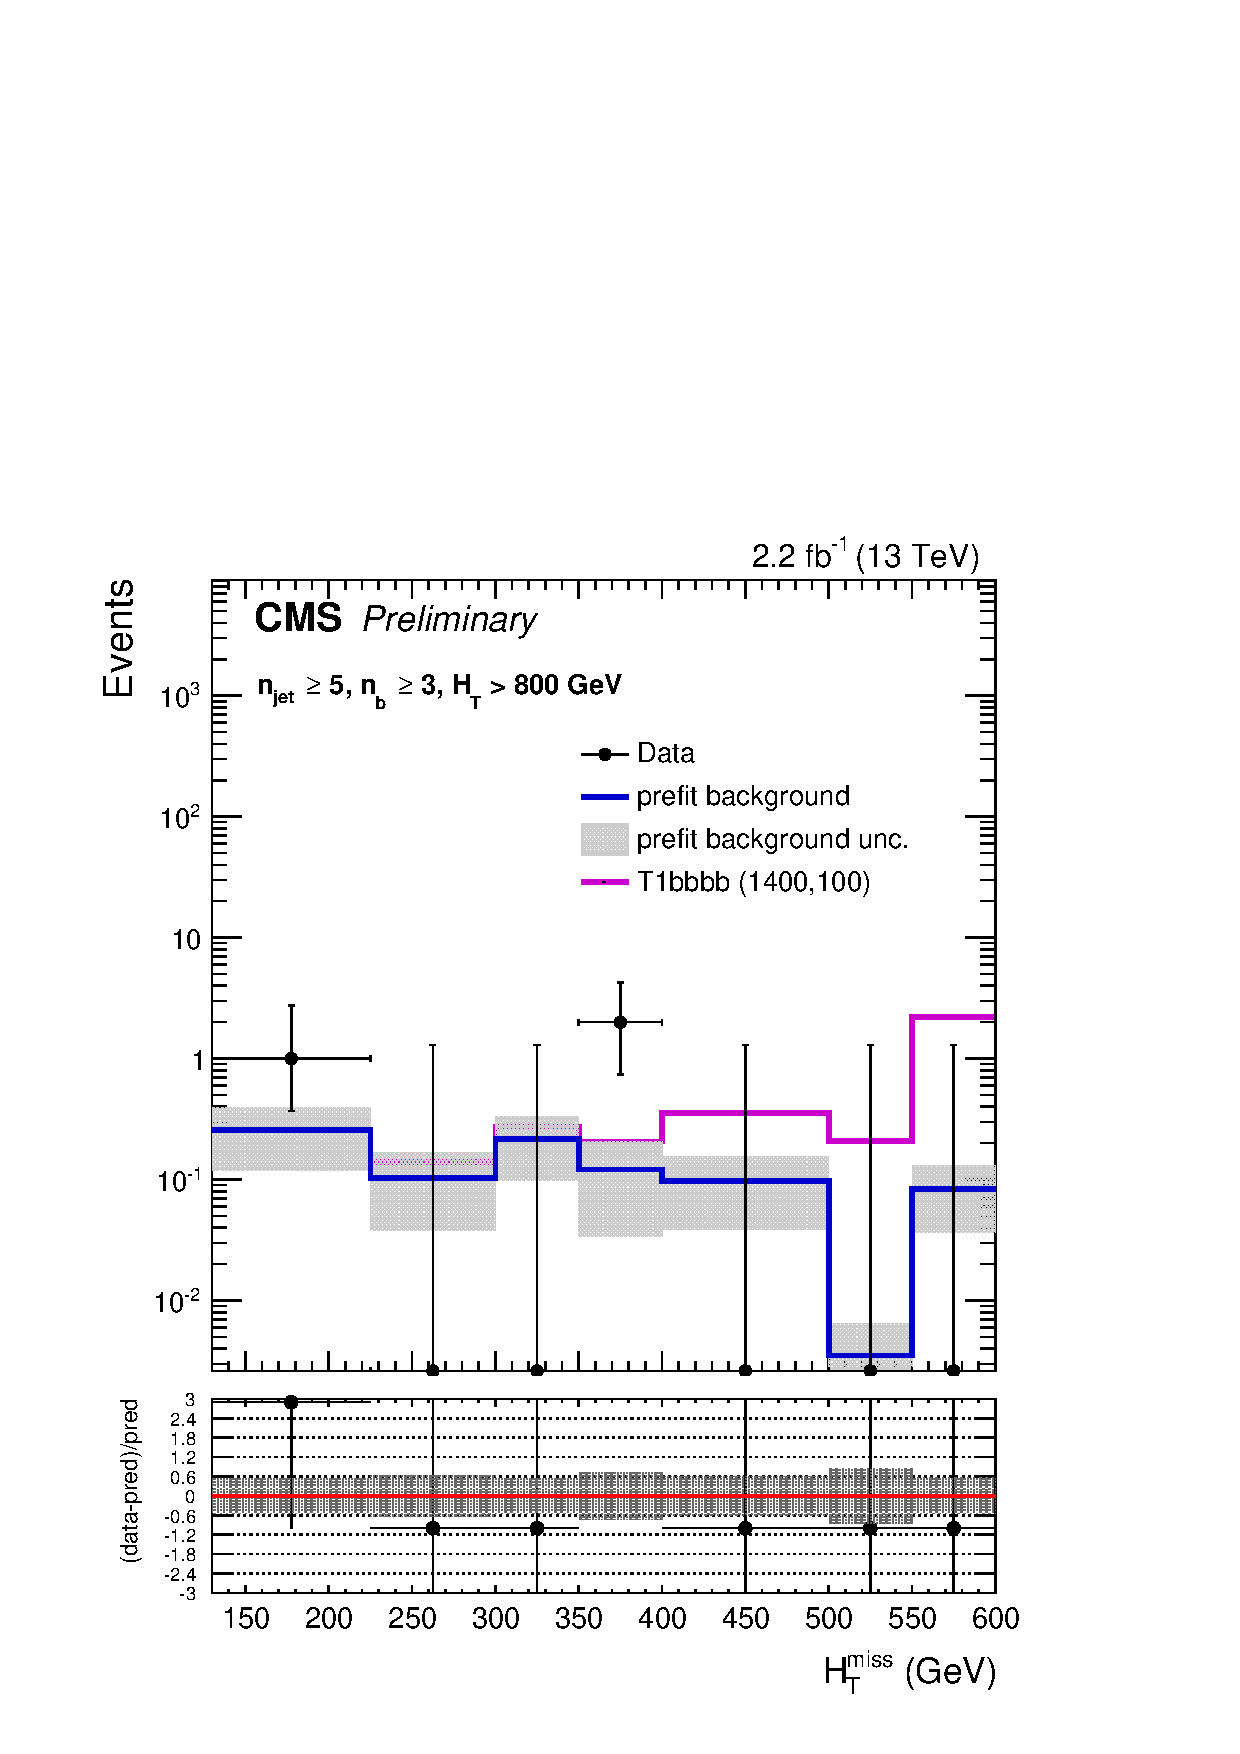
\includegraphics[width=0.45\textwidth]{AN-15-004/trunk/figures/postFitResults/shapePlots/postFitShape_ge3b_ge5j_800_Inf_prefit} } ~~
%    \subfigure[$\njet = 4$, $\nb = 2$, $500 < \scalht < 600$ GeV]{ 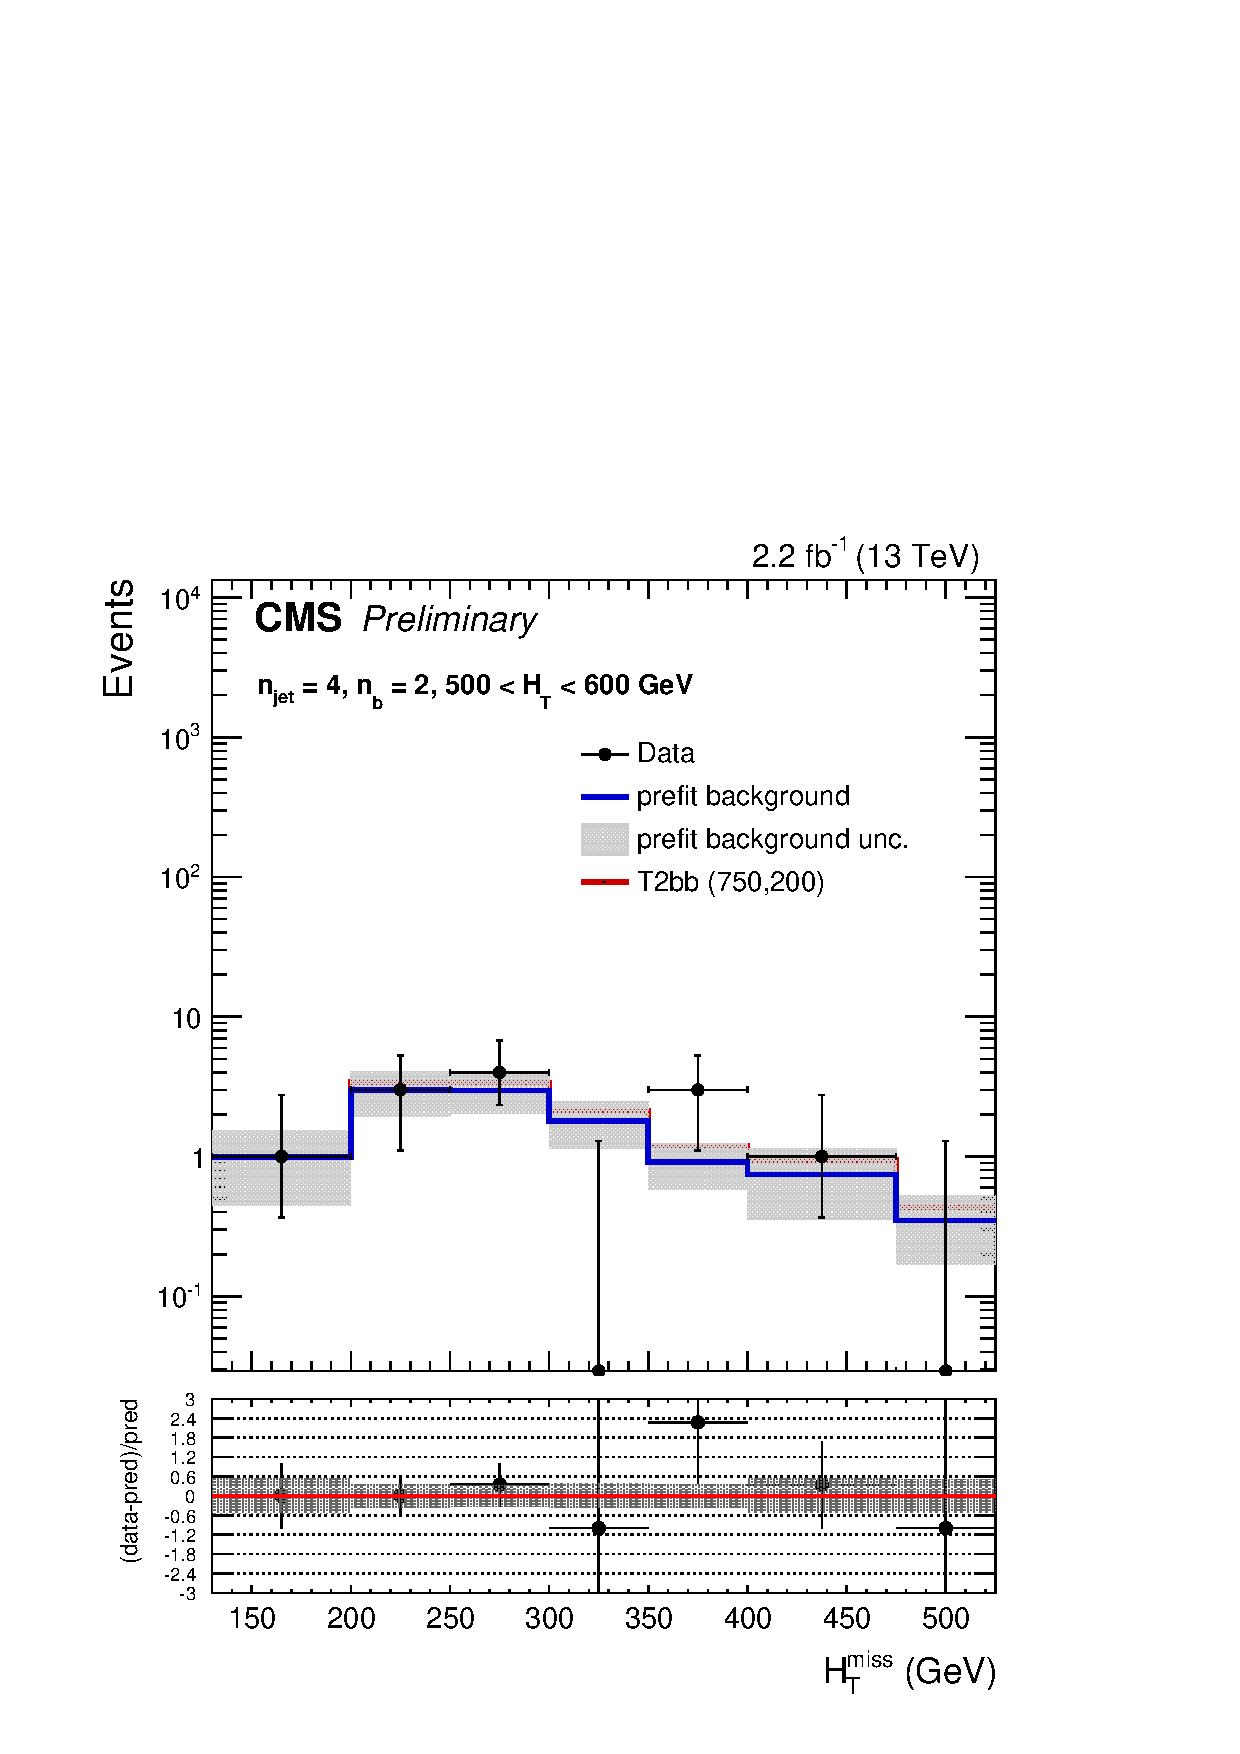
\includegraphics[width=0.45\textwidth]{AN-15-004/trunk/figures/postFitResults/shapePlots/postFitShape_eq2b_eq4j_500_600_prefit} } \\
%    \subfigure[$\njet \geq 5$, $\nb = 0$, $\scalht > 800$ GeV]   { 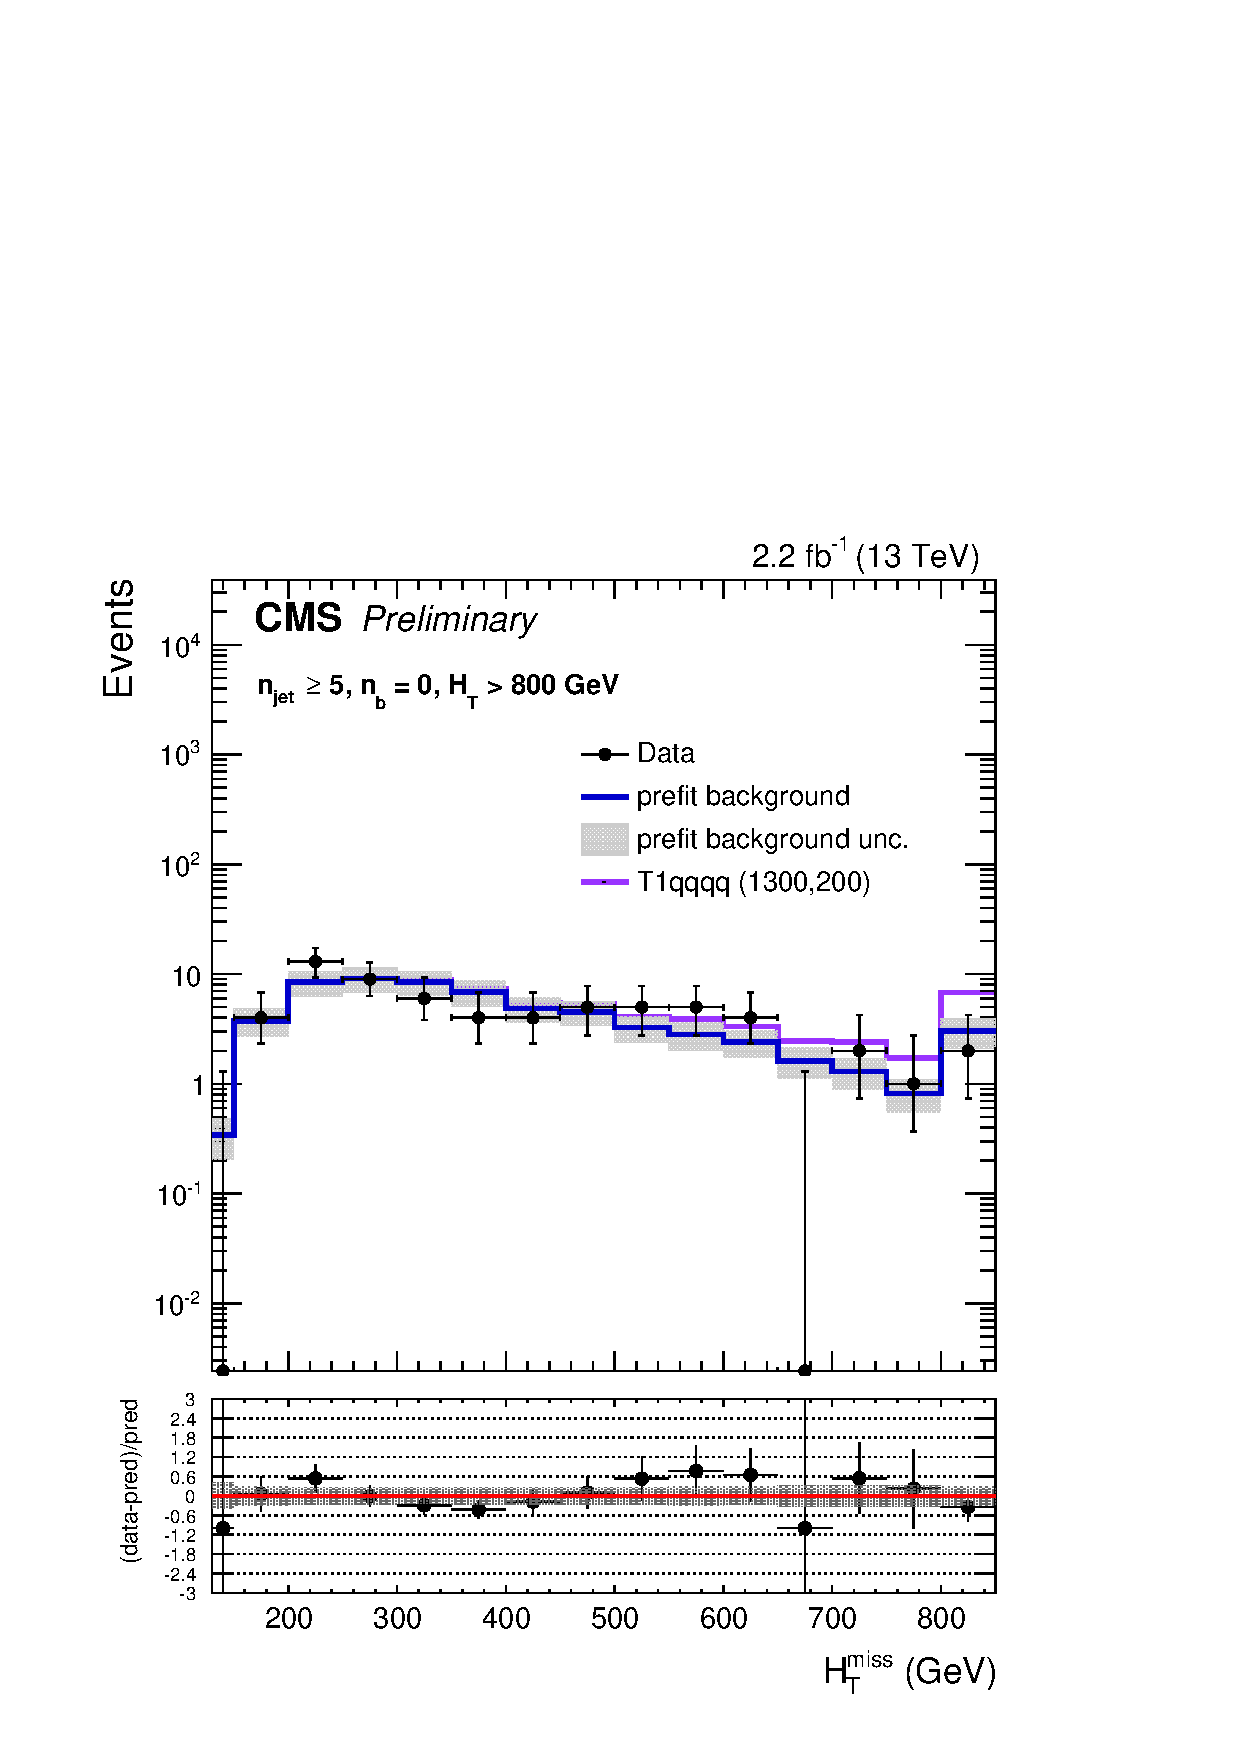
\includegraphics[width=0.45\textwidth]{AN-15-004/trunk/figures/postFitResults/shapePlots/postFitShape_eq0b_ge5j_800_Inf_prefit} } ~~
%    \subfigure[$\njet \geq 5$, $\nb = 1$, $600 < \scalht < 800$ GeV]{ 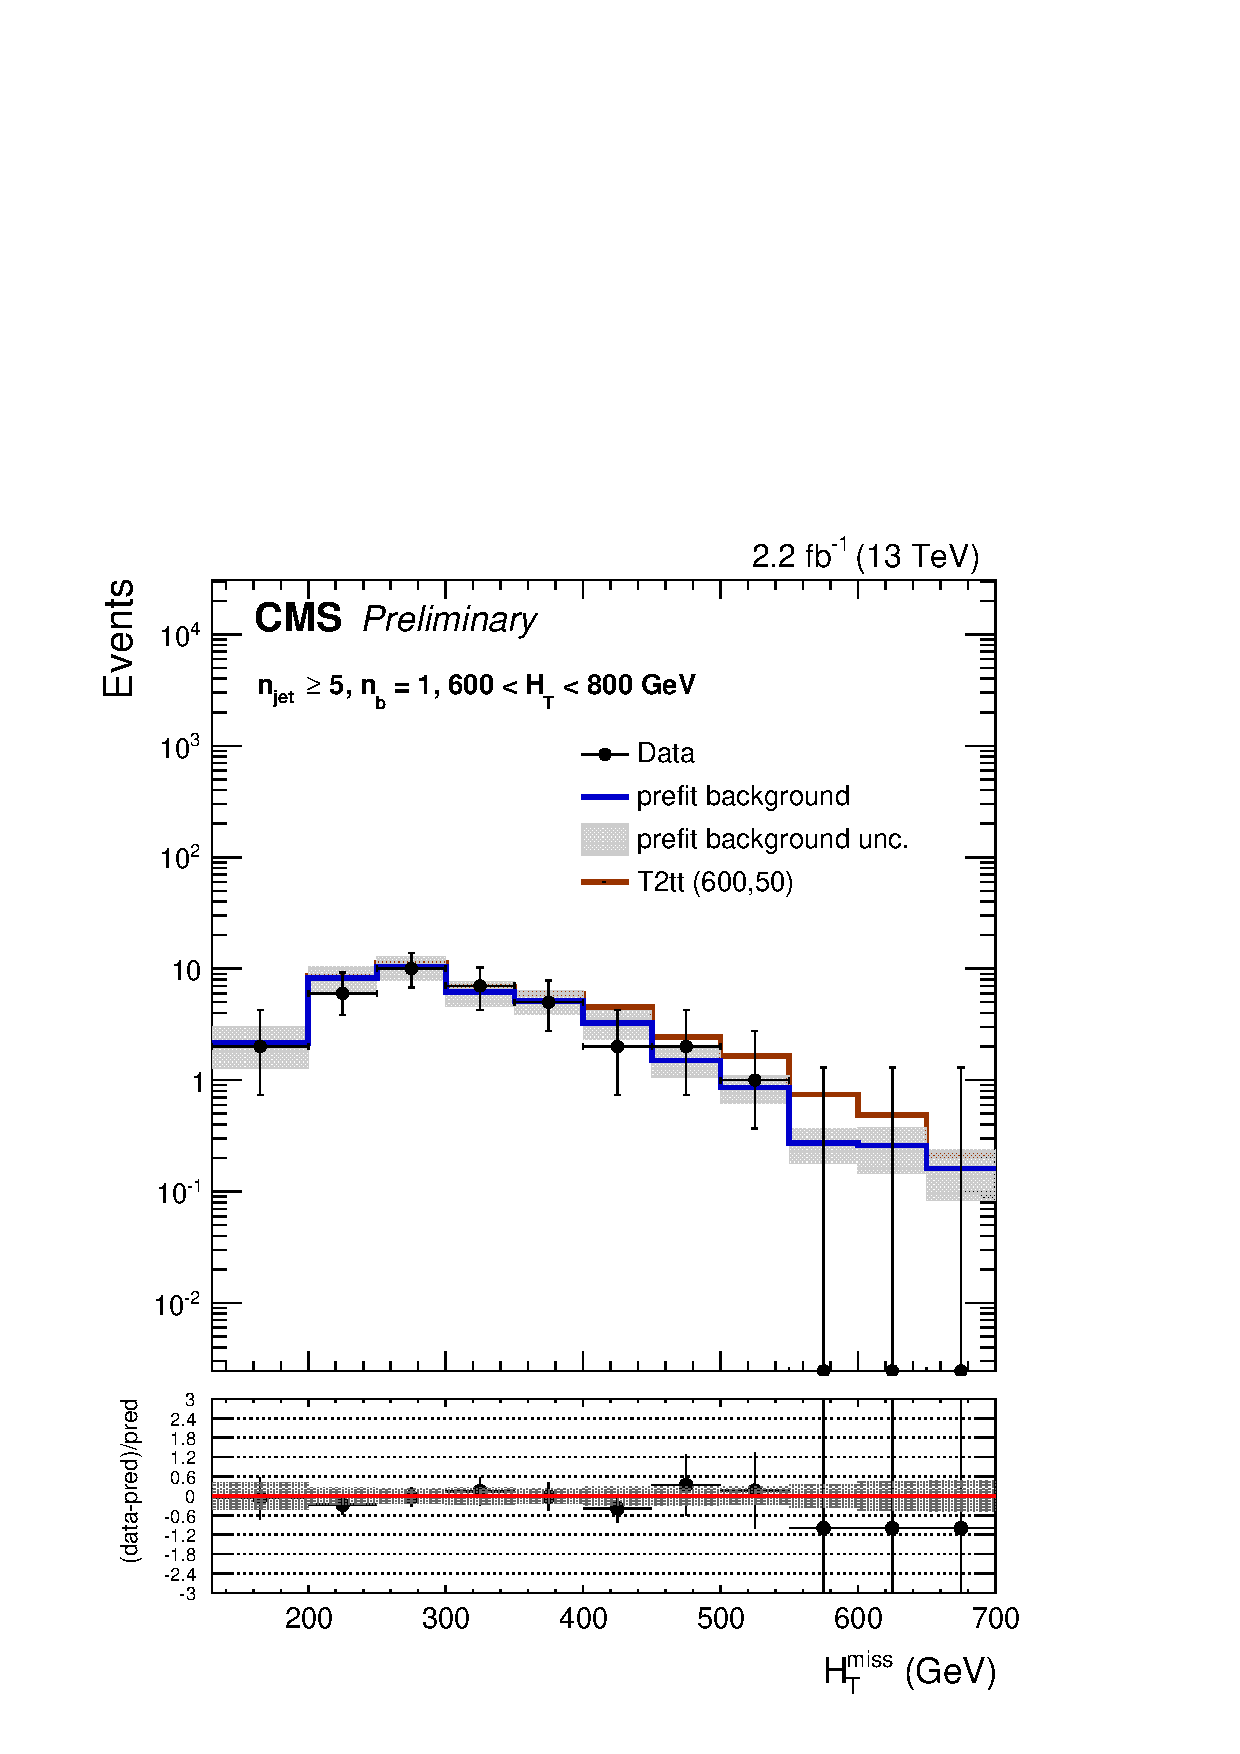
\includegraphics[width=0.45\textwidth]{AN-15-004/trunk/figures/postFitResults/shapePlots/postFitShape_eq1b_ge5j_600_800_prefit} } \\
%  \end{center}
%\end{figure}





\begin{table}[h!]
\tiny
\centering
\caption{Post fit Predictions and Data in the signal region for 2.1\ifb for monojet categories. All entries are non-zero but are truncated to one decimal place.\label{tab:predallqcdpost_sig_comb_mono}}
\begin{tabular}
{cccccccccc}
	\hline\hline
	&	& \multicolumn{8}{c}{\scalht (\gev)}\\ 
	&	 (\njet, \nb) & 200-250 & 250-300 & 300-350 & 350-400 & 400-500 & 500-600 & 600-800 & 800-$\infty$ \\ [0.8ex] 
\hline
	Data & (1, 0) & 11433 & 3758 & 1375 & 635 & 447 & 115 & 49 & -- \\[0.5ex] 
	SM & (1, 0) & $11410.9^{+ 115.4 }_{- 115.4 }$ & $3752.7^{+ 67.9 }_{- 67.9 }$ & $1368.0^{+ 35.7 }_{- 35.7 }$ & $627.3^{+ 22.7 }_{- 22.7 }$ & $442.4^{+ 22.3 }_{- 22.3 }$ & $115.7^{+ 9.5 }_{- 9.5 }$ & $49.1^{+ 6.6 }_{- 6.6 }$ & -- \\[0.5ex] 
	Ttw & (1, 0) & $4593.7^{+ 297.2 }_{- 297.2 }$ & $1372.7^{+ 129.8 }_{- 129.8 }$ & $442.5^{+ 35.4 }_{- 35.4 }$ & $169.4^{+ 26.0 }_{- 26.0 }$ & $120.8^{+ 21.4 }_{- 21.4 }$ & $26.2^{+ 5.5 }_{- 5.5 }$ & $11.2^{+ 4.8 }_{- 4.8 }$ & -- \\[0.5ex] 
	Zinv & (1, 0) & $6776.5^{+ 308.0 }_{- 308.0 }$ & $2380.0^{+ 132.7 }_{- 132.7 }$ & $925.3^{+ 46.0 }_{- 46.0 }$ & $457.9^{+ 33.3 }_{- 33.3 }$ & $320.6^{+ 27.5 }_{- 27.5 }$ & $89.5^{+ 10.2 }_{- 10.2 }$ & $37.9^{+ 7.3 }_{- 7.3 }$ & -- \\[0.5ex] 
	QCD & (1, 0) & $42.7^{+ 89.8 }_{- 42.7 }$ & $0.0^{+ 18.2 }_{- 0.0 }$ & $0.2^{+ 0.6 }_{- 0.2 }$ & $0.0^{+ 0.1 }_{- 0.0 }$ & $1.1^{+ 2.7 }_{- 1.1 }$ & $0.0^{+ 0.2 }_{- 0.0 }$ & $0.0^{+ 0.1 }_{- 0.0 }$ & -- \\[0.5ex] 
	Data & (1, 1) & 410 & 139 & 51 & 25 & 23 & 5 & -- & -- \\[0.5ex] 
	SM & (1, 1) & $415.9^{+ 17.3 }_{- 17.3 }$ & $140.2^{+ 10.2 }_{- 10.2 }$ & $51.6^{+ 6.0 }_{- 6.0 }$ & $23.2^{+ 4.4 }_{- 4.4 }$ & $19.8^{+ 3.2 }_{- 3.2 }$ & $4.4^{+ 1.5 }_{- 1.5 }$ & -- & -- \\[0.5ex] 
	Ttw & (1, 1) & $138.7^{+ 10.9 }_{- 10.9 }$ & $41.5^{+ 5.9 }_{- 5.9 }$ & $14.3^{+ 2.0 }_{- 2.0 }$ & $5.9^{+ 1.5 }_{- 1.5 }$ & $6.2^{+ 1.4 }_{- 1.4 }$ & $0.9^{+ 0.5 }_{- 0.5 }$ & -- & -- \\[0.5ex] 
	Zinv & (1, 1) & $275.5^{+ 16.3 }_{- 16.3 }$ & $98.6^{+ 8.8 }_{- 8.8 }$ & $37.3^{+ 4.6 }_{- 4.6 }$ & $17.3^{+ 3.6 }_{- 3.6 }$ & $13.5^{+ 2.7 }_{- 2.7 }$ & $3.5^{+ 1.3 }_{- 1.3 }$ & -- & -- \\[0.5ex] 
	QCD & (1, 1) & $1.6^{+ 3.3 }_{- 1.6 }$ & $0.0^{+ 0.7 }_{- 0.0 }$ & $0.0^{+ 0.0 }_{- 0.0 }$ & $0.0^{+ 0.0 }_{- 0.0 }$ & $0.0^{+ 0.1 }_{- 0.0 }$ & $0.0^{+ 0.0 }_{- 0.0 }$ & -- & -- \\[0.5ex] 
	\hline
	\hline
\end{tabular}
\end{table}


\begin{table}[h!]
\tiny
\centering
\caption{Post fit Predictions and Data in the signal region for 2.6\ifb for symmetric categories. All entries are non-zero but are truncated to one decimal place.\label{tab:predallqcdpost_sig_comb_sym}}
\scalebox{0.85}{\begin{tabular}{cccccccccc}
	\hline\hline
	&	& \multicolumn{8}{c}{\scalht (\gev)}\\ 
	&	 (\njet, \nb) & 200-250 & 250-300 & 300-350 & 350-400 & 400-500 & 500-600 & 600-800 & 800-$\infty$ \\ [0.8ex] 
\hline
	Data & (2, 0) & 1366 & 1350 & 911 & 521 & 452 & 131 & 88 & 76 \\[0.5ex] 
	SM & (2, 0) & $1369.6\pm 50.0$ & $1357.5\pm 45.3$ & $879.3\pm 27.4$ & $502.2\pm 25.1$ & $449.3\pm 15.0$ & $121.0\pm 6.4$ & $68.9\pm 3.6$ & $73.5\pm 6.0$ \\[0.5ex] 
	Ttw & (2, 0) & $628.9\pm 34.3$ & $604.0\pm 23.0$ & $372.6\pm 10.9$ & $194.0\pm 8.1$ & $163.2\pm 5.8$ & $39.7\pm 1.9$ & $20.1\pm 1.0$ & $22.7\pm 1.9$ \\[0.5ex] 
	Zinv & (2, 0) & $634.7\pm 35.2$ & $701.2\pm 26.9$ & $492.3\pm 14.9$ & $280.9\pm 11.8$ & $279.0\pm 9.7$ & $78.6\pm 3.8$ & $46.6\pm 2.4$ & $49.5\pm 4.1$ \\[0.5ex] 
	QCD & (2, 0) & $105.9\pm 80.1$ & $52.2\pm 48.1$ & $14.4\pm 17.0$ & $27.3\pm 27.4$ & $7.1\pm 6.5$ & $2.6\pm 3.5$ & $2.2\pm 2.2$ & $1.2\pm 1.0$ \\[0.5ex] 
	Data & (2, 1) & 116 & 110 & 74 & 25 & 26 & 6 & 3 & 4 \\[0.5ex] 
	SM & (2, 1) & $118.5\pm 10.8$ & $104.0\pm 8.8$ & $71.3\pm 5.9$ & $37.6\pm 4.3$ & $24.0\pm 2.4$ & $9.3\pm 1.2$ & $4.7\pm 0.8$ & $7.6\pm 1.2$ \\[0.5ex] 
	Ttw & (2, 1) & $67.5\pm 7.6$ & $53.3\pm 4.7$ & $26.9\pm 2.2$ & $13.1\pm 1.5$ & $6.5\pm 0.7$ & $2.1\pm 0.3$ & $0.9\pm 0.2$ & $1.3\pm 0.2$ \\[0.5ex] 
	Zinv & (2, 1) & $42.1\pm 4.7$ & $46.6\pm 4.1$ & $43.3\pm 3.6$ & $22.4\pm 2.5$ & $17.0\pm 1.7$ & $7.1\pm 0.9$ & $3.6\pm 0.6$ & $6.2\pm 1.0$ \\[0.5ex] 
	QCD & (2, 1) & $8.9\pm 6.8$ & $4.1\pm 3.8$ & $1.2\pm 1.4$ & $2.1\pm 2.1$ & $0.5\pm 0.5$ & $0.2\pm 0.3$ & $0.2\pm 0.2$ & $0.1\pm 0.1$ \\[0.5ex] 
	Data & (2, 2) & 5 & 6 & 8 & 0 & 1 & 0 & 0 & -- \\[0.5ex] 
	SM & (2, 2) & $5.5\pm 1.7$ & $7.6\pm 2.1$ & $5.0\pm 1.7$ & $1.9\pm 0.5$ & $0.8\pm 0.3$ & $0.5\pm 0.2$ & $0.1\pm 0.1$ & -- \\[0.5ex] 
	Ttw & (2, 2) & $2.0\pm 0.7$ & $2.8\pm 0.8$ & $2.1\pm 0.7$ & $0.5\pm 0.1$ & $0.0\pm 0.0$ & $0.1\pm 0.0$ & $0.0\pm 0.0$ & -- \\[0.5ex] 
	Zinv & (2, 2) & $3.0\pm 1.0$ & $4.4\pm 1.3$ & $2.9\pm 1.0$ & $1.3\pm 0.4$ & $0.7\pm 0.3$ & $0.4\pm 0.2$ & $0.1\pm 0.1$ & -- \\[0.5ex] 
	QCD & (2, 2) & $0.6\pm 0.4$ & $0.3\pm 0.3$ & $0.1\pm 0.1$ & $0.1\pm 0.1$ & $0.0\pm 0.0$ & $0.0\pm 0.0$ & $0.0\pm 0.0$ & -- \\[0.5ex] 
	Data & (3, 0) & 0 & 248 & 685 & 687 & 718 & 220 & 119 & 118 \\[0.5ex] 
	SM & (3, 0) & $1.4\pm 0.6$ & $246.3\pm 13.8$ & $668.8\pm 26.6$ & $691.6\pm 26.0$ & $721.3\pm 22.5$ & $227.5\pm 12.4$ & $132.6\pm 6.2$ & $112.0\pm 6.6$ \\[0.5ex] 
	Ttw & (3, 0) & $0.9\pm 0.4$ & $120.6\pm 7.2$ & $309.3\pm 16.7$ & $316.8\pm 12.6$ & $311.5\pm 9.9$ & $85.3\pm 4.8$ & $42.8\pm 2.1$ & $34.8\pm 1.8$ \\[0.5ex] 
	Zinv & (3, 0) & $0.5\pm 0.2$ & $122.2\pm 7.0$ & $319.7\pm 17.2$ & $342.9\pm 13.6$ & $392.3\pm 12.5$ & $131.7\pm 7.4$ & $89.0\pm 4.2$ & $72.7\pm 3.8$ \\[0.5ex] 
	QCD & (3, 0) & $0.0\pm 0.0$ & $3.5\pm 3.4$ & $39.7\pm 31.0$ & $31.8\pm 24.0$ & $17.6\pm 13.6$ & $10.5\pm 7.7$ & $0.9\pm 0.8$ & $4.4\pm 4.3$ \\[0.5ex] 
	Data & (3, 1) & 2 & 40 & 97 & 88 & 87 & 17 & 15 & 7 \\[0.5ex] 
	SM & (3, 1) & $0.5\pm 0.2$ & $45.1\pm 4.2$ & $114.4\pm 7.7$ & $102.8\pm 6.4$ & $100.3\pm 5.1$ & $25.8\pm 2.4$ & $14.6\pm 1.4$ & $12.0\pm 1.5$ \\[0.5ex] 
	Ttw & (3, 1) & $0.3\pm 0.1$ & $34.4\pm 3.2$ & $72.5\pm 4.6$ & $62.0\pm 3.8$ & $49.1\pm 2.7$ & $8.5\pm 0.8$ & $3.3\pm 0.3$ & $3.1\pm 0.4$ \\[0.5ex] 
	Zinv & (3, 1) & $0.2\pm 0.1$ & $10.0\pm 0.9$ & $35.6\pm 2.3$ & $36.1\pm 2.3$ & $48.9\pm 2.8$ & $16.2\pm 1.6$ & $11.2\pm 1.1$ & $8.4\pm 1.1$ \\[0.5ex] 
	QCD & (3, 1) & $0.0\pm 0.0$ & $0.7\pm 0.6$ & $6.3\pm 4.9$ & $4.7\pm 3.5$ & $2.3\pm 1.8$ & $1.2\pm 0.9$ & $0.1\pm 0.1$ & $0.5\pm 0.5$ \\[0.5ex] 
	Data & (3, 2) & -- & 5 & 14 & 15 & 18 & 1 & 1 & 2 \\[0.5ex] 
	SM & (3, 2) & -- & $4.6\pm 0.9$ & $15.4\pm 2.3$ & $16.1\pm 2.1$ & $14.8\pm 1.5$ & $2.7\pm 0.4$ & $1.4\pm 0.3$ & $0.5\pm 0.2$ \\[0.5ex] 
	Ttw & (3, 2) & -- & $3.1\pm 0.6$ & $10.5\pm 1.6$ & $11.0\pm 1.4$ & $10.5\pm 1.1$ & $0.9\pm 0.2$ & $0.3\pm 0.1$ & $0.1\pm 0.0$ \\[0.5ex] 
	Zinv & (3, 2) & -- & $1.5\pm 0.3$ & $3.8\pm 0.6$ & $4.4\pm 0.6$ & $4.0\pm 0.5$ & $1.7\pm 0.3$ & $1.1\pm 0.2$ & $0.4\pm 0.2$ \\[0.5ex] 
	QCD & (3, 2) & -- & $0.1\pm 0.1$ & $1.1\pm 0.8$ & $0.7\pm 0.5$ & $0.3\pm 0.3$ & $0.1\pm 0.1$ & $0.0\pm 0.0$ & $0.0\pm 0.0$ \\[0.5ex] 
	Data & (3, $\ge3$) & -- & 0 & -- & 0 & 0 & -- & -- & -- \\[0.5ex] 
	SM & (3, $\ge3$) & -- & $0.1\pm 0.1$ & -- & $0.3\pm 0.3$ & $0.1\pm 0.1$ & -- & -- & -- \\[0.5ex] 
	Ttw & (3, $\ge3$) & -- & $0.1\pm 0.1$ & -- & $0.2\pm 0.2$ & $0.1\pm 0.1$ & -- & -- & -- \\[0.5ex] 
	Zinv & (3, $\ge3$) & -- & $0.0\pm 0.0$ & -- & $0.1\pm 0.1$ & $0.0\pm 0.0$ & -- & -- & -- \\[0.5ex] 
	QCD & (3, $\ge3$) & -- & $0.0\pm 0.0$ & -- & $0.0\pm 0.0$ & $0.0\pm 0.0$ & -- & -- & -- \\[0.5ex] 
	Data & (4, 0) & -- & 3 & 74 & 272 & 511 & 208 & 135 & 82 \\[0.5ex] 
	SM & (4, 0) & -- & $1.5\pm 0.8$ & $84.1\pm 7.0$ & $254.8\pm 13.1$ & $495.1\pm 19.3$ & $197.9\pm 9.8$ & $126.9\pm 7.4$ & $86.2\pm 4.6$ \\[0.5ex] 
	Ttw & (4, 0) & -- & $1.1\pm 0.5$ & $47.3\pm 4.0$ & $134.7\pm 7.2$ & $224.6\pm 9.4$ & $88.2\pm 4.3$ & $45.6\pm 2.3$ & $29.8\pm 1.6$ \\[0.5ex] 
	Zinv & (4, 0) & -- & $0.5\pm 0.3$ & $36.7\pm 3.1$ & $115.9\pm 6.2$ & $232.1\pm 9.8$ & $106.7\pm 5.1$ & $76.1\pm 3.7$ & $55.1\pm 2.9$ \\[0.5ex] 
	QCD & (4, 0) & -- & $0.0\pm 0.0$ & $0.1\pm 0.1$ & $4.2\pm 4.4$ & $38.5\pm 21.4$ & $3.0\pm 2.8$ & $5.2\pm 5.5$ & $1.3\pm 1.3$ \\[0.5ex] 
	Data & (4, 1) & -- & 0 & 27 & 87 & 127 & 36 & 23 & 21 \\[0.5ex] 
	SM & (4, 1) & -- & $0.6\pm 0.5$ & $31.3\pm 3.8$ & $80.3\pm 5.5$ & $137.5\pm 6.9$ & $48.3\pm 3.4$ & $22.8\pm 2.4$ & $17.9\pm 1.8$ \\[0.5ex] 
	Ttw & (4, 1) & -- & $0.5\pm 0.5$ & $24.6\pm 3.0$ & $62.1\pm 4.3$ & $89.2\pm 4.4$ & $27.7\pm 2.0$ & $9.0\pm 1.0$ & $5.9\pm 0.6$ \\[0.5ex] 
	Zinv & (4, 1) & -- & $0.0\pm 0.0$ & $6.7\pm 0.8$ & $16.9\pm 1.2$ & $38.5\pm 2.1$ & $20.0\pm 1.5$ & $12.9\pm 1.4$ & $11.7\pm 1.2$ \\[0.5ex] 
	QCD & (4, 1) & -- & $0.0\pm 0.0$ & $0.0\pm 0.0$ & $1.3\pm 1.4$ & $9.8\pm 5.5$ & $0.6\pm 0.6$ & $0.9\pm 1.0$ & $0.2\pm 0.2$ \\[0.5ex] 
	Data & (4, 2) & -- & -- & 5 & 23 & 40 & 10 & 1 & 3 \\[0.5ex] 
	SM & (4, 2) & -- & -- & $8.4\pm 1.8$ & $22.3\pm 2.8$ & $35.4\pm 2.8$ & $12.0\pm 1.4$ & $4.7\pm 0.7$ & $1.8\pm 0.4$ \\[0.5ex] 
	Ttw & (4, 2) & -- & -- & $7.2\pm 1.5$ & $19.8\pm 2.6$ & $26.1\pm 2.2$ & $9.0\pm 1.1$ & $2.4\pm 0.3$ & $0.6\pm 0.1$ \\[0.5ex] 
	Zinv & (4, 2) & -- & -- & $1.2\pm 0.3$ & $2.1\pm 0.3$ & $6.5\pm 0.6$ & $2.9\pm 0.3$ & $2.1\pm 0.3$ & $1.2\pm 0.3$ \\[0.5ex] 
	QCD & (4, 2) & -- & -- & $0.0\pm 0.0$ & $0.4\pm 0.4$ & $2.8\pm 1.6$ & $0.1\pm 0.1$ & $0.2\pm 0.2$ & $0.0\pm 0.0$ \\[0.5ex] 
	Data & (4, $\ge3$) & -- & -- & -- & 0 & 1 & 0 & 0 & 0 \\[0.5ex] 
	SM & (4, $\ge3$) & -- & -- & -- & $0.7\pm 0.4$ & $1.7\pm 0.6$ & $0.5\pm 0.2$ & $0.1\pm 0.1$ & $0.1\pm 0.1$ \\[0.5ex] 
	Ttw & (4, $\ge3$) & -- & -- & -- & $0.5\pm 0.3$ & $1.2\pm 0.5$ & $0.3\pm 0.1$ & $0.1\pm 0.0$ & $0.0\pm 0.0$ \\[0.5ex] 
	Zinv & (4, $\ge3$) & -- & -- & -- & $0.1\pm 0.1$ & $0.3\pm 0.1$ & $0.1\pm 0.1$ & $0.0\pm 0.0$ & $0.1\pm 0.0$ \\[0.5ex] 
	QCD & (4, $\ge3$) & -- & -- & -- & $0.0\pm 0.0$ & $0.2\pm 0.1$ & $0.0\pm 0.0$ & $0.0\pm 0.0$ & $0.0\pm 0.0$ \\[0.5ex] 
	Data & ($\ge5$, 0) & -- & -- & -- & 18 & 139 & 114 & 84 & 99 \\[0.5ex] 
	SM & ($\ge5$, 0) & -- & -- & -- & $11.8\pm 2.3$ & $134.8\pm 8.0$ & $108.2\pm 7.8$ & $101.2\pm 5.3$ & $88.1\pm 7.9$ \\[0.5ex] 
	Ttw & ($\ge5$, 0) & -- & -- & -- & $6.6\pm 1.3$ & $77.6\pm 4.7$ & $54.0\pm 3.7$ & $47.0\pm 2.5$ & $33.9\pm 2.0$ \\[0.5ex] 
	Zinv & ($\ge5$, 0) & -- & -- & -- & $5.2\pm 1.0$ & $53.5\pm 3.3$ & $48.6\pm 3.3$ & $53.0\pm 2.8$ & $47.1\pm 2.8$ \\[0.5ex] 
	QCD & ($\ge5$, 0) & -- & -- & -- & $0.0\pm 0.0$ & $3.8\pm 2.8$ & $5.7\pm 6.5$ & $1.2\pm 1.4$ & $7.2\pm 7.9$ \\[0.5ex] 
	Data & ($\ge5$, 1) & -- & -- & -- & 2 & 63 & 53 & 36 & 26 \\[0.5ex] 
	SM & ($\ge5$, 1) & -- & -- & -- & $6.1\pm 1.6$ & $66.1\pm 4.7$ & $49.6\pm 3.6$ & $36.4\pm 2.6$ & $27.2\pm 2.8$ \\[0.5ex] 
	Ttw & ($\ge5$, 1) & -- & -- & -- & $5.2\pm 1.3$ & $53.8\pm 4.0$ & $37.0\pm 2.5$ & $23.5\pm 1.7$ & $14.3\pm 1.4$ \\[0.5ex] 
	Zinv & ($\ge5$, 1) & -- & -- & -- & $0.9\pm 0.2$ & $10.4\pm 0.8$ & $10.2\pm 0.7$ & $12.5\pm 0.9$ & $10.8\pm 1.2$ \\[0.5ex] 
	QCD & ($\ge5$, 1) & -- & -- & -- & $0.0\pm 0.0$ & $1.8\pm 1.3$ & $2.3\pm 2.6$ & $0.4\pm 0.4$ & $2.1\pm 2.3$ \\[0.5ex] 
	Data & ($\ge5$, 2) & -- & -- & -- & 3 & 19 & 19 & 6 & 6 \\[0.5ex] 
	SM & ($\ge5$, 2) & -- & -- & -- & $3.0\pm 0.9$ & $23.9\pm 2.6$ & $16.7\pm 1.8$ & $10.7\pm 1.2$ & $8.9\pm 1.1$ \\[0.5ex] 
	Ttw & ($\ge5$, 2) & -- & -- & -- & $2.9\pm 0.9$ & $21.3\pm 2.3$ & $13.9\pm 1.5$ & $8.6\pm 1.0$ & $5.9\pm 0.7$ \\[0.5ex] 
	Zinv & ($\ge5$, 2) & -- & -- & -- & $0.1\pm 0.0$ & $1.8\pm 0.2$ & $1.9\pm 0.2$ & $1.9\pm 0.2$ & $2.3\pm 0.3$ \\[0.5ex] 
	QCD & ($\ge5$, 2) & -- & -- & -- & $0.0\pm 0.0$ & $0.8\pm 0.6$ & $0.9\pm 1.0$ & $0.1\pm 0.2$ & $0.6\pm 0.7$ \\[0.5ex] 
	Data & ($\ge5$, $\ge3$) & -- & -- & -- & -- & 0 & 0 & 1 & 1 \\[0.5ex] 
	SM & ($\ge5$, $\ge3$) & -- & -- & -- & -- & $1.4\pm 0.6$ & $1.1\pm 0.4$ & $1.2\pm 0.3$ & $0.8\pm 0.3$ \\[0.5ex] 
	Ttw & ($\ge5$, $\ge3$) & -- & -- & -- & -- & $1.2\pm 0.5$ & $1.0\pm 0.3$ & $0.7\pm 0.2$ & $0.5\pm 0.2$ \\[0.5ex] 
	Zinv & ($\ge5$, $\ge3$) & -- & -- & -- & -- & $0.2\pm 0.1$ & $0.1\pm 0.0$ & $0.4\pm 0.1$ & $0.3\pm 0.1$ \\[0.5ex] 
	QCD & ($\ge5$, $\ge3$) & -- & -- & -- & -- & $0.0\pm 0.0$ & $0.1\pm 0.1$ & $0.0\pm 0.0$ & $0.1\pm 0.1$ \\[0.5ex] 
	\hline
	\hline
\end{tabular}}
\end{table}


\begin{table}[h!]
\tiny
\centering
\caption{Post fit Predictions and Data in the signal region for 12.9\ifb for asymmetric categories. The letter ``a'' in jet \eg ``2a''  indicates the asymmetric jet bins. All entries are non-zero but are truncated to one decimal place.\label{tab:predallqcdpost_sig_comb_asym}}
\scalebox{0.85}{\begin{tabular}{cccccccccc}
	\hline\hline
	&	& \multicolumn{8}{c}{\scalht (\gev)}\\ 
	&	 (\njet, \nb) & 200-250 & 250-300 & 300-350 & 350-400 & 400-500 & 500-600 & 600-800 & 800-$\infty$ \\ [0.8ex] 
\hline
	Data & (2a, 0) & 29737 & 8553 & 3157 & 1189 & 708 & 166 & 124 & -- \\[0.5ex] 
	SM & (2a, 0) & $29730.5\pm 156.5$ & $8642.8\pm 73.2$ & $3141.5\pm 40.4$ & $1180.1\pm 24.4$ & $763.7\pm 14.5$ & $169.3\pm 6.2$ & $122.5\pm 6.1$ & -- \\[0.5ex] 
	Ttw & (2a, 0) & $14949.1\pm 87.6$ & $3991.1\pm 34.0$ & $1311.6\pm 16.9$ & $452.7\pm 9.4$ & $254.4\pm 4.8$ & $43.3\pm 1.6$ & $34.1\pm 2.1$ & -- \\[0.5ex] 
	Zinv & (2a, 0) & $14636.7\pm 82.4$ & $4635.0\pm 38.8$ & $1825.2\pm 23.6$ & $727.2\pm 15.1$ & $508.2\pm 9.6$ & $125.9\pm 4.6$ & $88.3\pm 4.4$ & -- \\[0.5ex] 
	QCD & (2a, 0) & $144.6\pm 95.0$ & $16.7\pm 10.9$ & $4.7\pm 4.2$ & $0.2\pm 0.2$ & $1.0\pm 1.0$ & $0.0\pm 0.0$ & $0.0\pm 0.0$ & -- \\[0.5ex] 
	Data & (2a, 1) & 3227 & 944 & 292 & 98 & 77 & 39 & -- & -- \\[0.5ex] 
	SM & (2a, 1) & $3286.5\pm 39.8$ & $890.9\pm 17.5$ & $279.5\pm 8.6$ & $115.9\pm 5.4$ & $76.2\pm 4.0$ & $36.0\pm 3.8$ & -- & -- \\[0.5ex] 
	Ttw & (2a, 1) & $2024.9\pm 25.6$ & $481.7\pm 9.5$ & $126.2\pm 3.9$ & $49.5\pm 2.3$ & $26.5\pm 1.4$ & $11.3\pm 1.3$ & -- & -- \\[0.5ex] 
	Zinv & (2a, 1) & $1244.6\pm 15.7$ & $407.5\pm 8.3$ & $152.8\pm 4.8$ & $66.3\pm 3.1$ & $49.6\pm 2.6$ & $24.6\pm 2.6$ & -- & -- \\[0.5ex] 
	QCD & (2a, 1) & $17.0\pm 11.2$ & $1.7\pm 1.1$ & $0.4\pm 0.4$ & $0.0\pm 0.0$ & $0.1\pm 0.1$ & $0.0\pm 0.0$ & -- & -- \\[0.5ex] 
	Data & (2a, 2) & 225 & 50 & 12 & 6 & 6 & -- & -- & -- \\[0.5ex] 
	SM & (2a, 2) & $214.8\pm 8.8$ & $56.9\pm 3.8$ & $14.8\pm 1.5$ & $3.8\pm 0.6$ & $6.3\pm 1.4$ & -- & -- & -- \\[0.5ex] 
	Ttw & (2a, 2) & $126.0\pm 5.3$ & $33.1\pm 2.2$ & $6.0\pm 0.6$ & $1.2\pm 0.2$ & $2.6\pm 0.6$ & -- & -- & -- \\[0.5ex] 
	Zinv & (2a, 2) & $87.8\pm 3.6$ & $23.6\pm 1.6$ & $8.8\pm 0.9$ & $2.6\pm 0.4$ & $3.7\pm 0.8$ & -- & -- & -- \\[0.5ex] 
	QCD & (2a, 2) & $1.1\pm 0.7$ & $0.1\pm 0.1$ & $0.0\pm 0.0$ & $0.0\pm 0.0$ & $0.0\pm 0.0$ & -- & -- & -- \\[0.5ex] 
	Data & (3a, 0) & 7843 & 7827 & 3798 & 1168 & 530 & 71 & 44 & -- \\[0.5ex] 
	SM & (3a, 0) & $7837.6\pm 72.9$ & $7758.6\pm 73.8$ & $3794.0\pm 59.9$ & $1223.1\pm 23.1$ & $512.7\pm 11.0$ & $78.4\pm 3.4$ & $48.4\pm 3.9$ & -- \\[0.5ex] 
	Ttw & (3a, 0) & $4383.8\pm 41.8$ & $4211.3\pm 41.8$ & $1899.8\pm 31.8$ & $560.3\pm 10.5$ & $209.3\pm 4.6$ & $24.1\pm 1.1$ & $15.1\pm 1.3$ & -- \\[0.5ex] 
	Zinv & (3a, 0) & $3422.7\pm 32.2$ & $3529.5\pm 34.7$ & $1778.6\pm 30.2$ & $662.4\pm 12.6$ & $303.4\pm 6.7$ & $54.3\pm 2.4$ & $33.2\pm 2.7$ & -- \\[0.5ex] 
	QCD & (3a, 0) & $31.2\pm 9.1$ & $17.9\pm 12.6$ & $115.6\pm 45.9$ & $0.4\pm 0.4$ & $0.0\pm 0.0$ & $0.0\pm 0.0$ & $0.0\pm 0.0$ & -- \\[0.5ex] 
	Data & (3a, 1) & 1922 & 1901 & 885 & 237 & 79 & 6 & 8 & -- \\[0.5ex] 
	SM & (3a, 1) & $1920.3\pm 27.5$ & $1879.9\pm 30.3$ & $897.2\pm 18.8$ & $237.6\pm 7.8$ & $100.3\pm 4.3$ & $8.1\pm 1.0$ & $9.6\pm 1.2$ & -- \\[0.5ex] 
	Ttw & (3a, 1) & $1483.4\pm 21.5$ & $1431.0\pm 23.0$ & $637.1\pm 14.9$ & $150.8\pm 5.0$ & $52.1\pm 2.2$ & $2.0\pm 0.2$ & $3.5\pm 0.4$ & -- \\[0.5ex] 
	Zinv & (3a, 1) & $429.5\pm 6.5$ & $444.6\pm 8.3$ & $232.5\pm 5.7$ & $86.7\pm 2.9$ & $48.1\pm 2.1$ & $6.1\pm 0.7$ & $6.1\pm 0.8$ & -- \\[0.5ex] 
	QCD & (3a, 1) & $7.4\pm 2.1$ & $4.4\pm 3.1$ & $27.5\pm 10.9$ & $0.1\pm 0.1$ & $0.0\pm 0.0$ & $0.0\pm 0.0$ & $0.0\pm 0.0$ & -- \\[0.5ex] 
	Data & (3a, 2) & 349 & 325 & 166 & 40 & 11 & 0 & -- & -- \\[0.5ex] 
	SM & (3a, 2) & $337.4\pm 10.0$ & $338.1\pm 10.2$ & $165.0\pm 6.8$ & $40.1\pm 2.8$ & $14.2\pm 1.3$ & $2.4\pm 0.4$ & -- & -- \\[0.5ex] 
	Ttw & (3a, 2) & $282.3\pm 8.5$ & $283.8\pm 8.5$ & $134.3\pm 5.8$ & $31.5\pm 2.2$ & $7.3\pm 0.7$ & $0.1\pm 0.0$ & -- & -- \\[0.5ex] 
	Zinv & (3a, 2) & $53.7\pm 1.6$ & $53.6\pm 1.6$ & $25.9\pm 1.1$ & $8.6\pm 0.6$ & $6.8\pm 0.6$ & $2.3\pm 0.4$ & -- & -- \\[0.5ex] 
	QCD & (3a, 2) & $1.3\pm 0.4$ & $0.8\pm 0.6$ & $4.9\pm 2.0$ & $0.0\pm 0.0$ & $0.0\pm 0.0$ & $0.0\pm 0.0$ & -- & -- \\[0.5ex] 
	Data & (3a, $\ge3$) & 7 & 16 & 8 & -- & -- & -- & -- & -- \\[0.5ex] 
	SM & (3a, $\ge3$) & $8.0\pm 1.4$ & $11.8\pm 1.5$ & $6.9\pm 1.3$ & -- & -- & -- & -- & -- \\[0.5ex] 
	Ttw & (3a, $\ge3$) & $6.9\pm 1.2$ & $9.8\pm 1.2$ & $5.6\pm 1.1$ & -- & -- & -- & -- & -- \\[0.5ex] 
	Zinv & (3a, $\ge3$) & $1.1\pm 0.2$ & $1.9\pm 0.2$ & $1.0\pm 0.2$ & -- & -- & -- & -- & -- \\[0.5ex] 
	QCD & (3a, $\ge3$) & $0.0\pm 0.0$ & $0.0\pm 0.0$ & $0.2\pm 0.2$ & -- & -- & -- & -- & -- \\[0.5ex] 
	Data & (4a, 0) & 30 & 770 & 1953 & 1267 & 704 & 68 & 24 & -- \\[0.5ex] 
	SM & (4a, 0) & $29.9\pm 3.0$ & $775.9\pm 17.6$ & $1981.2\pm 41.7$ & $1207.7\pm 26.2$ & $687.6\pm 16.1$ & $77.0\pm 5.7$ & $18.9\pm 1.8$ & -- \\[0.5ex] 
	Ttw & (4a, 0) & $17.8\pm 1.8$ & $446.7\pm 9.2$ & $1141.6\pm 23.7$ & $684.0\pm 15.1$ & $354.2\pm 8.4$ & $32.4\pm 2.4$ & $5.0\pm 0.6$ & -- \\[0.5ex] 
	Zinv & (4a, 0) & $12.1\pm 1.2$ & $320.7\pm 6.6$ & $770.2\pm 16.3$ & $522.0\pm 11.3$ & $333.3\pm 7.7$ & $44.6\pm 3.3$ & $13.9\pm 1.3$ & -- \\[0.5ex] 
	QCD & (4a, 0) & $0.0\pm 0.0$ & $8.4\pm 8.3$ & $69.5\pm 40.2$ & $1.7\pm 2.3$ & $0.1\pm 0.1$ & $0.0\pm 0.0$ & $0.0\pm 0.0$ & -- \\[0.5ex] 
	Data & (4a, 1) & 11 & 309 & 855 & 514 & 227 & 19 & 3 & -- \\[0.5ex] 
	SM & (4a, 1) & $10.0\pm 1.3$ & $318.3\pm 10.8$ & $859.1\pm 20.7$ & $496.7\pm 12.9$ & $245.3\pm 7.4$ & $23.9\pm 1.8$ & $5.0\pm 0.7$ & -- \\[0.5ex] 
	Ttw & (4a, 1) & $8.2\pm 1.0$ & $262.2\pm 8.2$ & $694.3\pm 14.4$ & $401.4\pm 10.5$ & $179.3\pm 5.5$ & $14.9\pm 1.1$ & $1.4\pm 0.2$ & -- \\[0.5ex] 
	Zinv & (4a, 1) & $1.8\pm 0.2$ & $52.7\pm 1.8$ & $134.8\pm 3.1$ & $94.6\pm 2.6$ & $65.9\pm 2.1$ & $8.9\pm 0.7$ & $3.6\pm 0.5$ & -- \\[0.5ex] 
	QCD & (4a, 1) & $0.0\pm 0.0$ & $3.5\pm 3.4$ & $30.0\pm 17.3$ & $0.7\pm 1.0$ & $0.0\pm 0.0$ & $0.0\pm 0.0$ & $0.0\pm 0.0$ & -- \\[0.5ex] 
	Data & (4a, 2) & 2 & 78 & 322 & 186 & 81 & 3 & 0 & -- \\[0.5ex] 
	SM & (4a, 2) & $1.6\pm 0.3$ & $87.3\pm 4.3$ & $302.3\pm 9.6$ & $171.2\pm 6.9$ & $84.6\pm 4.5$ & $4.8\pm 0.7$ & $0.6\pm 0.1$ & -- \\[0.5ex] 
	Ttw & (4a, 2) & $1.1\pm 0.2$ & $78.6\pm 3.9$ & $269.6\pm 9.1$ & $155.9\pm 6.3$ & $73.5\pm 3.9$ & $3.4\pm 0.5$ & $0.3\pm 0.1$ & -- \\[0.5ex] 
	Zinv & (4a, 2) & $0.5\pm 0.1$ & $7.7\pm 0.4$ & $22.5\pm 0.8$ & $15.0\pm 0.6$ & $11.1\pm 0.6$ & $1.4\pm 0.2$ & $0.4\pm 0.1$ & -- \\[0.5ex] 
	QCD & (4a, 2) & $0.0\pm 0.0$ & $1.0\pm 1.0$ & $10.2\pm 5.9$ & $0.2\pm 0.3$ & $0.0\pm 0.0$ & $0.0\pm 0.0$ & $0.0\pm 0.0$ & -- \\[0.5ex] 
	Data & (4a, $\ge3$) & -- & 3 & 16 & 14 & 9 & -- & -- & -- \\[0.5ex] 
	SM & (4a, $\ge3$) & -- & $6.5\pm 1.2$ & $20.7\pm 2.2$ & $14.5\pm 1.9$ & $6.8\pm 1.2$ & -- & -- & -- \\[0.5ex] 
	Ttw & (4a, $\ge3$) & -- & $6.1\pm 1.2$ & $18.8\pm 2.1$ & $13.9\pm 1.8$ & $6.5\pm 1.2$ & -- & -- & -- \\[0.5ex] 
	Zinv & (4a, $\ge3$) & -- & $0.3\pm 0.1$ & $1.0\pm 0.1$ & $0.6\pm 0.1$ & $0.3\pm 0.1$ & -- & -- & -- \\[0.5ex] 
	QCD & (4a, $\ge3$) & -- & $0.1\pm 0.1$ & $0.8\pm 0.4$ & $0.0\pm 0.0$ & $0.0\pm 0.0$ & -- & -- & -- \\[0.5ex] 
	Data & ($\ge5$a, 0) & -- & 6 & 166 & 451 & 528 & 95 & 26 & -- \\[0.5ex] 
	SM & ($\ge5$a, 0) & -- & $4.2\pm 1.1$ & $156.2\pm 8.6$ & $435.3\pm 13.4$ & $530.1\pm 15.8$ & $102.7\pm 5.4$ & $22.8\pm 1.9$ & -- \\[0.5ex] 
	Ttw & ($\ge5$a, 0) & -- & $3.0\pm 0.8$ & $104.0\pm 5.7$ & $297.3\pm 9.2$ & $339.0\pm 10.2$ & $55.0\pm 2.9$ & $7.3\pm 0.7$ & -- \\[0.5ex] 
	Zinv & ($\ge5$a, 0) & -- & $1.2\pm 0.3$ & $52.2\pm 2.8$ & $138.0\pm 4.2$ & $190.9\pm 5.6$ & $46.3\pm 2.5$ & $15.4\pm 1.3$ & -- \\[0.5ex] 
	QCD & ($\ge5$a, 0) & -- & $0.0\pm 0.0$ & $0.0\pm 0.0$ & $0.0\pm 0.0$ & $0.2\pm 0.2$ & $1.3\pm 1.0$ & $0.0\pm 0.0$ & -- \\[0.5ex] 
	Data & ($\ge5$a, 1) & -- & 2 & 114 & 268 & 373 & 62 & 12 & -- \\[0.5ex] 
	SM & ($\ge5$a, 1) & -- & $2.7\pm 0.7$ & $119.1\pm 6.9$ & $274.2\pm 10.7$ & $347.5\pm 11.4$ & $61.7\pm 4.1$ & $10.4\pm 1.2$ & -- \\[0.5ex] 
	Ttw & ($\ge5$a, 1) & -- & $2.2\pm 0.6$ & $107.2\pm 6.2$ & $247.5\pm 9.7$ & $306.0\pm 10.1$ & $50.1\pm 3.4$ & $8.0\pm 0.9$ & -- \\[0.5ex] 
	Zinv & ($\ge5$a, 1) & -- & $0.5\pm 0.1$ & $11.9\pm 0.7$ & $26.7\pm 1.1$ & $41.4\pm 1.4$ & $10.8\pm 0.8$ & $2.4\pm 0.3$ & -- \\[0.5ex] 
	QCD & ($\ge5$a, 1) & -- & $0.0\pm 0.0$ & $0.0\pm 0.0$ & $0.0\pm 0.0$ & $0.1\pm 0.1$ & $0.8\pm 0.6$ & $0.0\pm 0.0$ & -- \\[0.5ex] 
	Data & ($\ge5$a, 2) & -- & 1 & 45 & 138 & 162 & 34 & 3 & -- \\[0.5ex] 
	SM & ($\ge5$a, 2) & -- & $1.9\pm 0.7$ & $46.9\pm 3.8$ & $138.9\pm 7.2$ & $175.0\pm 7.9$ & $29.7\pm 2.3$ & $4.7\pm 0.6$ & -- \\[0.5ex] 
	Ttw & ($\ge5$a, 2) & -- & $1.9\pm 0.7$ & $45.2\pm 3.7$ & $133.8\pm 6.9$ & $167.0\pm 7.5$ & $27.3\pm 2.2$ & $4.3\pm 0.5$ & -- \\[0.5ex] 
	Zinv & ($\ge5$a, 2) & -- & $0.0\pm 0.0$ & $1.7\pm 0.1$ & $5.1\pm 0.3$ & $7.9\pm 0.4$ & $2.1\pm 0.2$ & $0.4\pm 0.1$ & -- \\[0.5ex] 
	QCD & ($\ge5$a, 2) & -- & $0.0\pm 0.0$ & $0.0\pm 0.0$ & $0.0\pm 0.0$ & $0.1\pm 0.1$ & $0.4\pm 0.3$ & $0.0\pm 0.0$ & -- \\[0.5ex] 
	Data & ($\ge5$a, $\ge3$) & -- & -- & 4 & 23 & 20 & 7 & -- & -- \\[0.5ex] 
	SM & ($\ge5$a, $\ge3$) & -- & -- & $5.9\pm 1.5$ & $15.2\pm 2.0$ & $22.8\pm 2.8$ & $5.2\pm 0.9$ & -- & -- \\[0.5ex] 
	Ttw & ($\ge5$a, $\ge3$) & -- & -- & $5.8\pm 1.5$ & $14.6\pm 2.0$ & $22.6\pm 2.8$ & $4.8\pm 0.9$ & -- & -- \\[0.5ex] 
	Zinv & ($\ge5$a, $\ge3$) & -- & -- & $0.1\pm 0.0$ & $0.6\pm 0.1$ & $0.2\pm 0.0$ & $0.3\pm 0.0$ & -- & -- \\[0.5ex] 
	QCD & ($\ge5$a, $\ge3$) & -- & -- & $0.0\pm 0.0$ & $0.0\pm 0.0$ & $0.0\pm 0.0$ & $0.1\pm 0.0$ & -- & -- \\[0.5ex] 
	\hline
	\hline
\end{tabular}}
\end{table}





%%%% Pre-fit summary plots
%\clearpage
%\begin{landscape}
%  \begin{center}
%    \begin{figure}[h!]
%      \caption{Pre-fit background yields and data obervation for all the (\njet,\nb,\scalht) analysis bins (integrated over \MHT), for the monojet topologies. \label{fig:summaryPlot_prefit_Monojet}}.
%      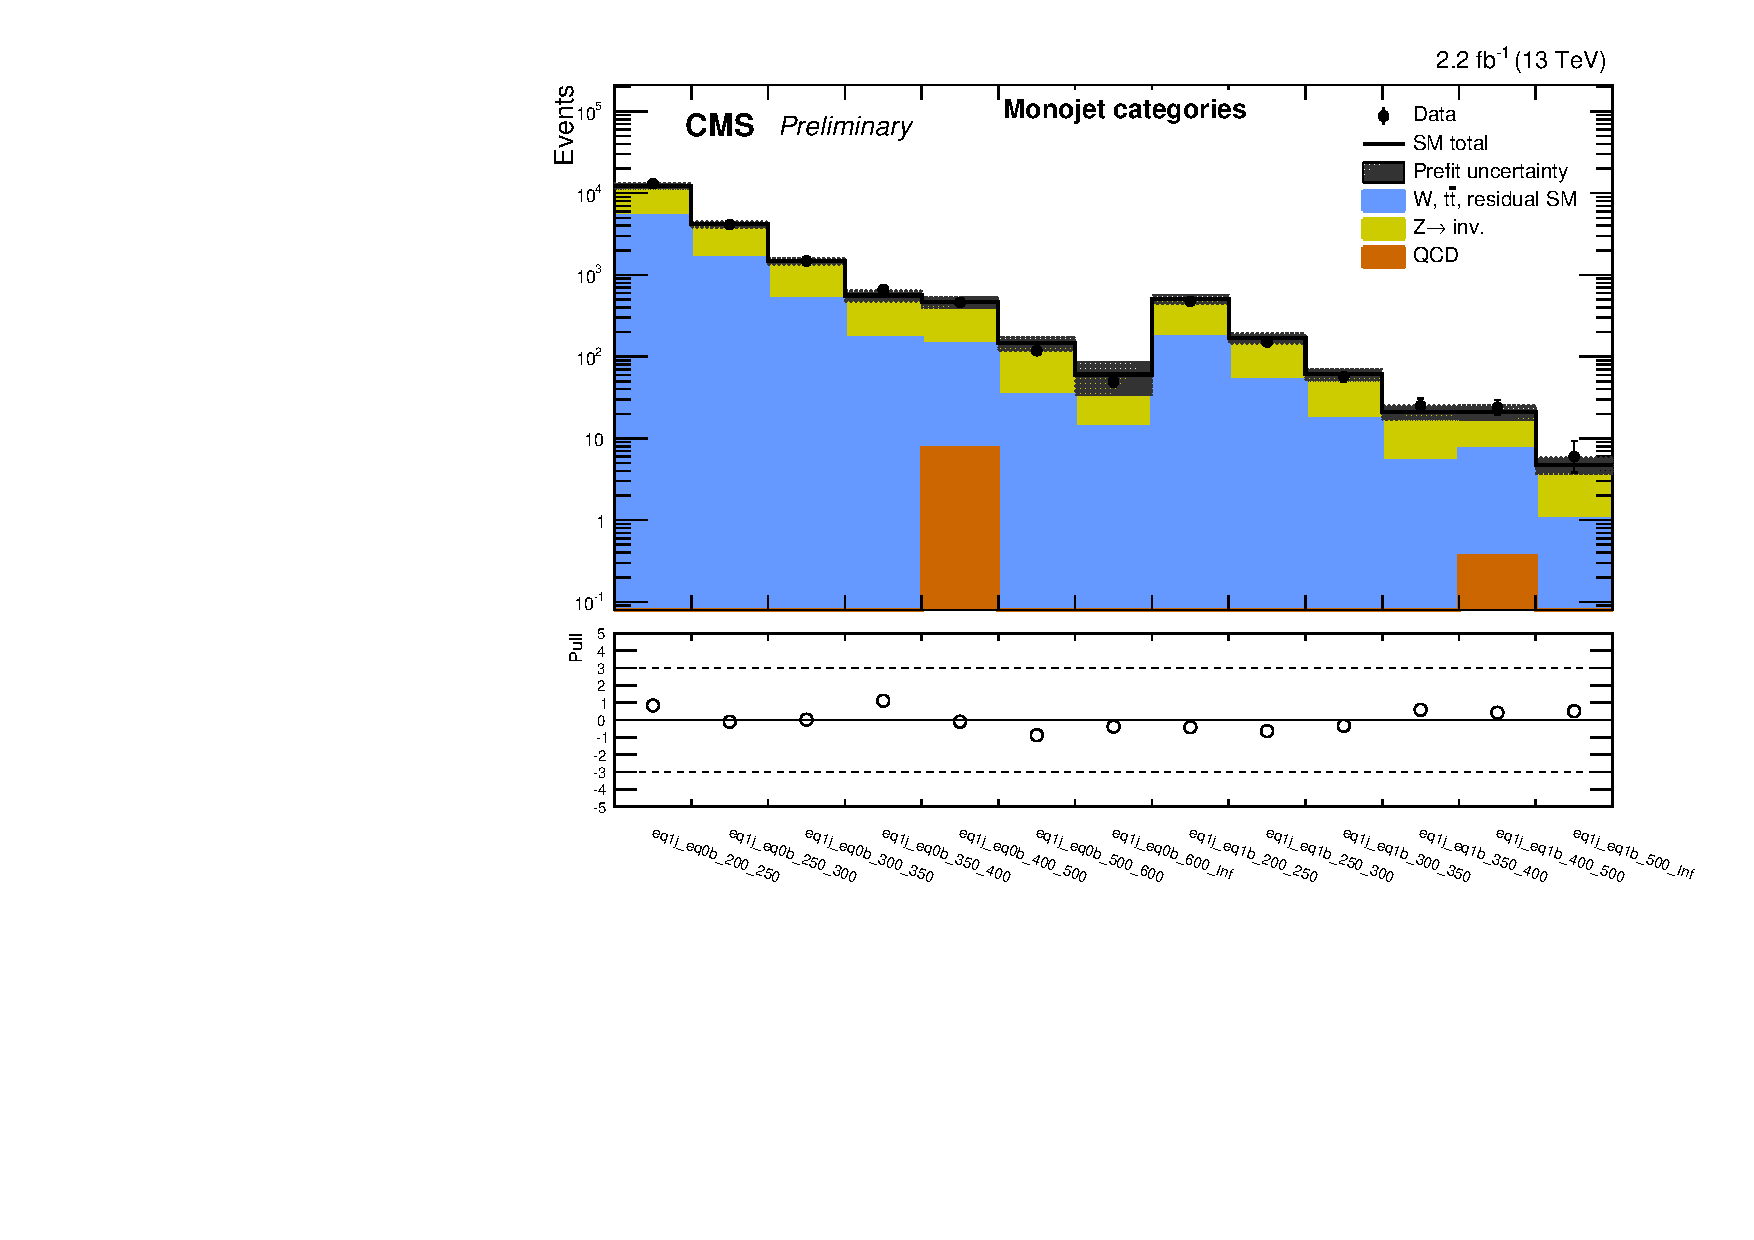
\includegraphics[width=0.8\linewidth]{AN-15-004/trunk/figures/postFitResults/summaryPlots/summaryPlot_prefit_Monojet}
%    \end{figure}
%  \end{center}
%\end{landscape}

%\clearpage
%\begin{landscape}
%  \begin{center}
%    \begin{figure}[h!]
%      \caption{Pre-fit background yields and data obervation for all the (\njet,\nb,\scalht) analysis bins (integrated over \MHT), for the asymmetric topologies. \label{fig:summaryPlot_prefit_Asymmetric}}.
%      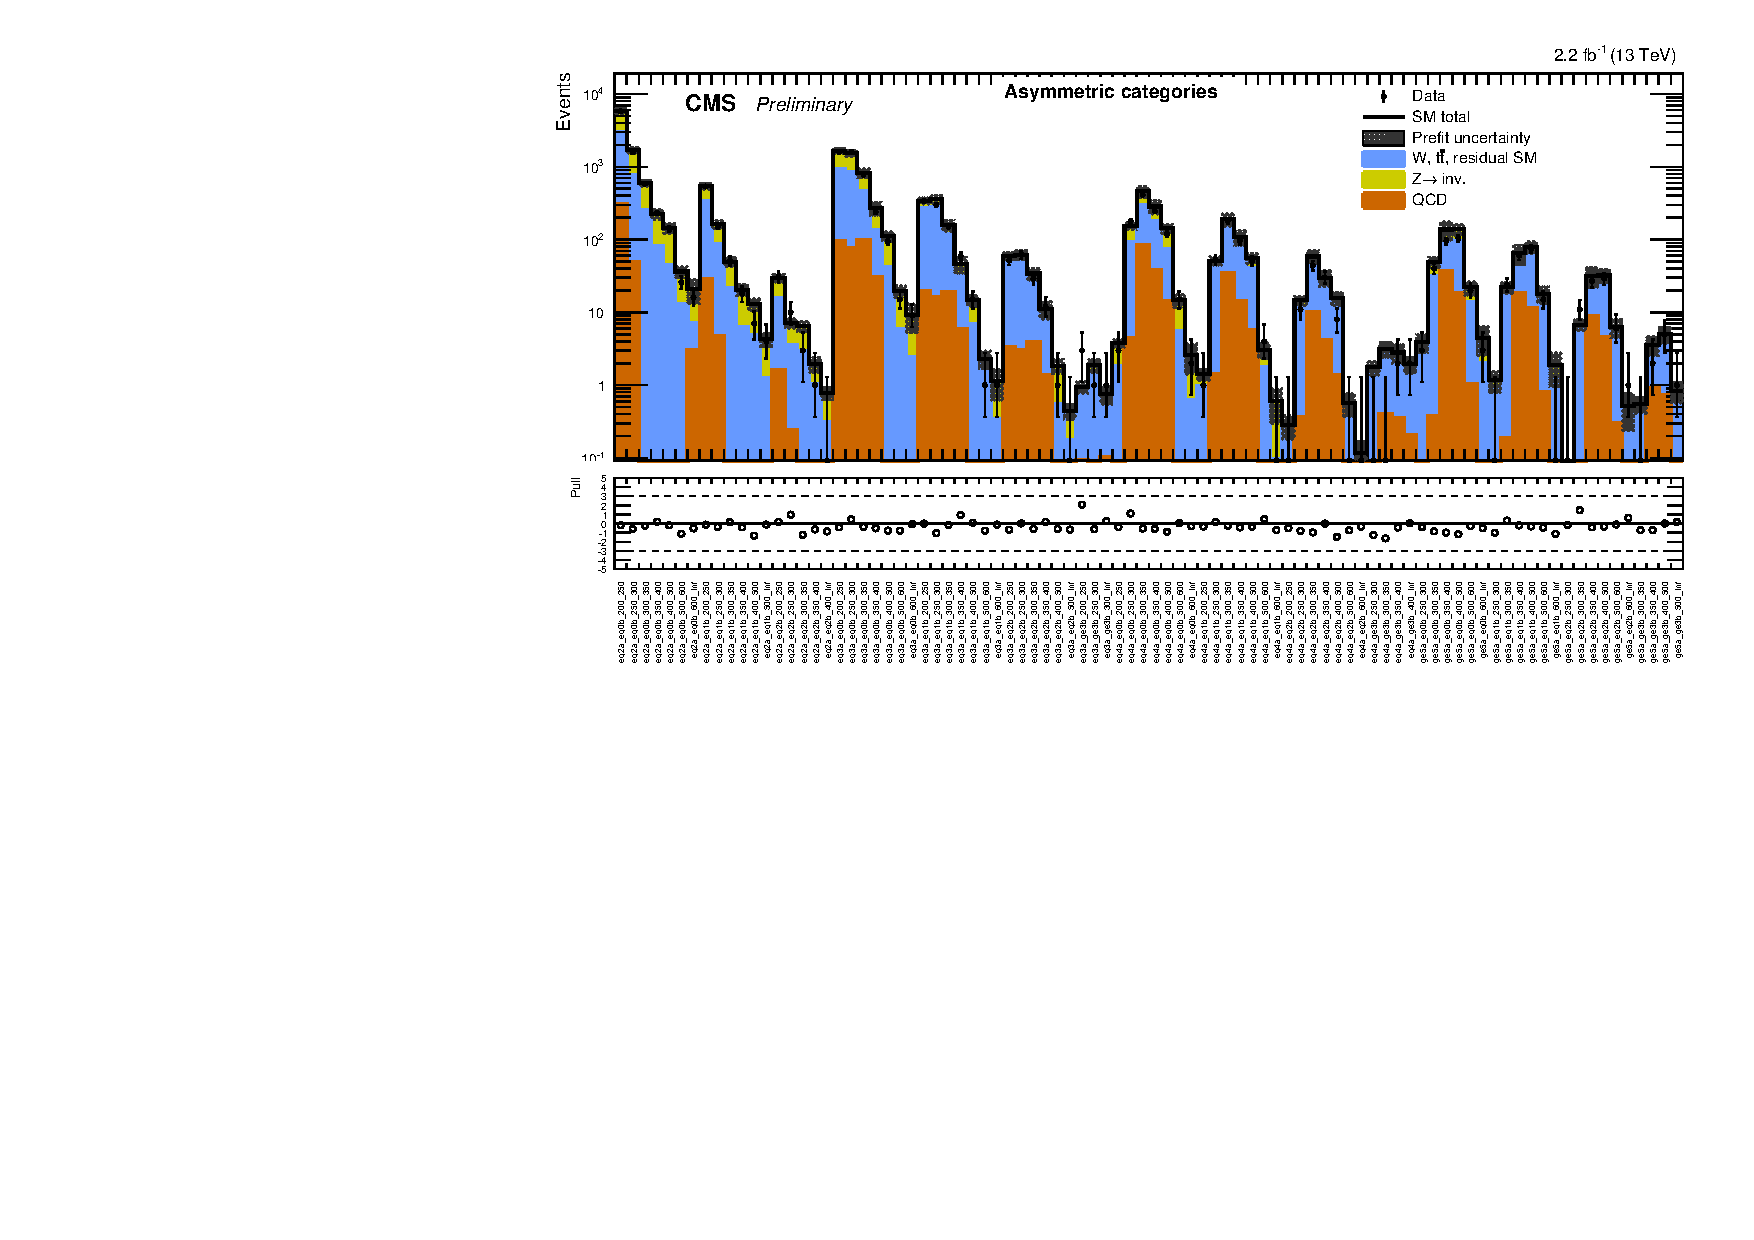
\includegraphics[width=0.8\linewidth]{AN-15-004/trunk/figures/postFitResults/summaryPlots/summaryPlot_prefit_Asymmetric}
%    \end{figure}
%  \end{center}
%\end{landscape}

%\clearpage
%\begin{landscape}
%  \begin{center}
%    \begin{figure}[h!]
%      \caption{Pre-fit background yields and data obervation for all the (\njet,\nb,\scalht) analysis bins (integrated over \MHT), for the symmetric topologies. \label{fig:summaryPlot_prefit_Symmetric}}.
%      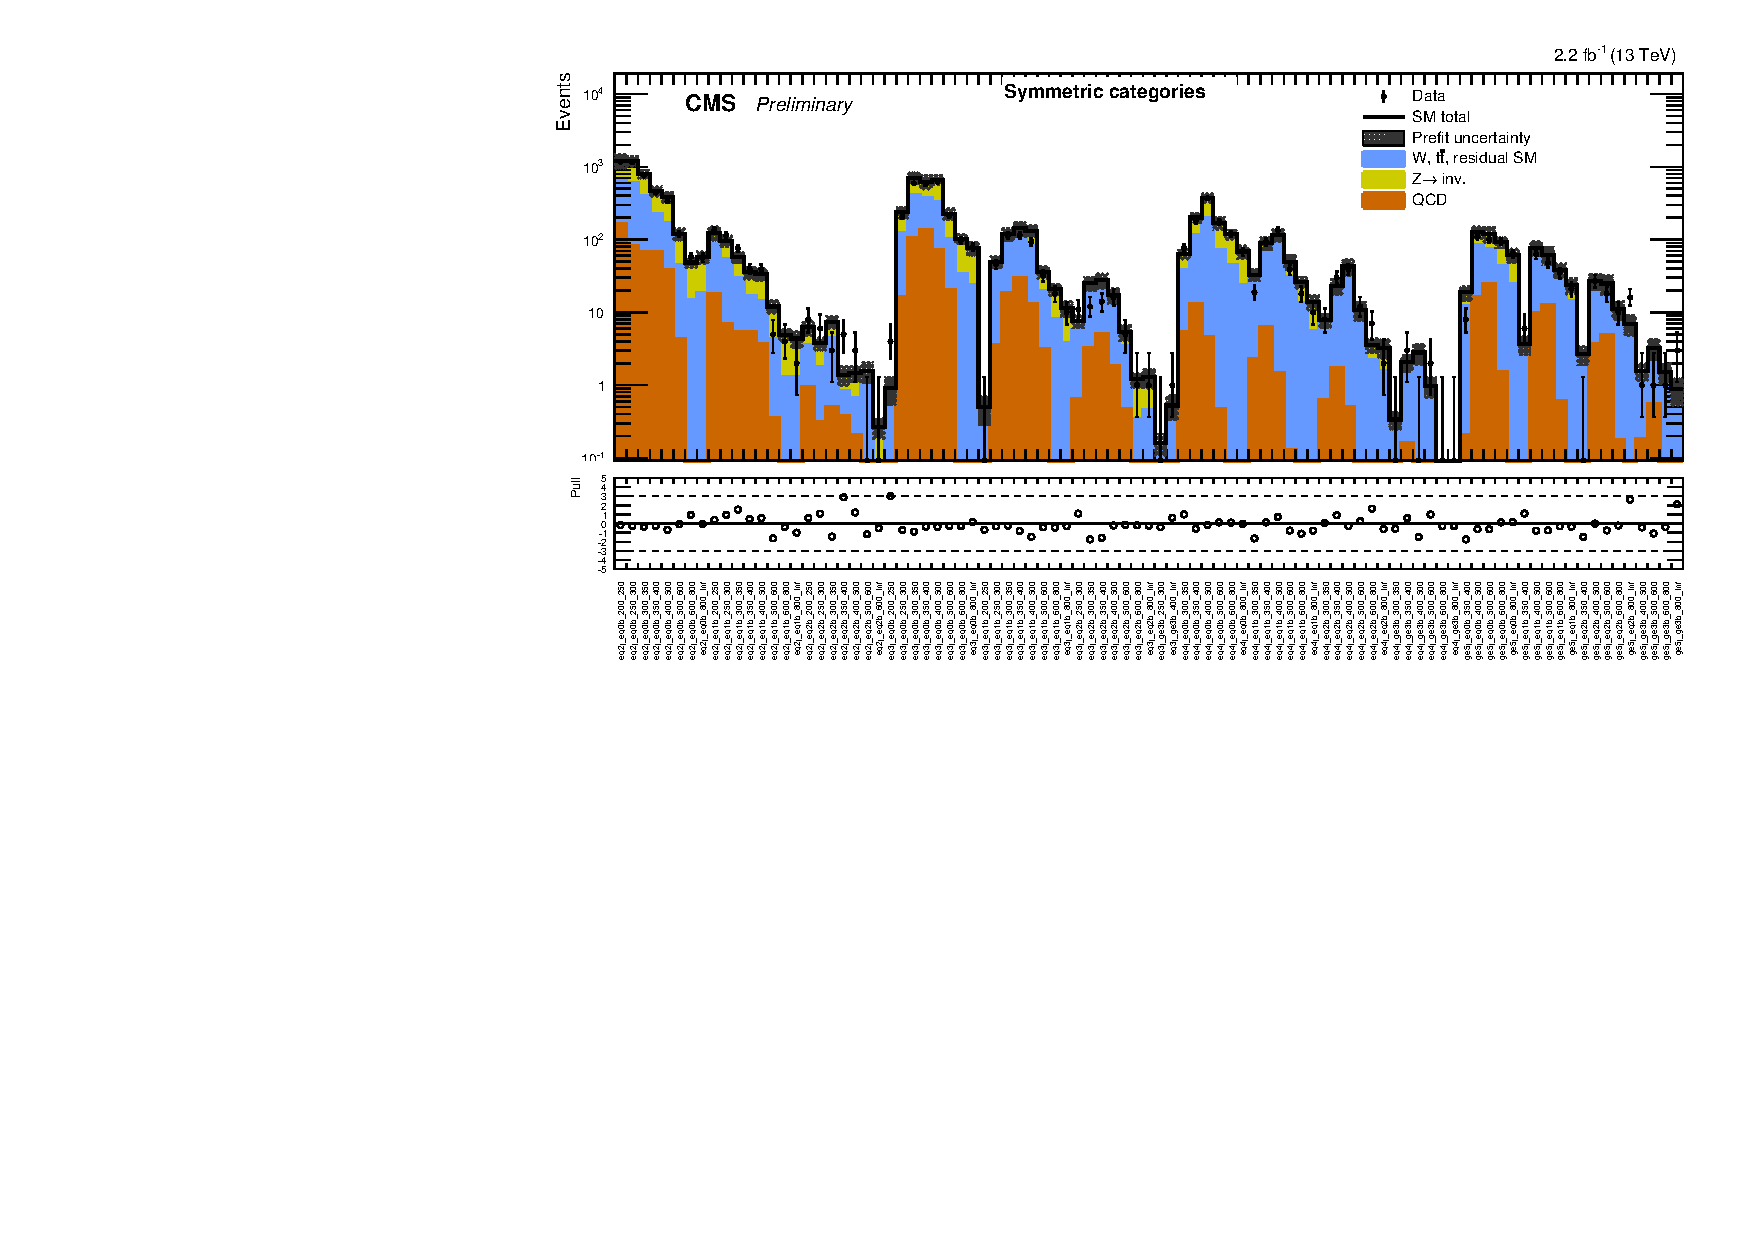
\includegraphics[width=0.8\linewidth]{AN-15-004/trunk/figures/postFitResults/summaryPlots/summaryPlot_prefit_Symmetric}
%    \end{figure}
%  \end{center}
%\end{landscape}


%%%% Post-fit summary plots
\clearpage
\begin{landscape}
  \begin{center}
    \begin{figure}[h!]
      \caption{Post-fit (background-only fit) background yields and data obervation for all the (\njet,\nb,\scalht) analysis bins (integrated over \MHT), for the monojet topologies. \label{fig:summaryPlot_fit_b_Monojet}}.
      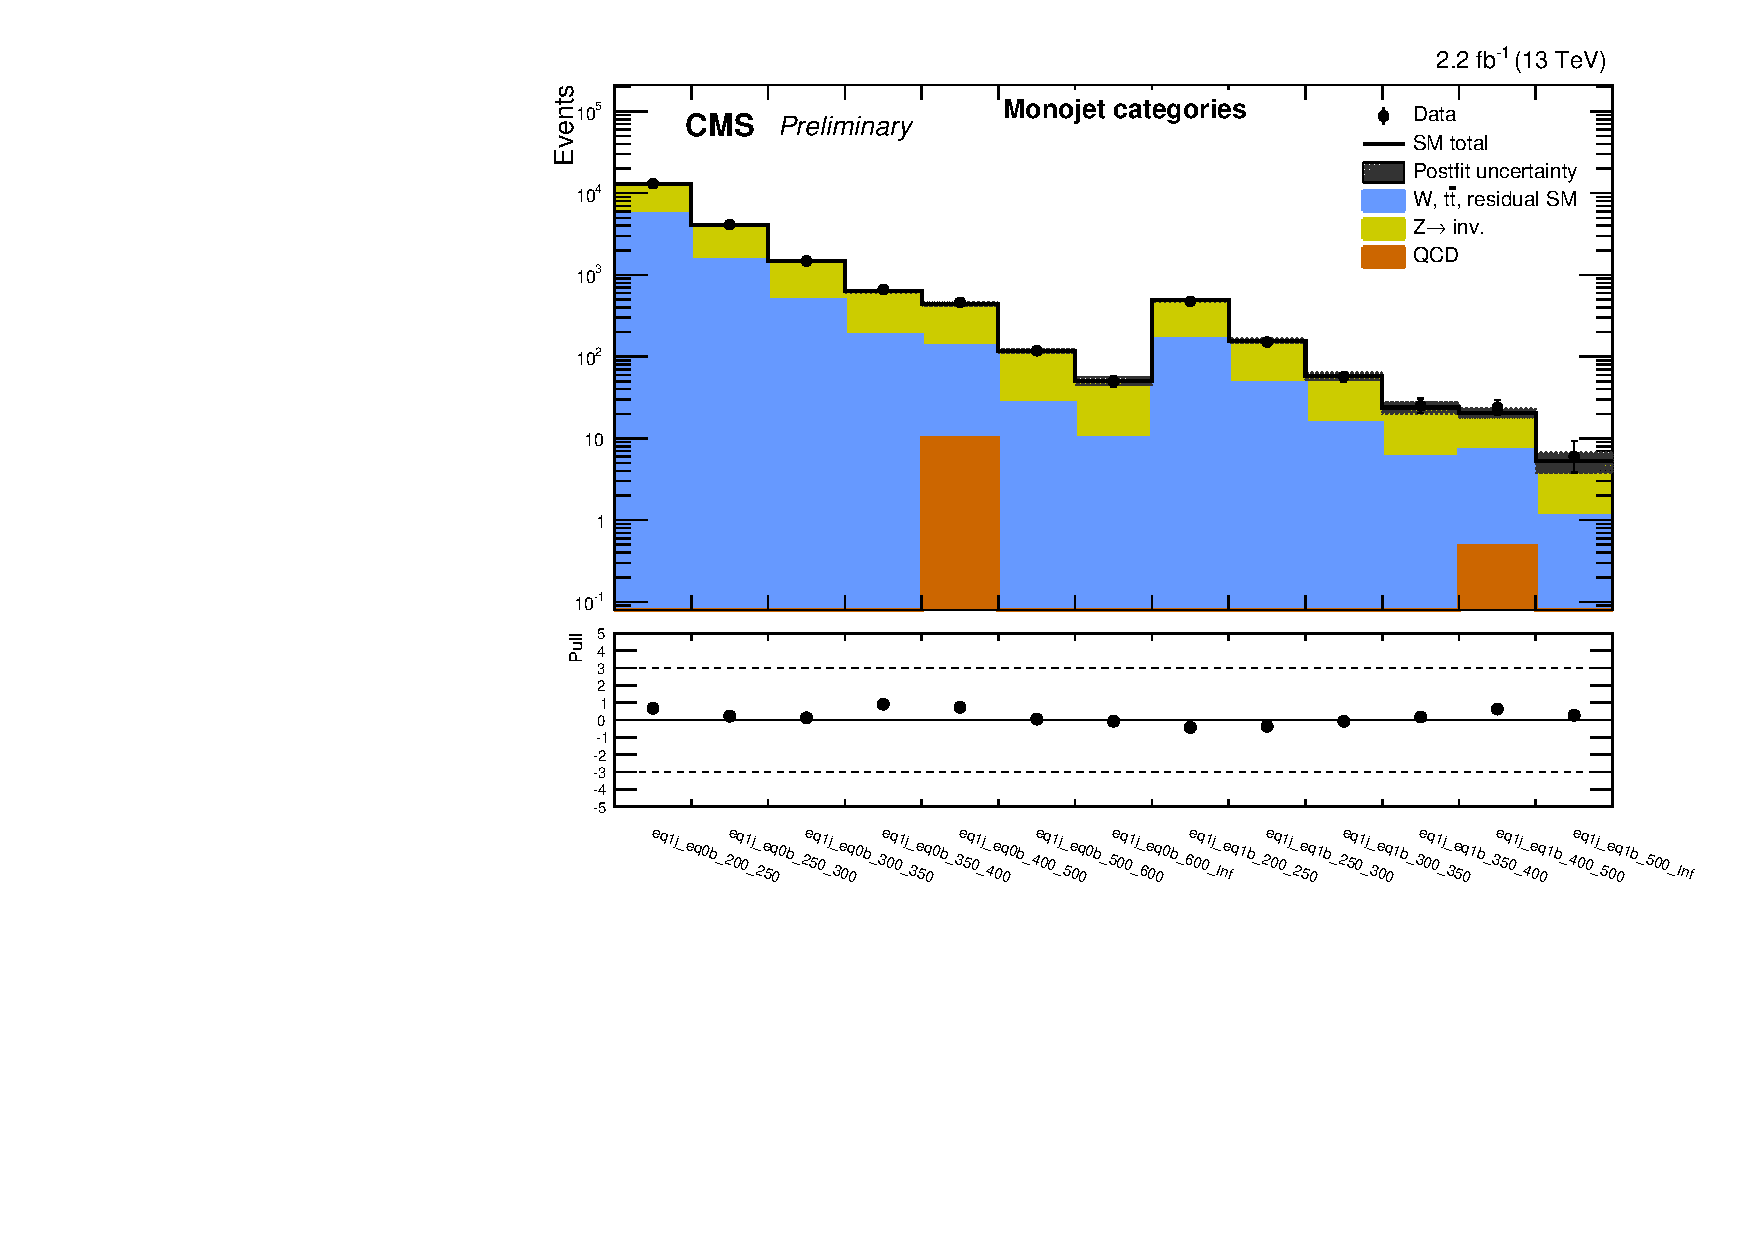
\includegraphics[width=0.8\linewidth]{AN-15-004/trunk/figures/postFitResults/summaryPlots/summaryPlot_fit_b_Monojet}
    \end{figure}
  \end{center}
\end{landscape}

\clearpage
\begin{landscape}
  \begin{center}
    \begin{figure}[h!]
      \caption{Post-fit (background-only fit) background yields and data obervation for all the (\njet,\nb,\scalht) analysis bins (integrated over \MHT), for the asymmetric topologies. \label{fig:summaryPlot_fit_b_Asymmetric}}.
      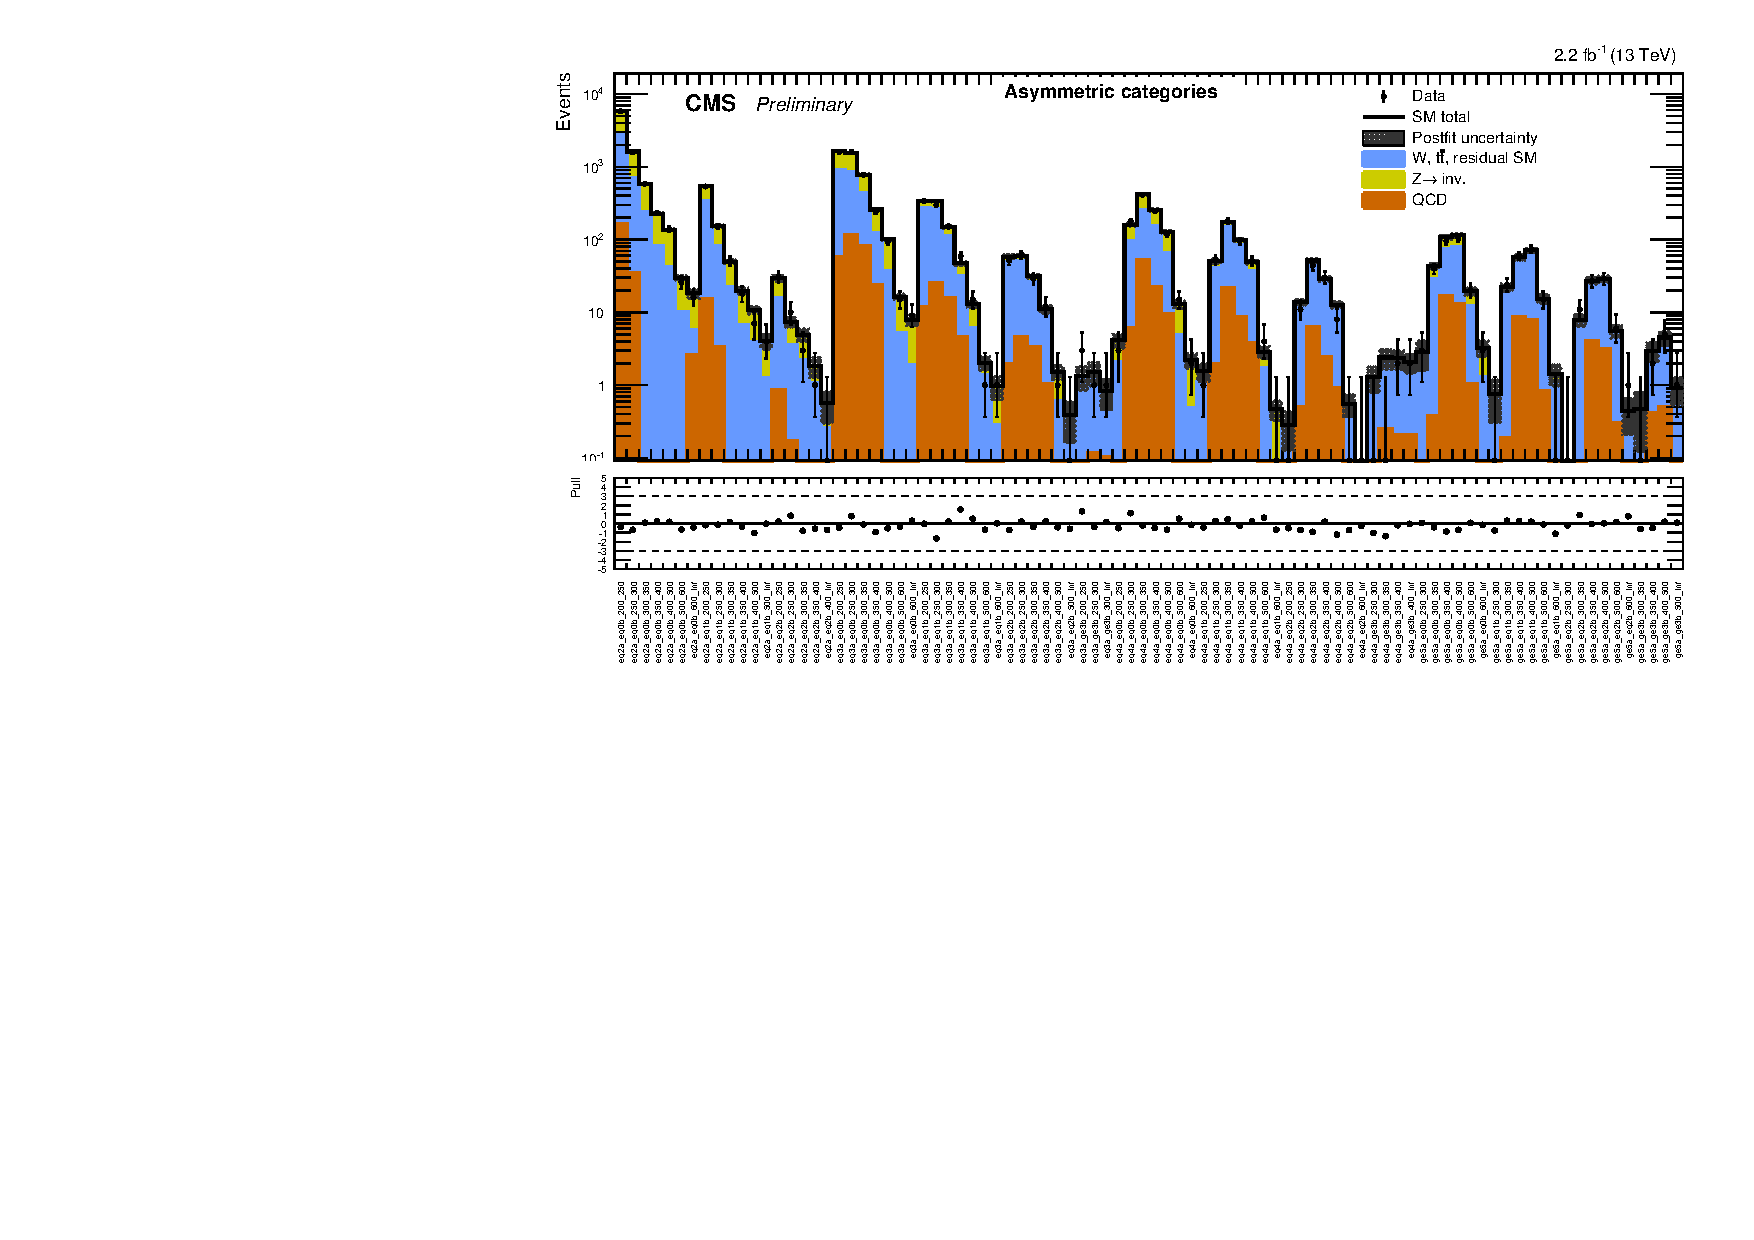
\includegraphics[width=0.8\linewidth]{AN-15-004/trunk/figures/postFitResults/summaryPlots/summaryPlot_fit_b_Asymmetric}
    \end{figure}
  \end{center}
\end{landscape}

\clearpage
\begin{landscape}
  \begin{center}
    \begin{figure}[h!]
      \caption{Post-fit (background-only fit) background yields and data obervation for all the (\njet,\nb,\scalht) analysis bins (integrated over \MHT), for the symmetric topologies. \label{fig:summaryPlot_fit_b_Symmetric}}.
      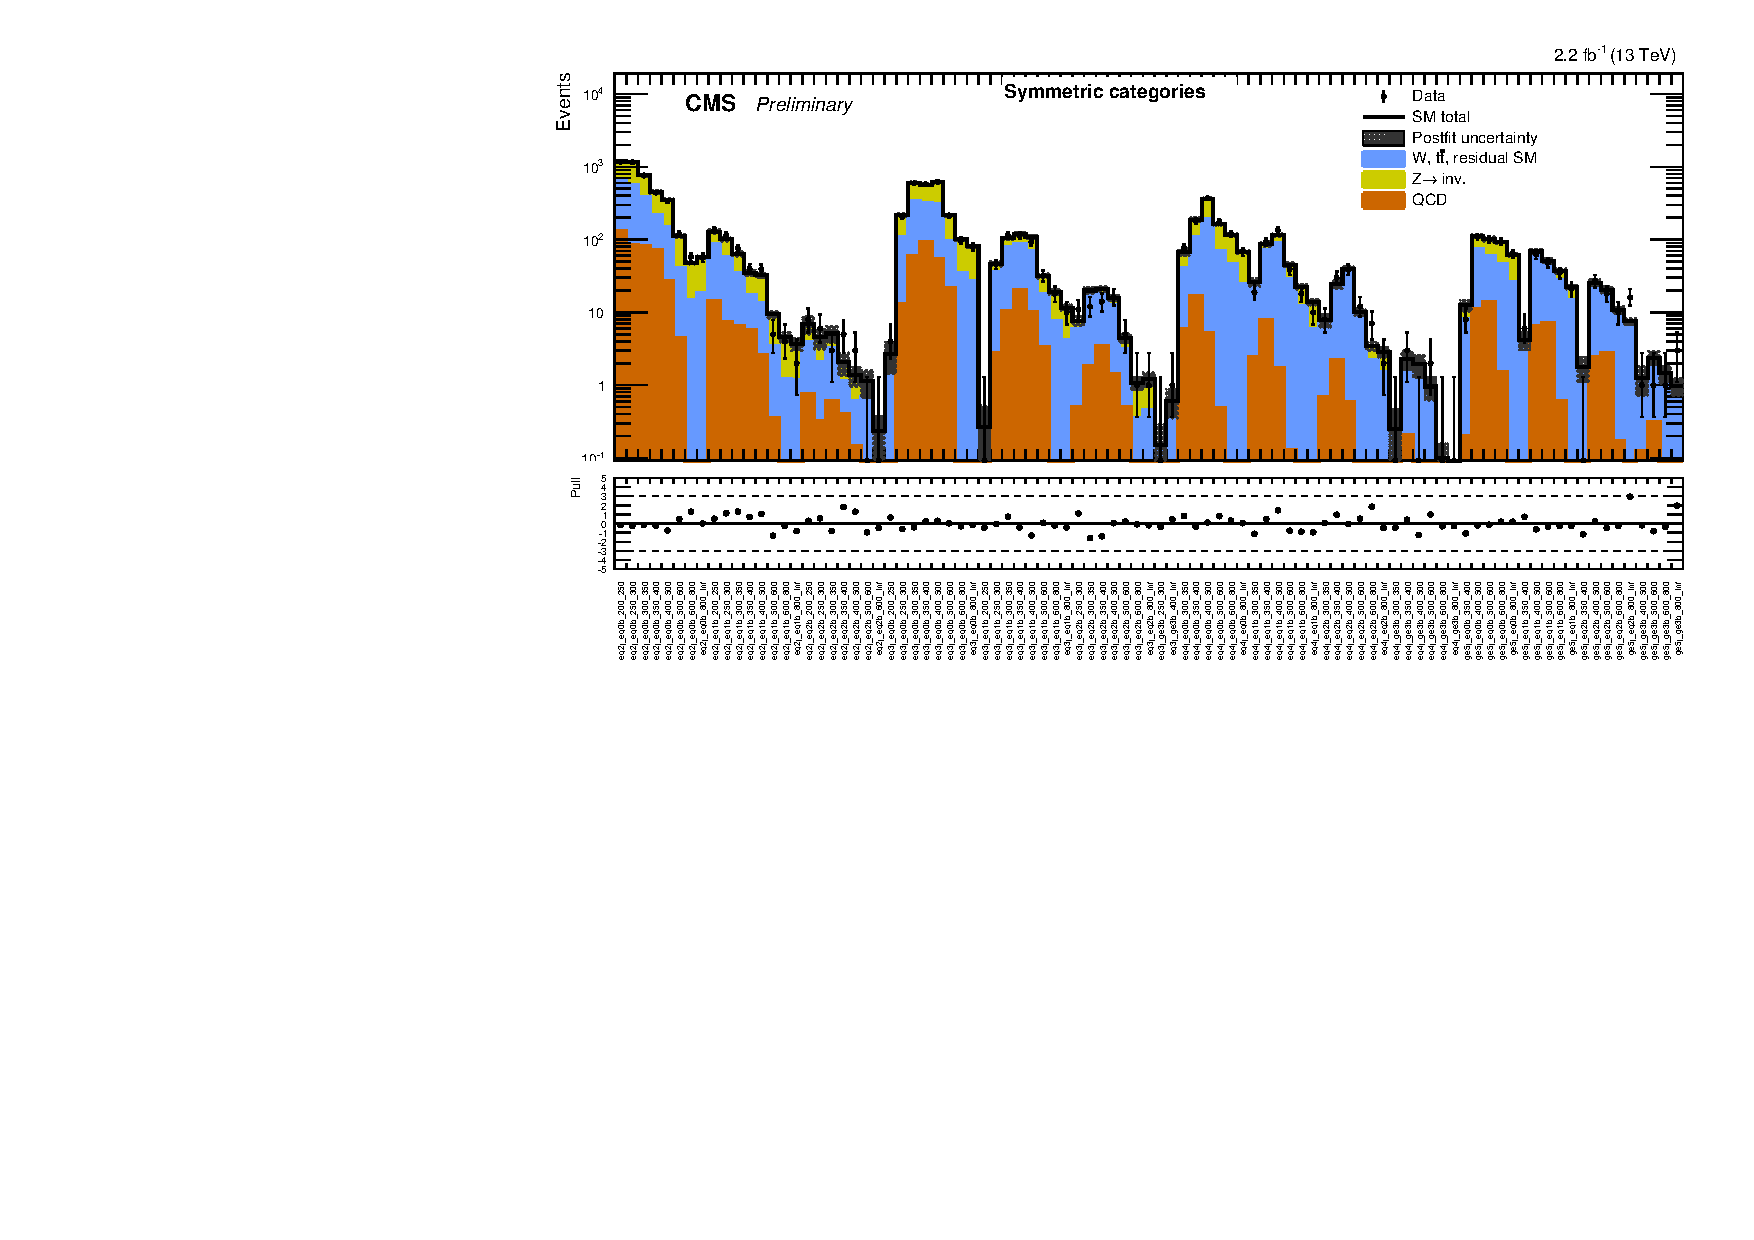
\includegraphics[width=0.8\linewidth]{AN-15-004/trunk/figures/postFitResults/summaryPlots/summaryPlot_fit_b_Symmetric}
    \end{figure}
  \end{center}
\end{landscape}




%\clearpage
%\begin{figure}[tbhp]
%    \caption{ Pull of the nuisances parameters associated to the \alt-extrapolation systematic uncertainty, 
%      for the asymmetric (symmetric) categories on the left (right).
%      \label{fig:nuisPull_AlphaT}}
%  \begin{center}
%    \subfigure[Asymmetric categories]{ 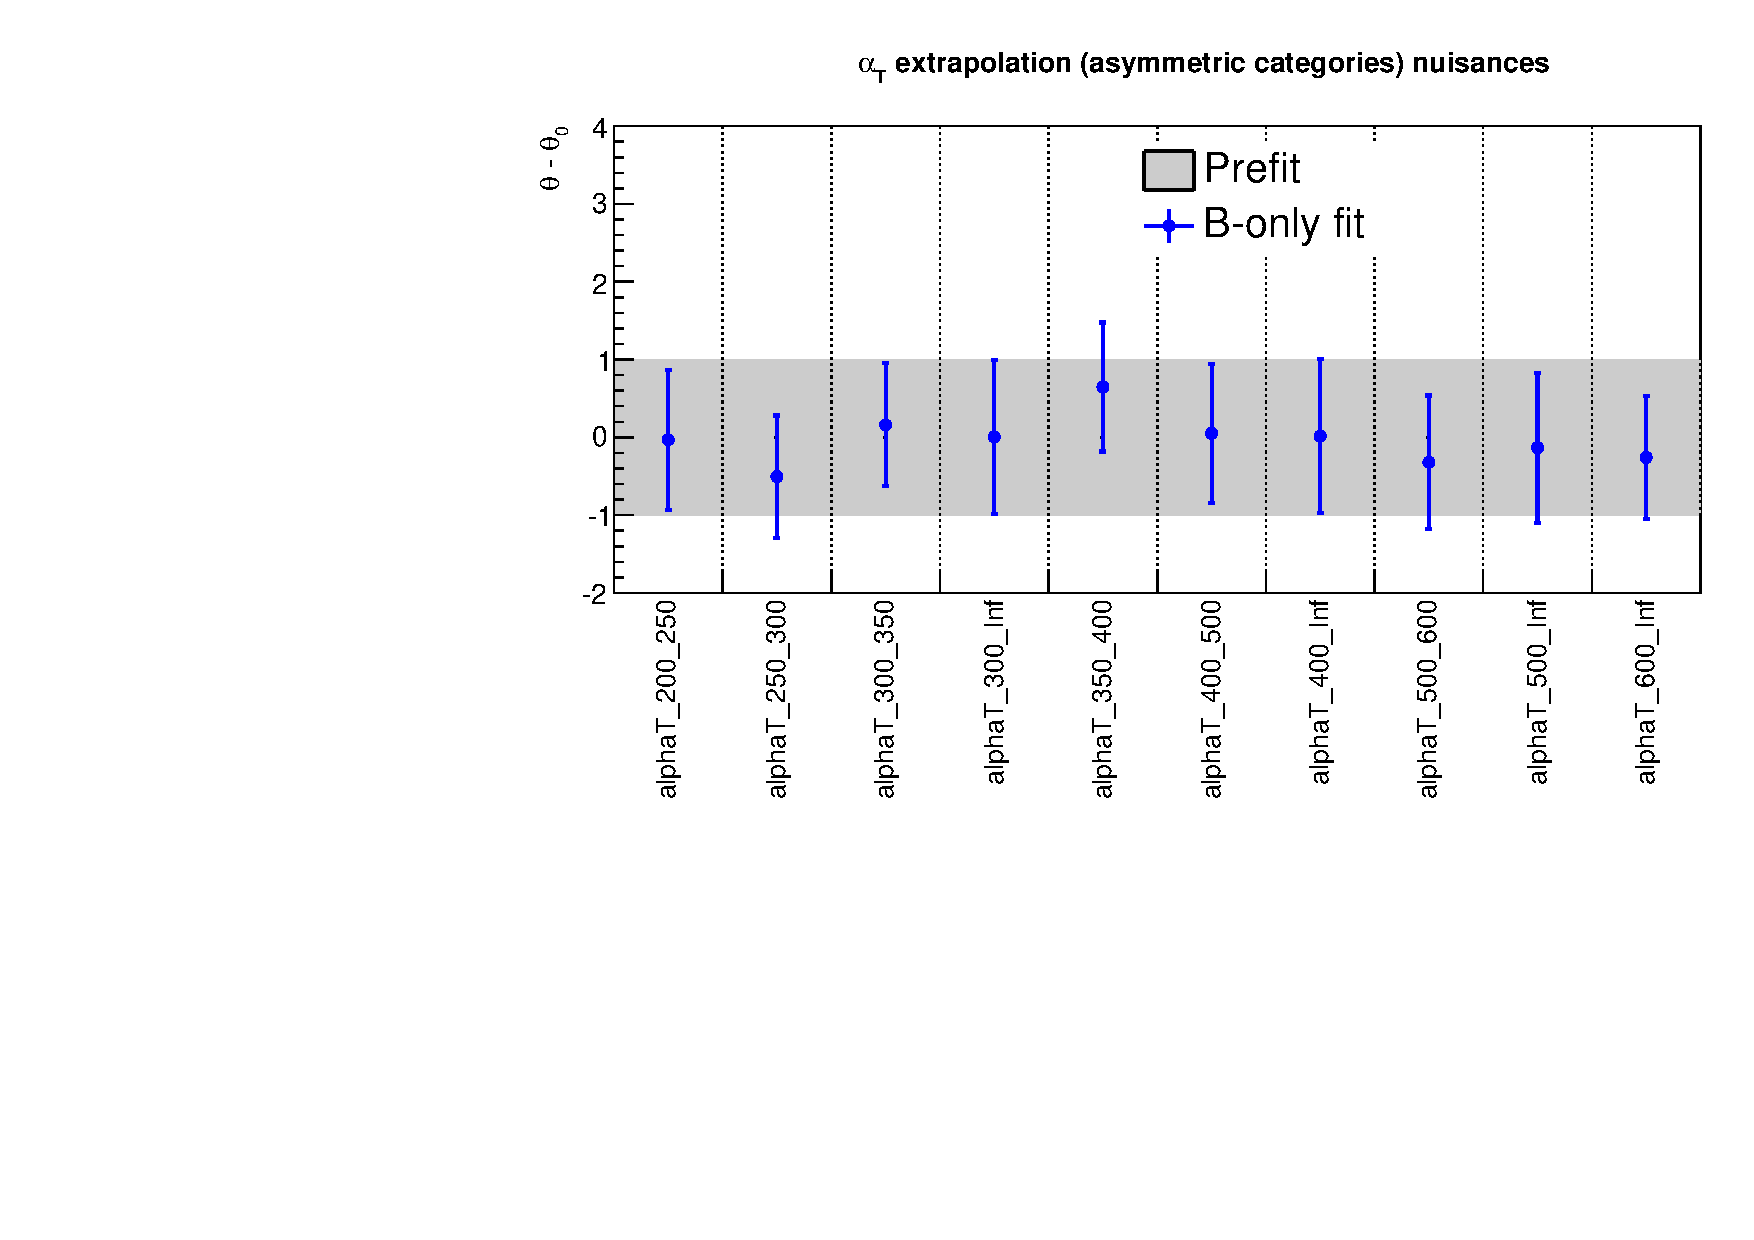
\includegraphics[width=0.45\textwidth]{AN-15-004/trunk/figures/postFitResults/nuisancePlots/AlphaT_asym_nuisances} } ~~
%    \subfigure[Symmetric categories]{ 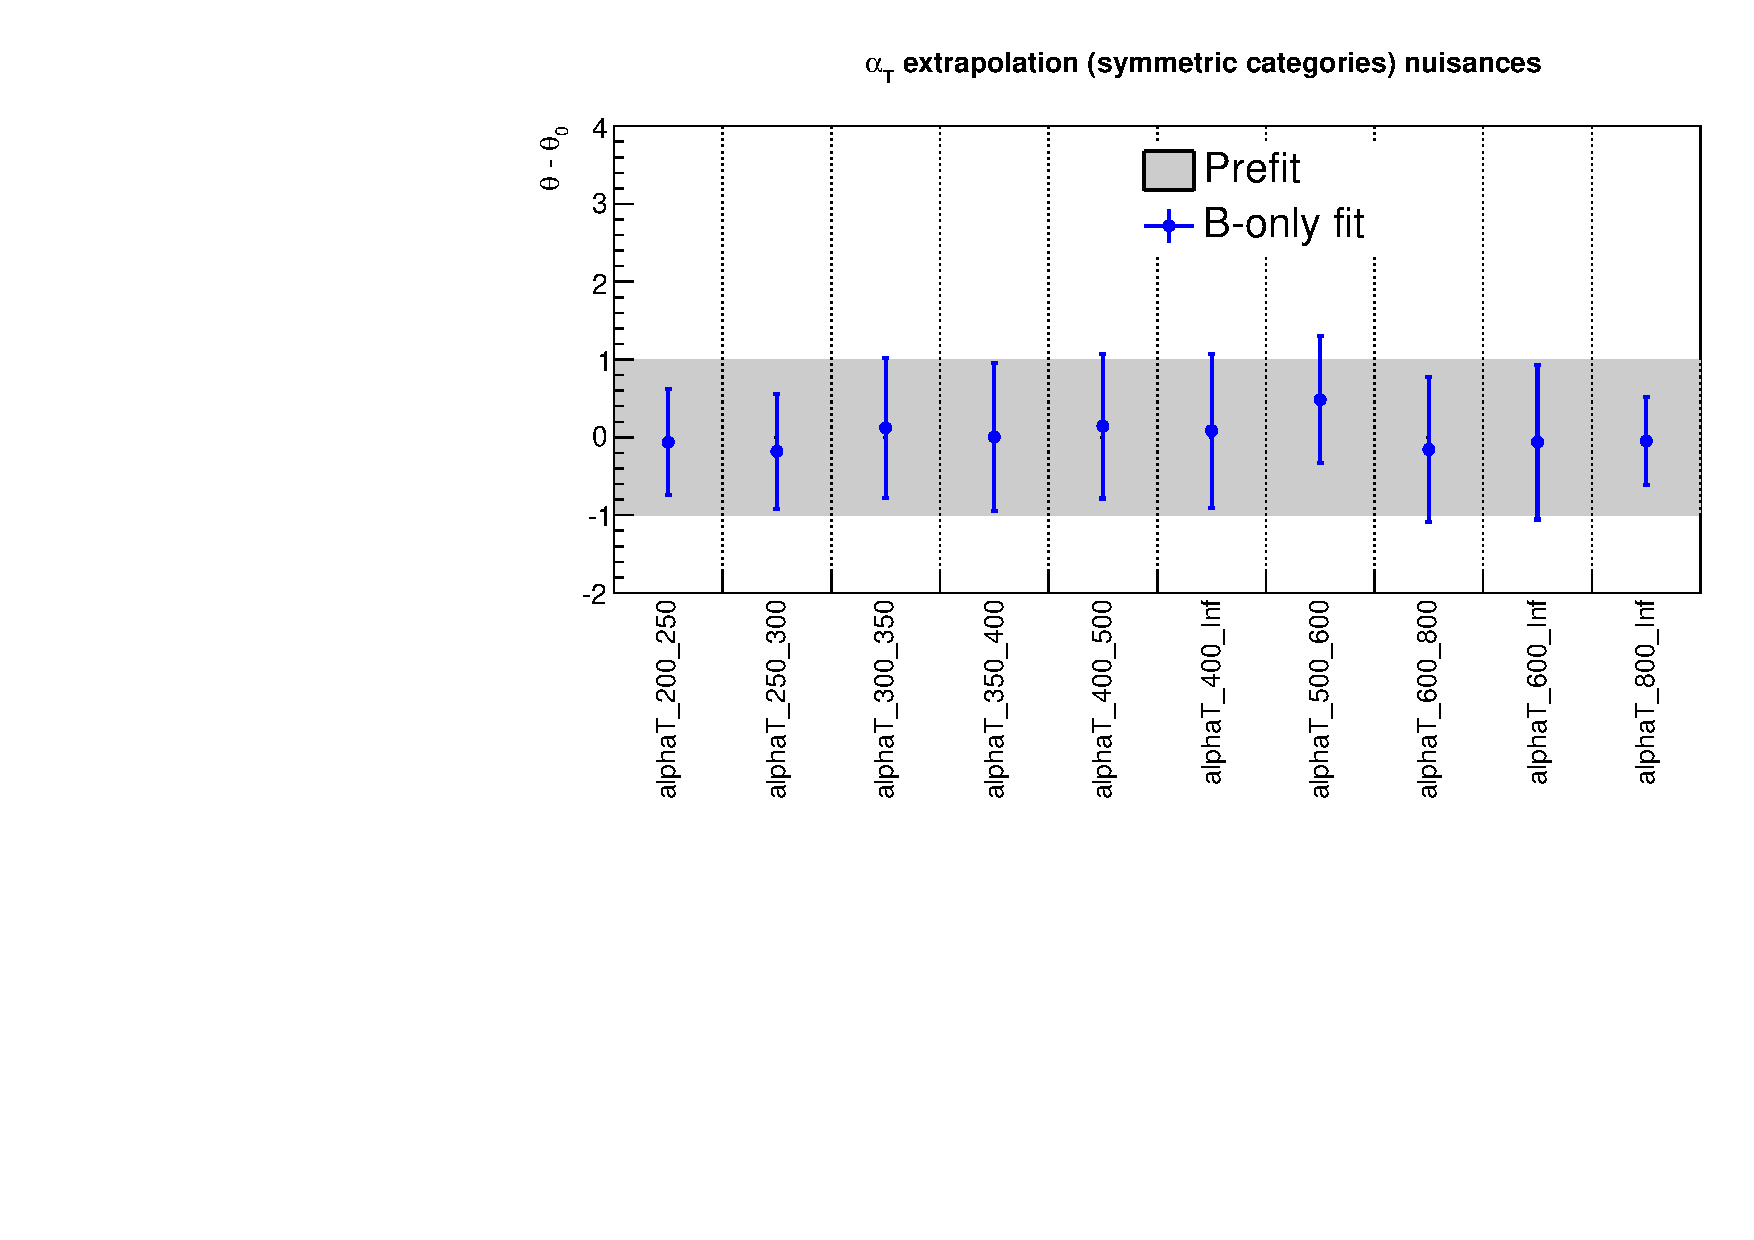
\includegraphics[width=0.45\textwidth]{AN-15-004/trunk/figures/postFitResults/nuisancePlots/AlphaT_sym_nuisances} }
%  \end{center}
%\end{figure}

%\begin{figure}[tbhp]
%    \caption{ Pull of the nuisances parameters associated to the $\gamma/Z$ ratio systematic uncertainty, 
%      for the asymmetric (symmetric) categories on the left (right).
%      \label{fig:nuisPull_gamma_Z_ratio}}
%  \begin{center}
%    \subfigure[Asymmetric categories]{ 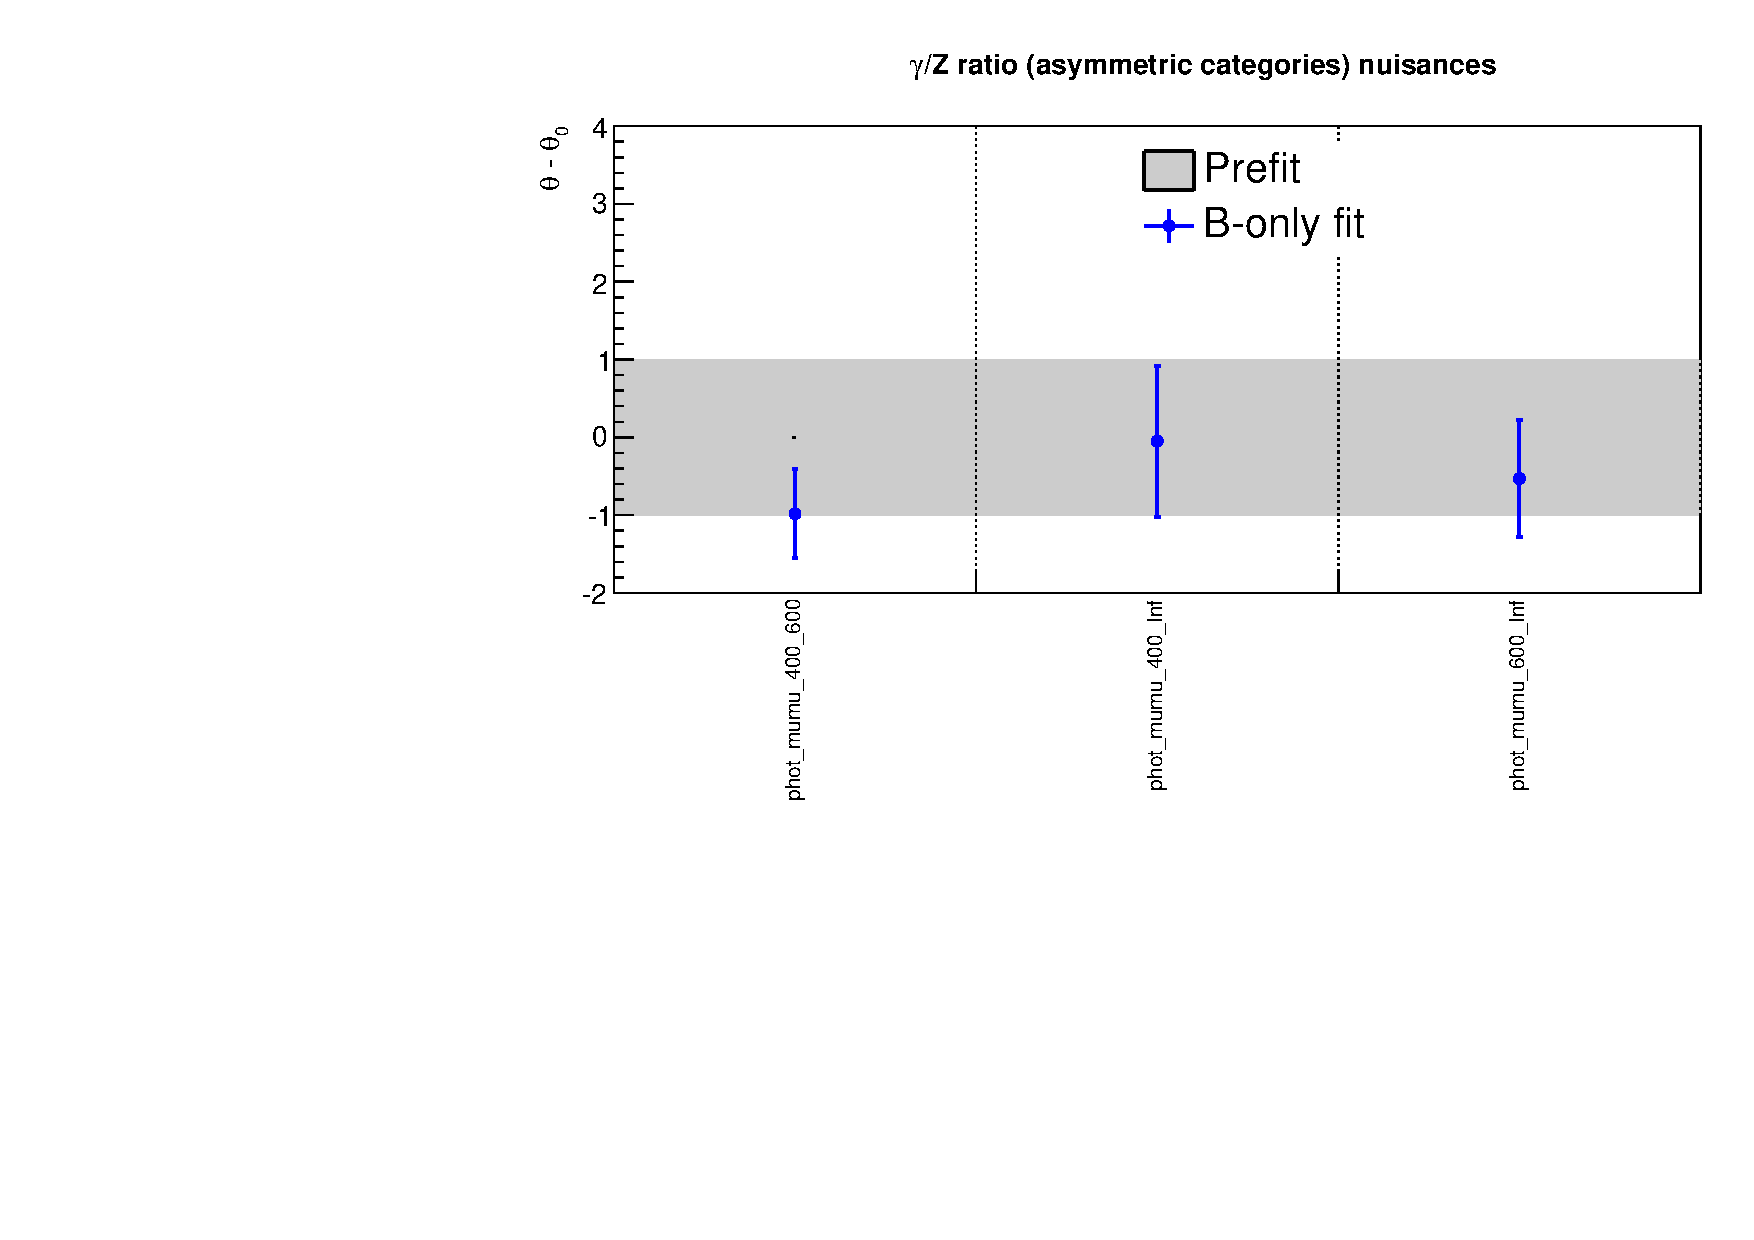
\includegraphics[width=0.45\textwidth]{AN-15-004/trunk/figures/postFitResults/nuisancePlots/gamma_Z_ratio_asym_nuisances} } ~~
%    \subfigure[Symmetric categories]{ 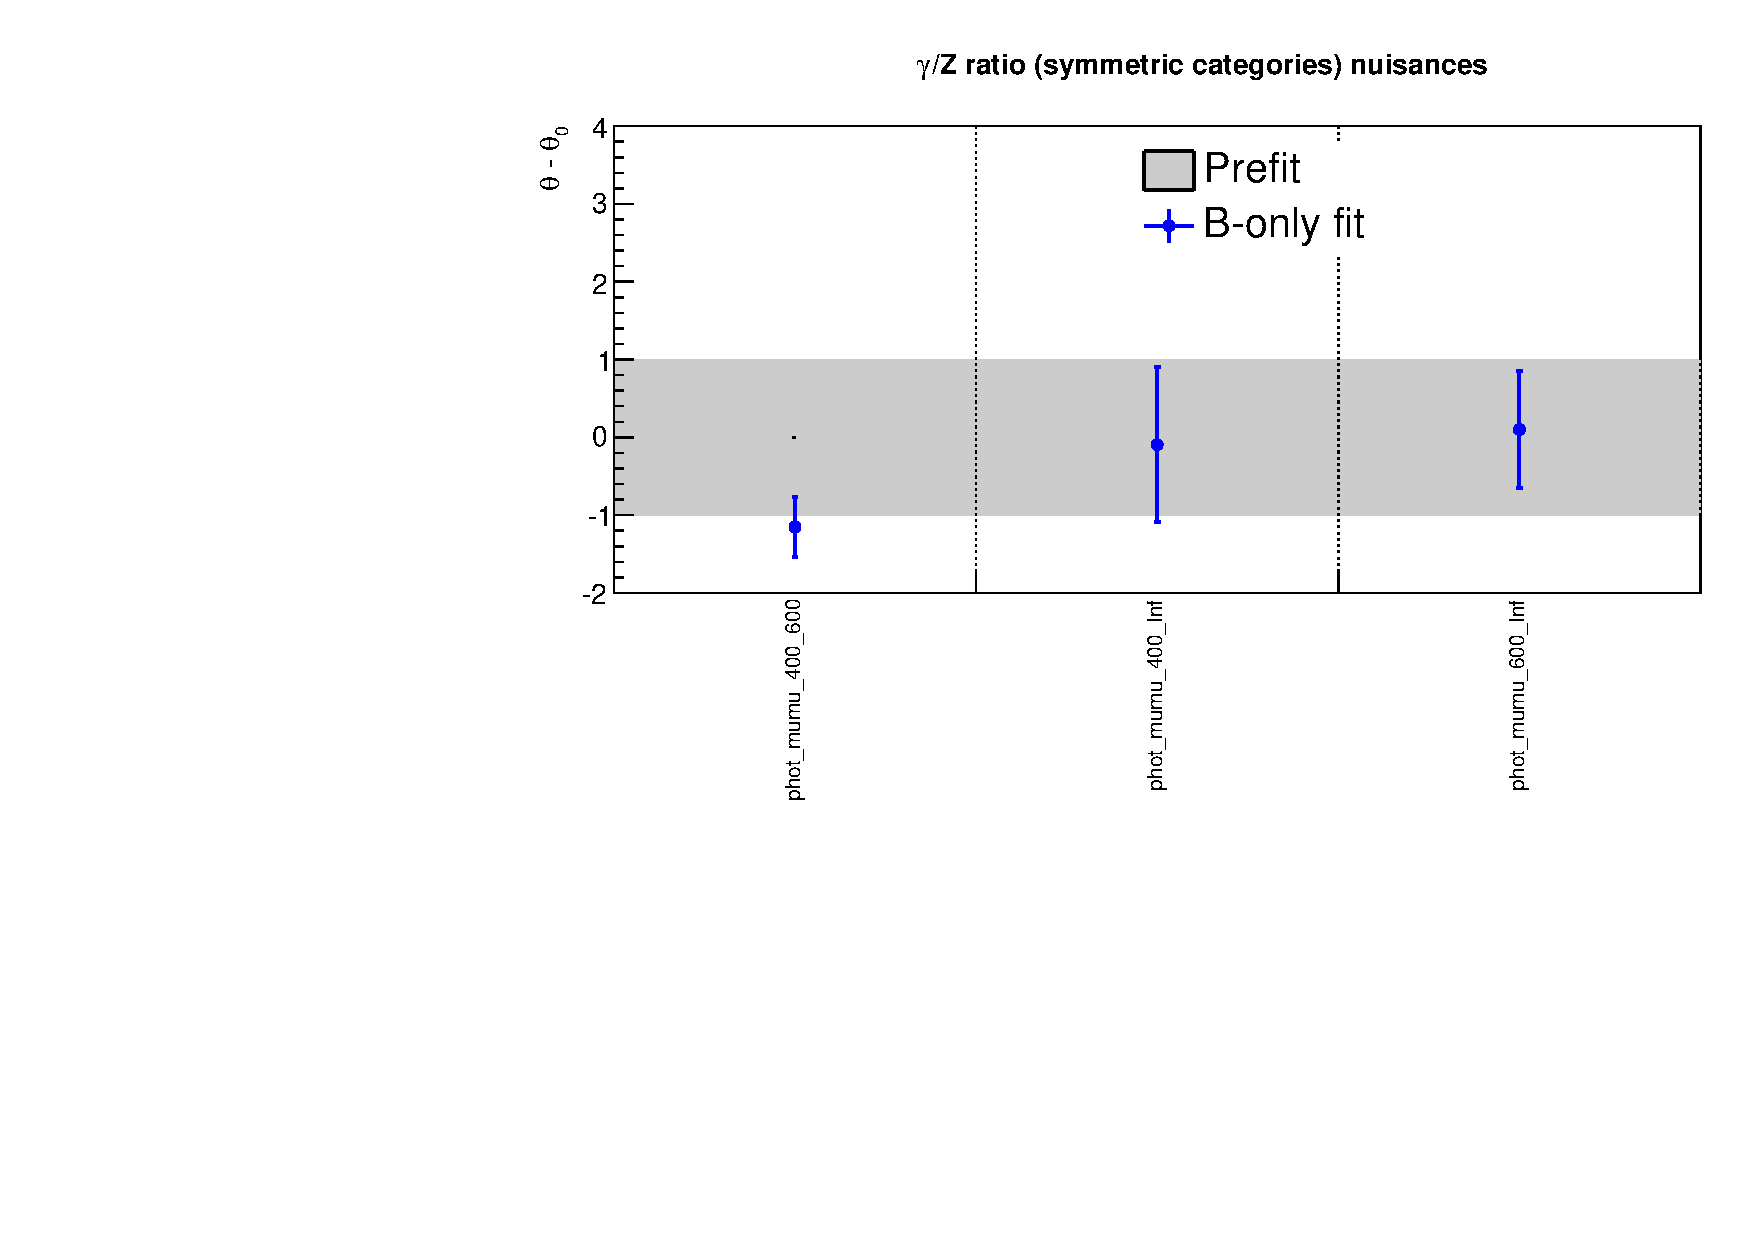
\includegraphics[width=0.45\textwidth]{AN-15-004/trunk/figures/postFitResults/nuisancePlots/gamma_Z_ratio_sym_nuisances} }
%  \end{center}
%\end{figure}

%\begin{figure}[tbhp]
%    \caption{ Pull of the nuisances parameters associated to the $W/Z$ ratio systematic uncertainty, 
%      for the asymmetric (symmetric) categories on the left (right).
%      \label{fig:nuisPull_W_Z_ratio}}
%  \begin{center}
%    \subfigure[Asymmetric categories]{ 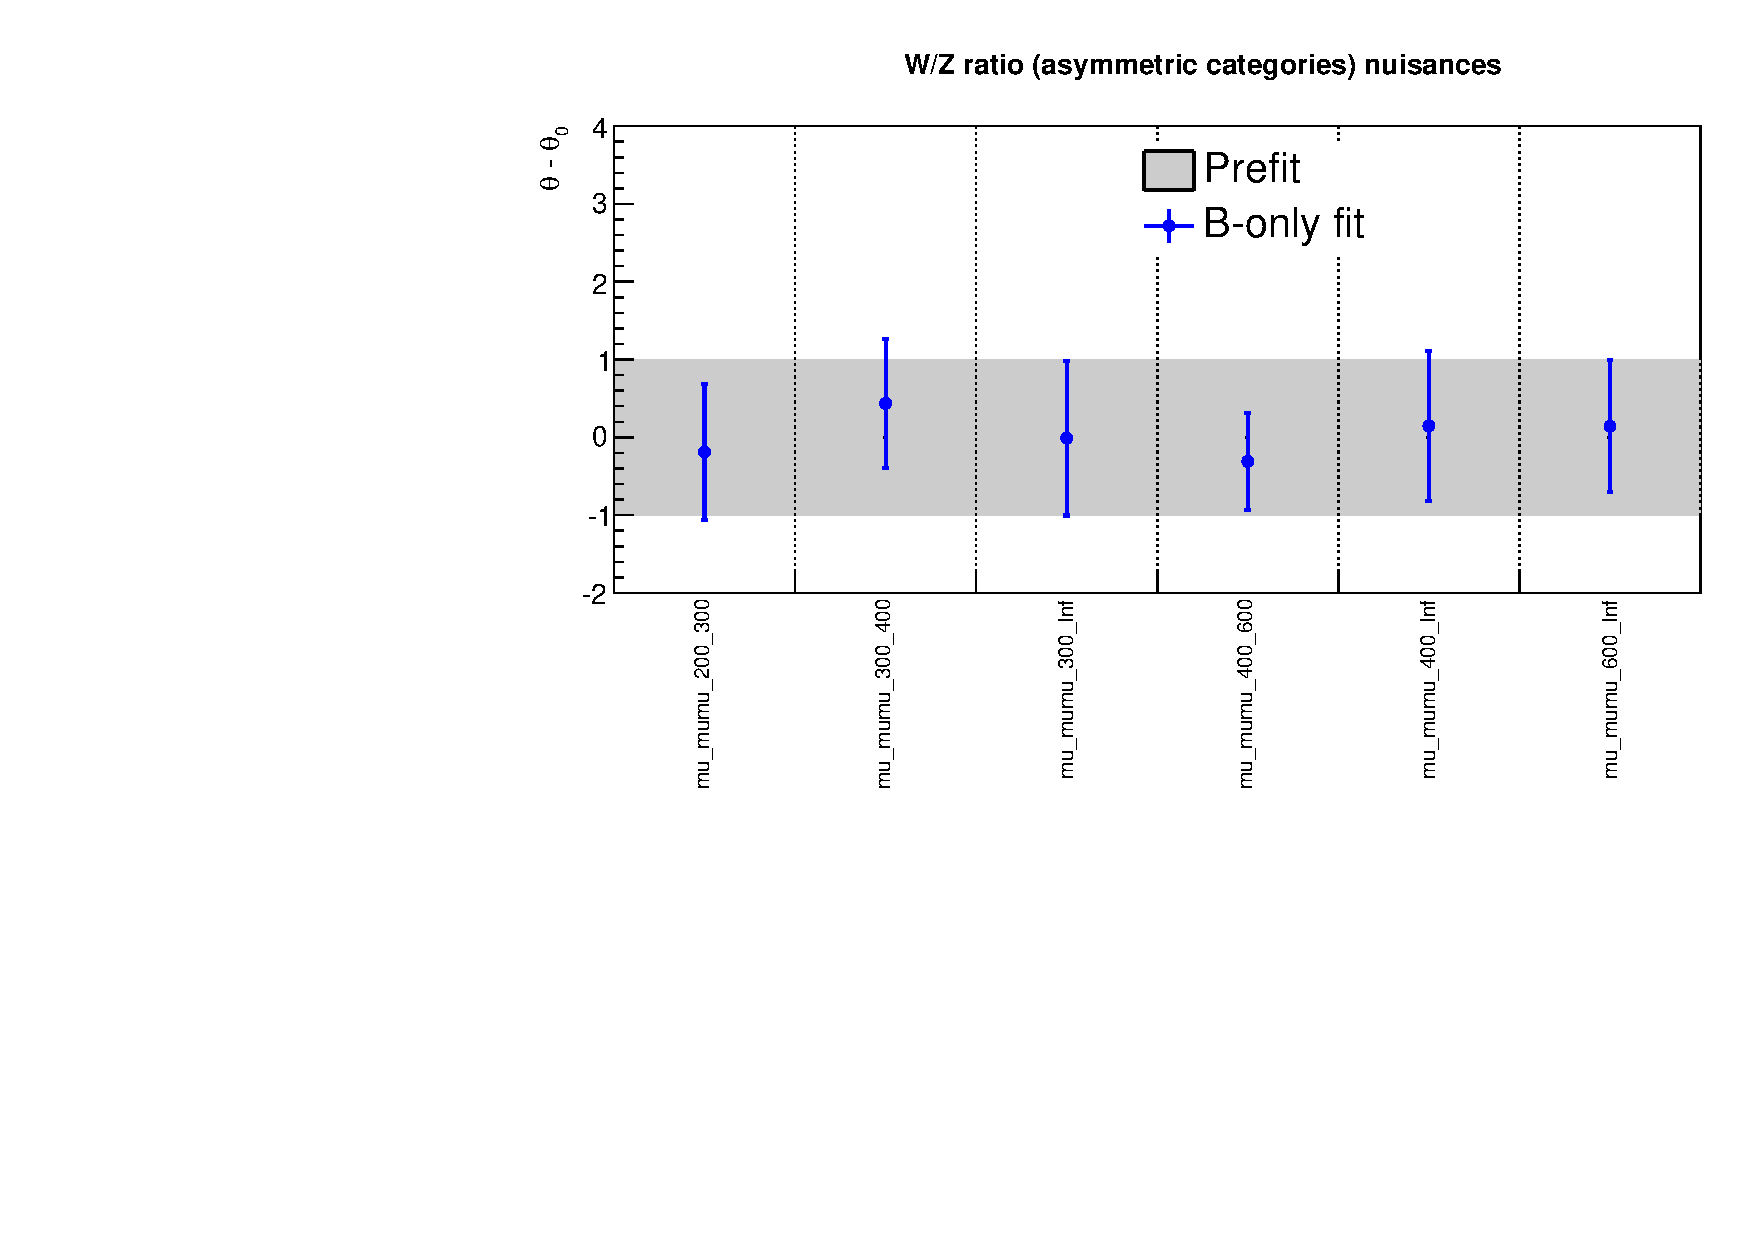
\includegraphics[width=0.45\textwidth]{AN-15-004/trunk/figures/postFitResults/nuisancePlots/W_Z_ratio_asym_nuisances} } ~~
%    \subfigure[Symmetric categories]{ 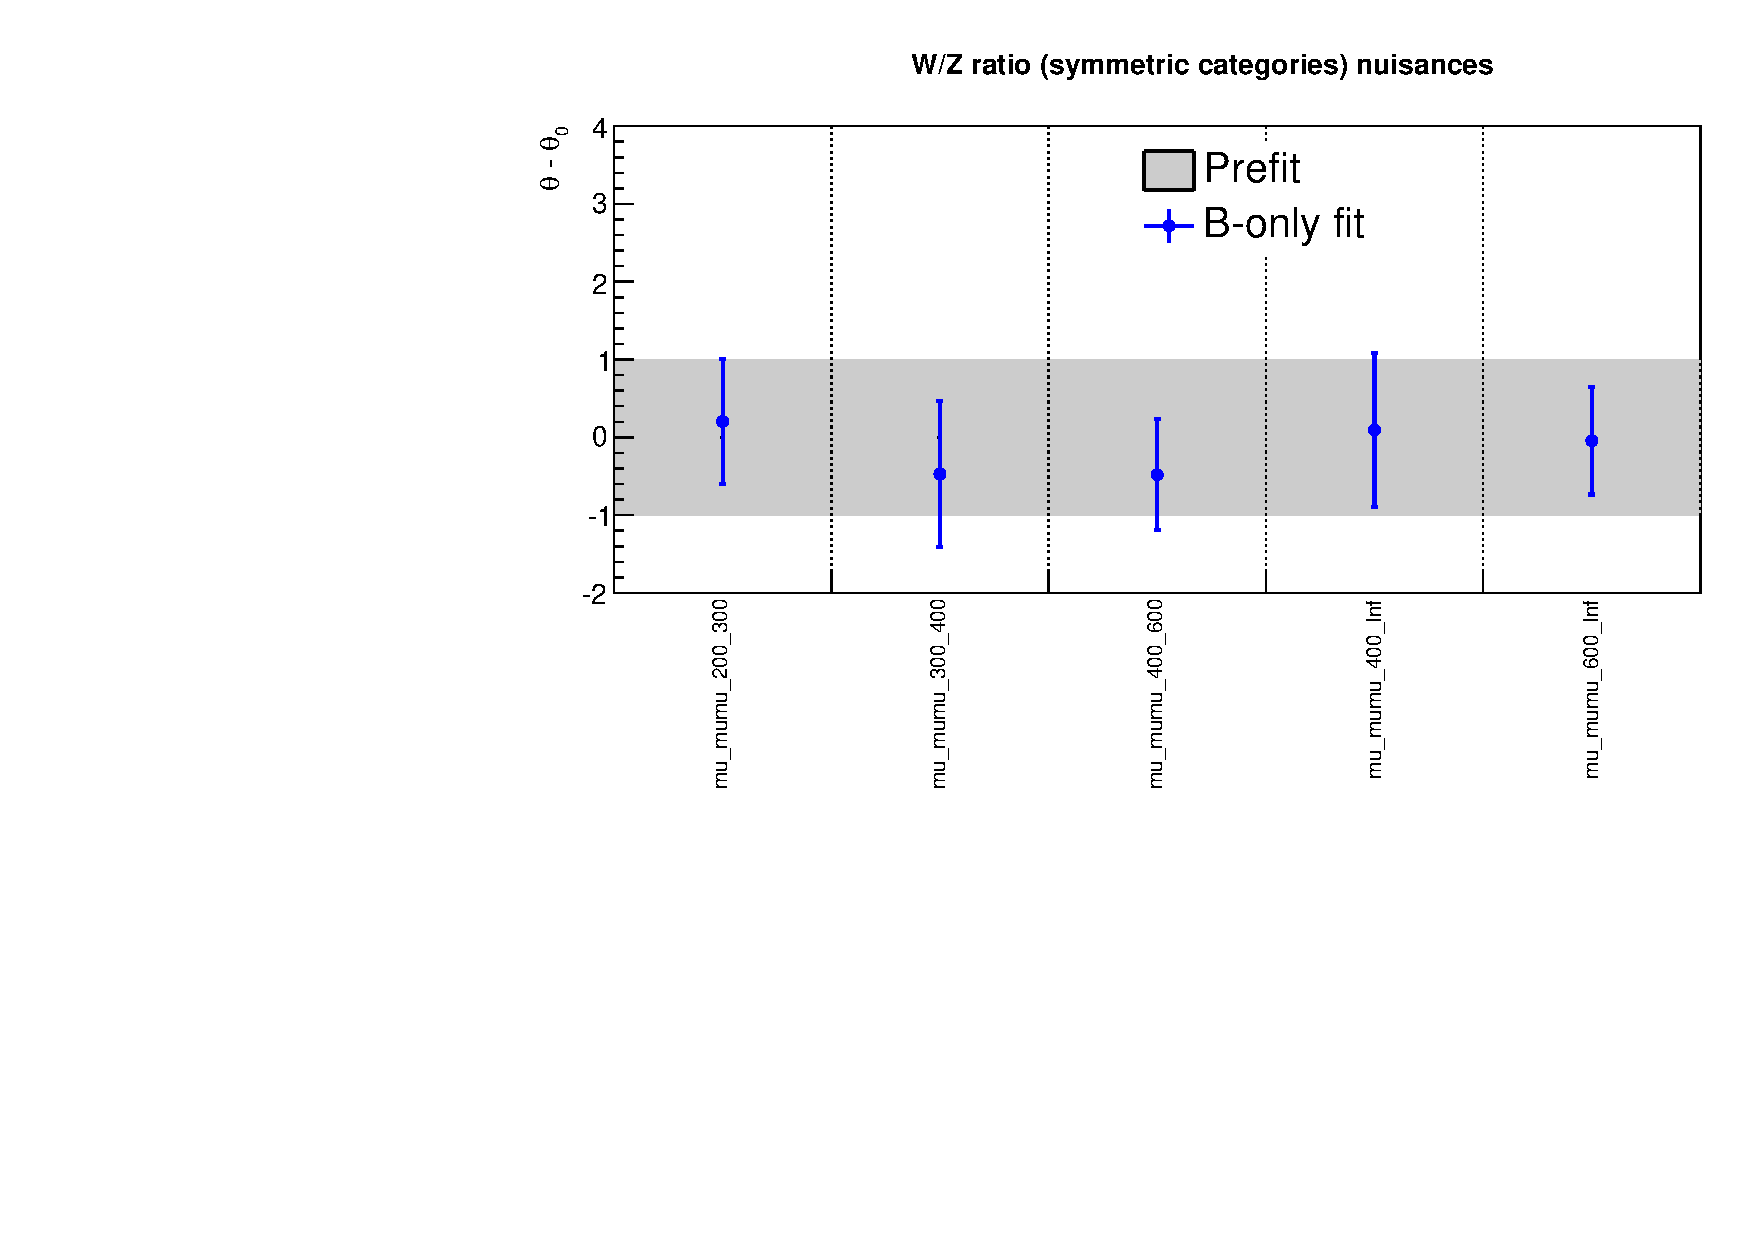
\includegraphics[width=0.45\textwidth]{AN-15-004/trunk/figures/postFitResults/nuisancePlots/W_Z_ratio_sym_nuisances} }
%  \end{center}
%\end{figure}


%\begin{figure}[tbhp]
%    \caption{ Pull of the nuisances parameters associated to the $\ttbar/W$ admixture systematic uncertainty, 
%      for the asymmetric (symmetric) categories on the left (right).
%      \label{fig:nuisPull_tt_W_admixture}}
%  \begin{center}
%    \subfigure[Asymmetric categories]{ 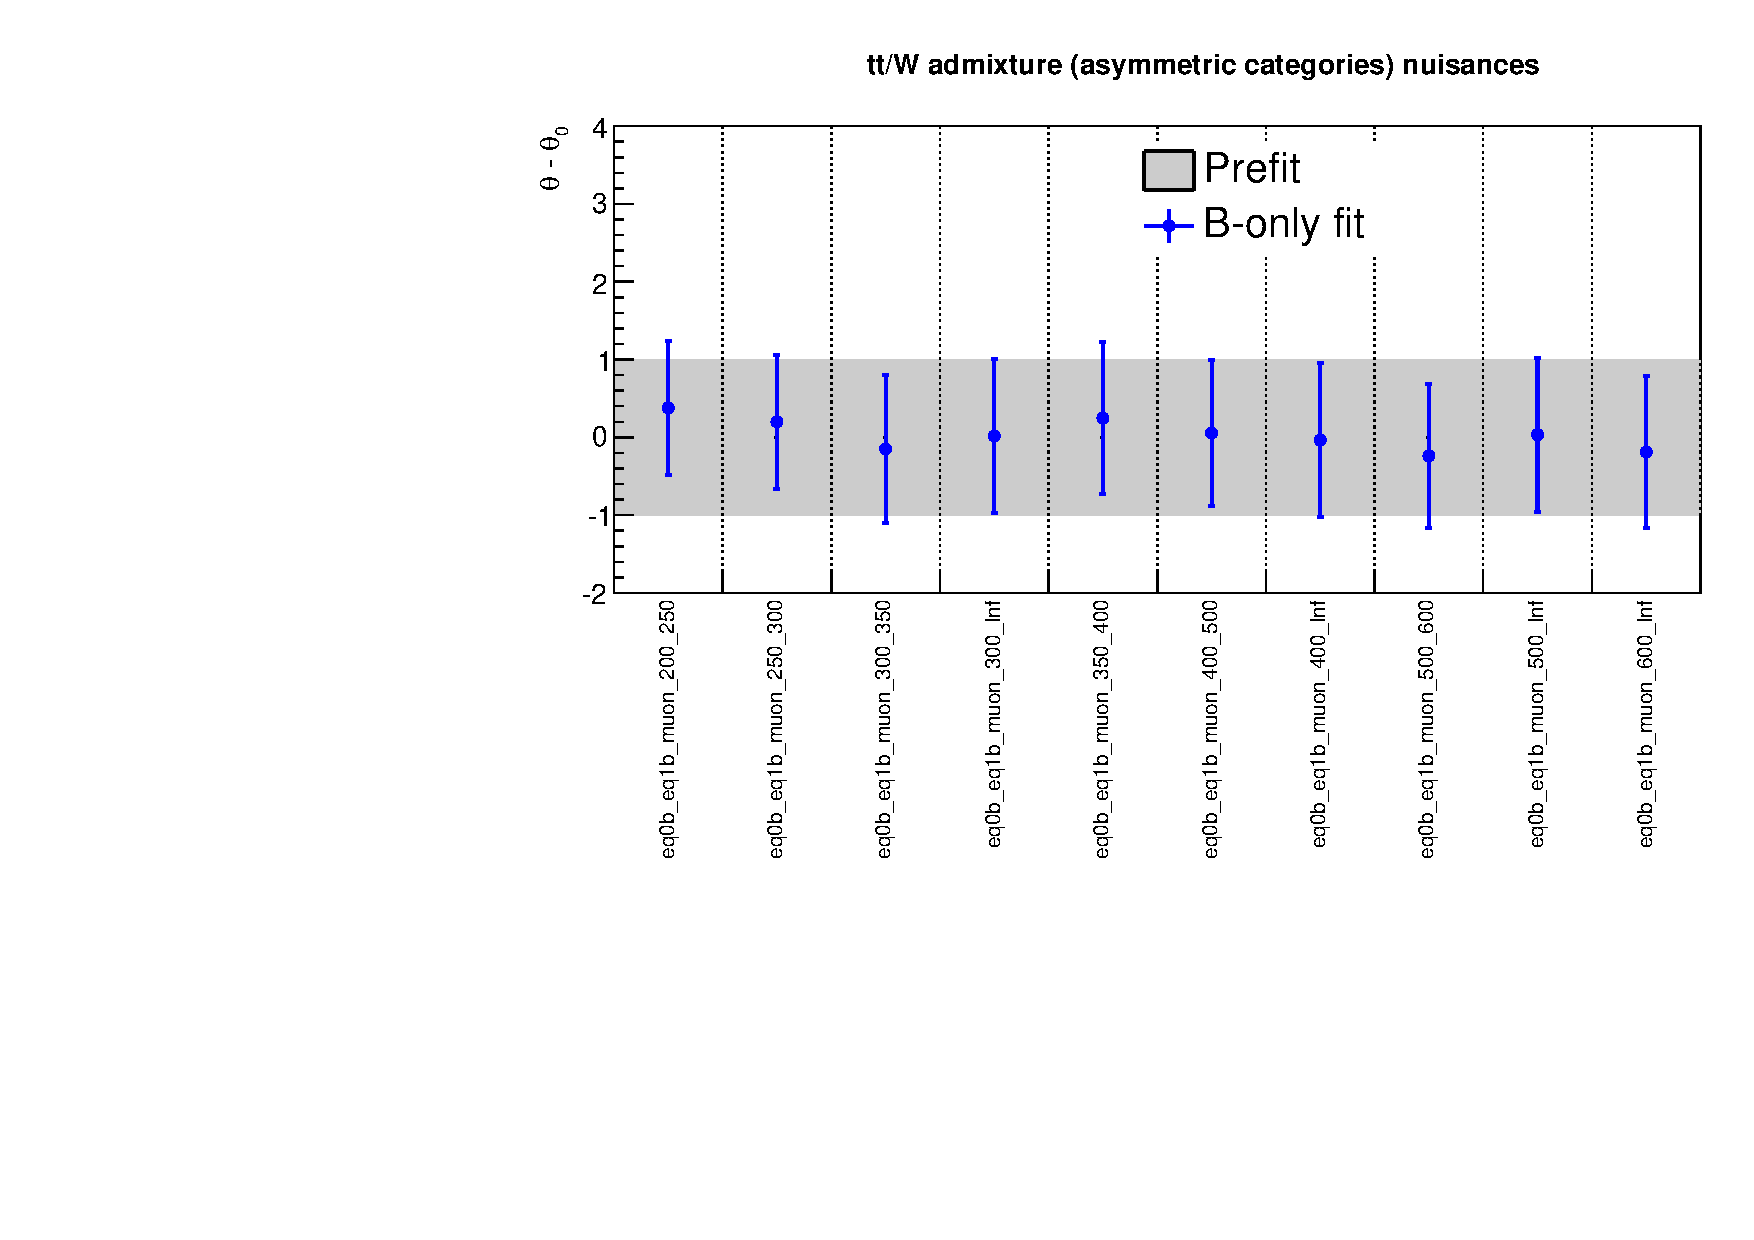
\includegraphics[width=0.45\textwidth]{AN-15-004/trunk/figures/postFitResults/nuisancePlots/tt_W_admixture_asym_nuisances} } ~~
%    \subfigure[Symmetric categories]{ 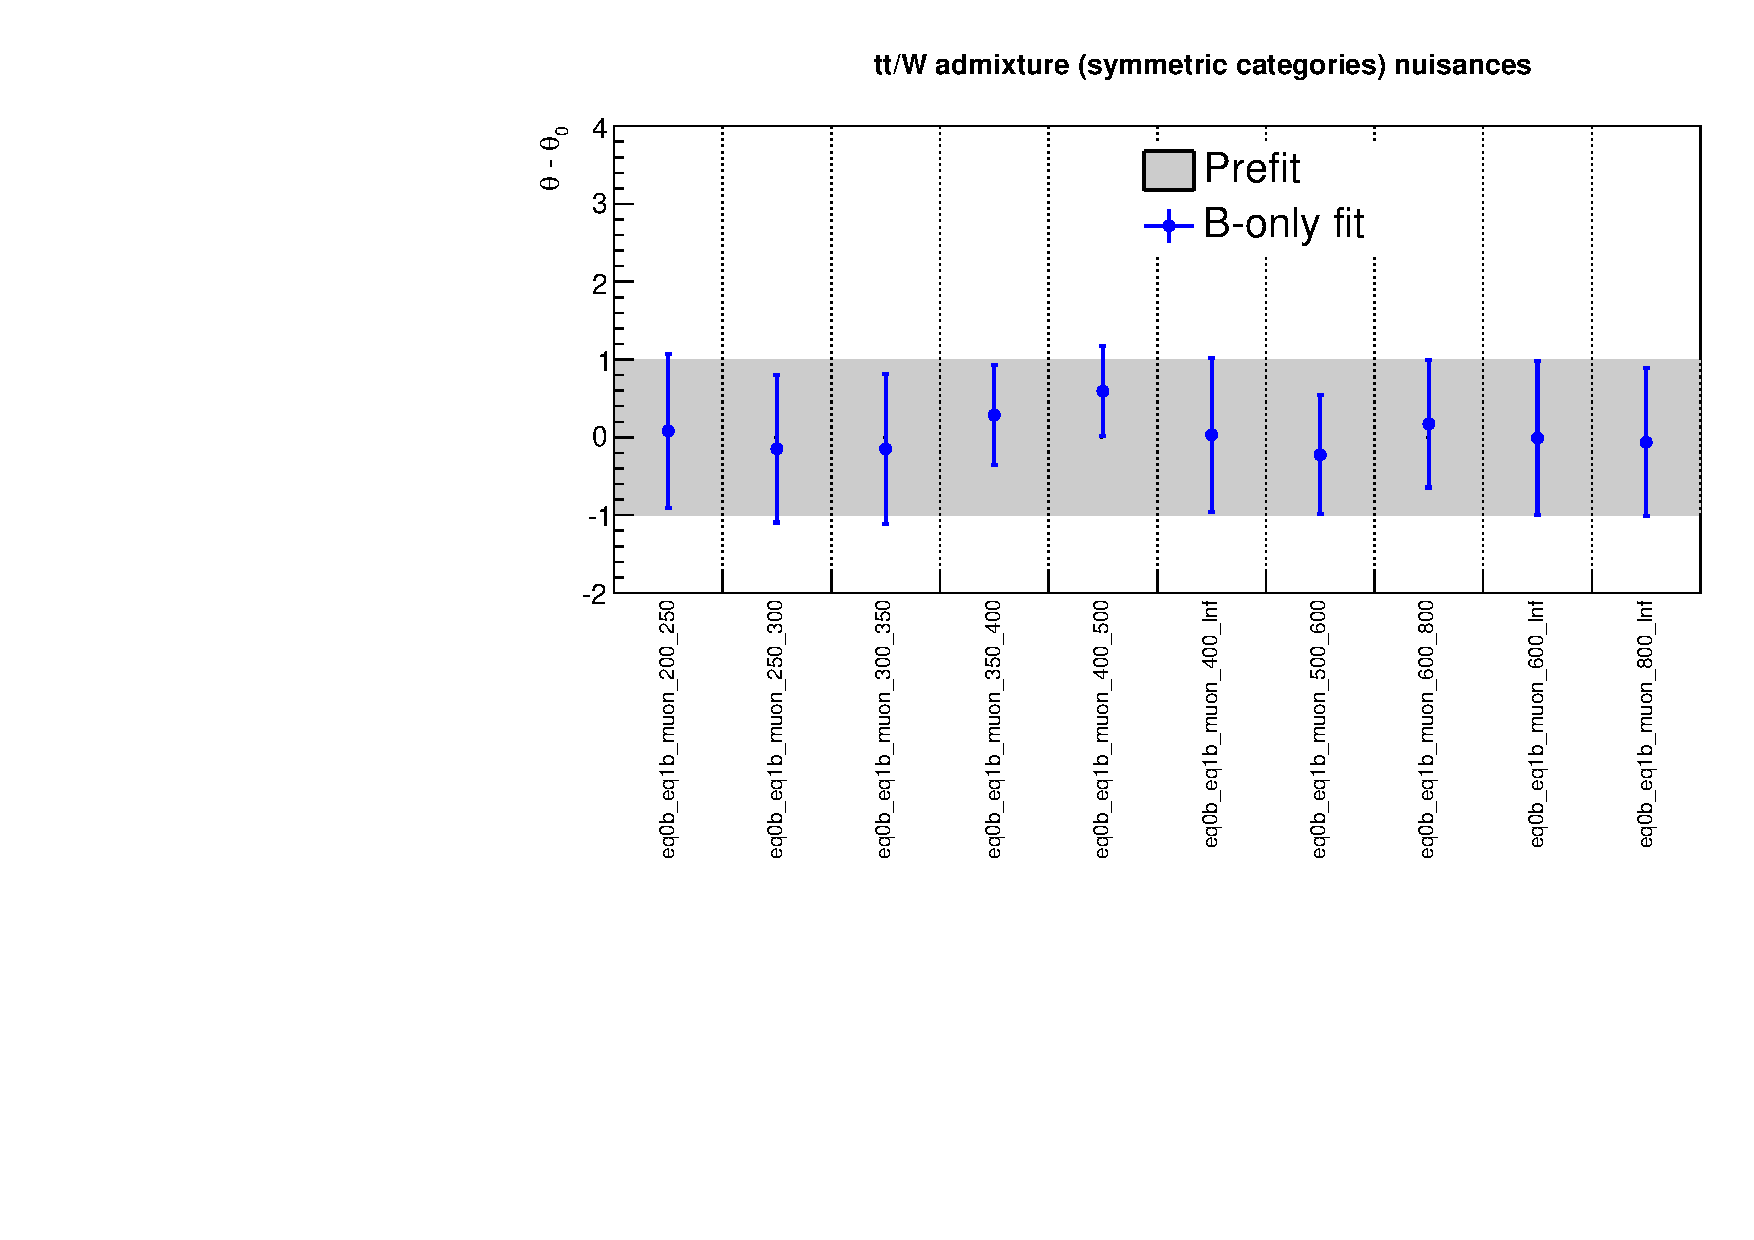
\includegraphics[width=0.45\textwidth]{AN-15-004/trunk/figures/postFitResults/nuisancePlots/tt_W_admixture_sym_nuisances} }
%  \end{center}
%\end{figure}


%\begin{figure}[tbhp]
%    \caption{ Pull of the nuisances parameters associated to the W polarisation systematic uncertainty, 
%      for the asymmetric (symmetric) categories on the left (right).
%      \label{fig:nuisPull_WPol}}
%  \begin{center}
%    \subfigure[Asymmetric categories]{ 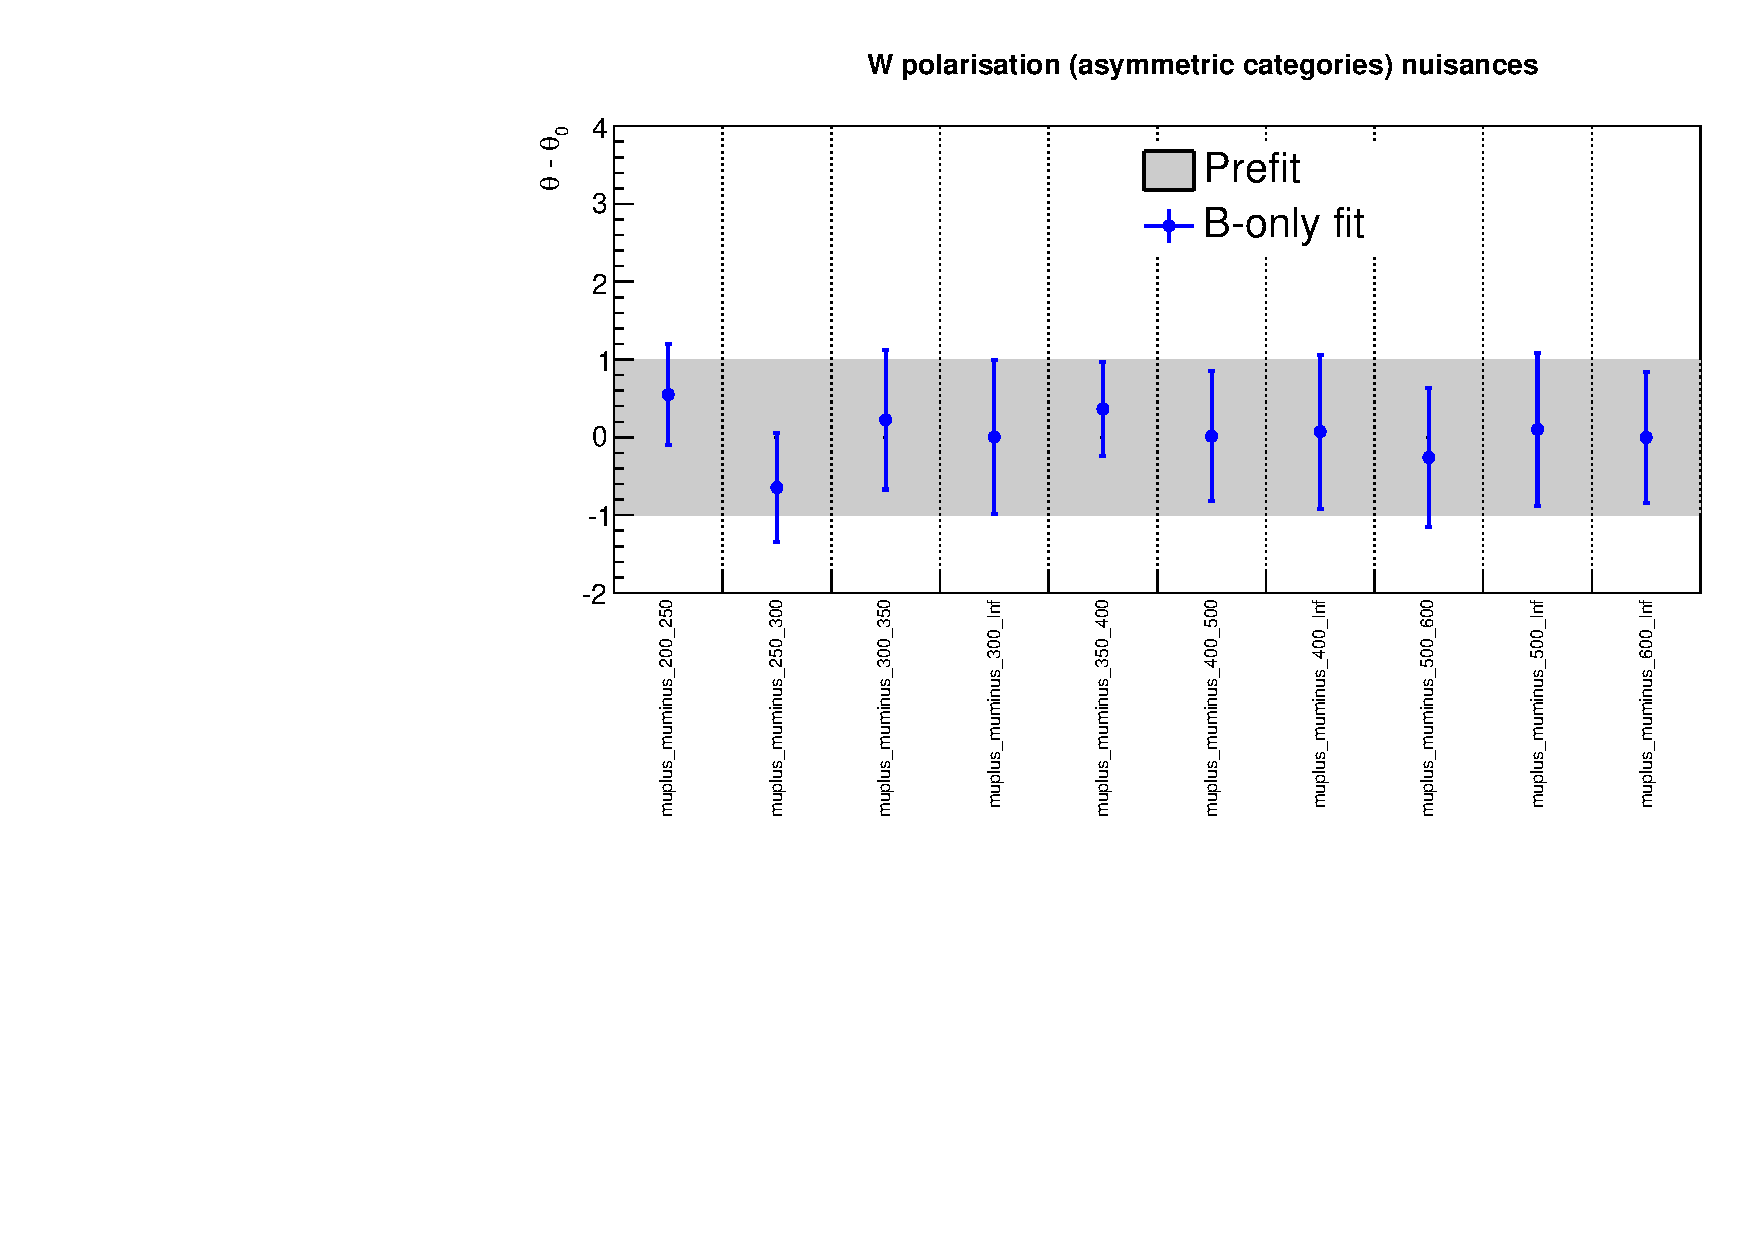
\includegraphics[width=0.45\textwidth]{AN-15-004/trunk/figures/postFitResults/nuisancePlots/WPol_asym_nuisances} } ~~
%    \subfigure[Symmetric categories]{ 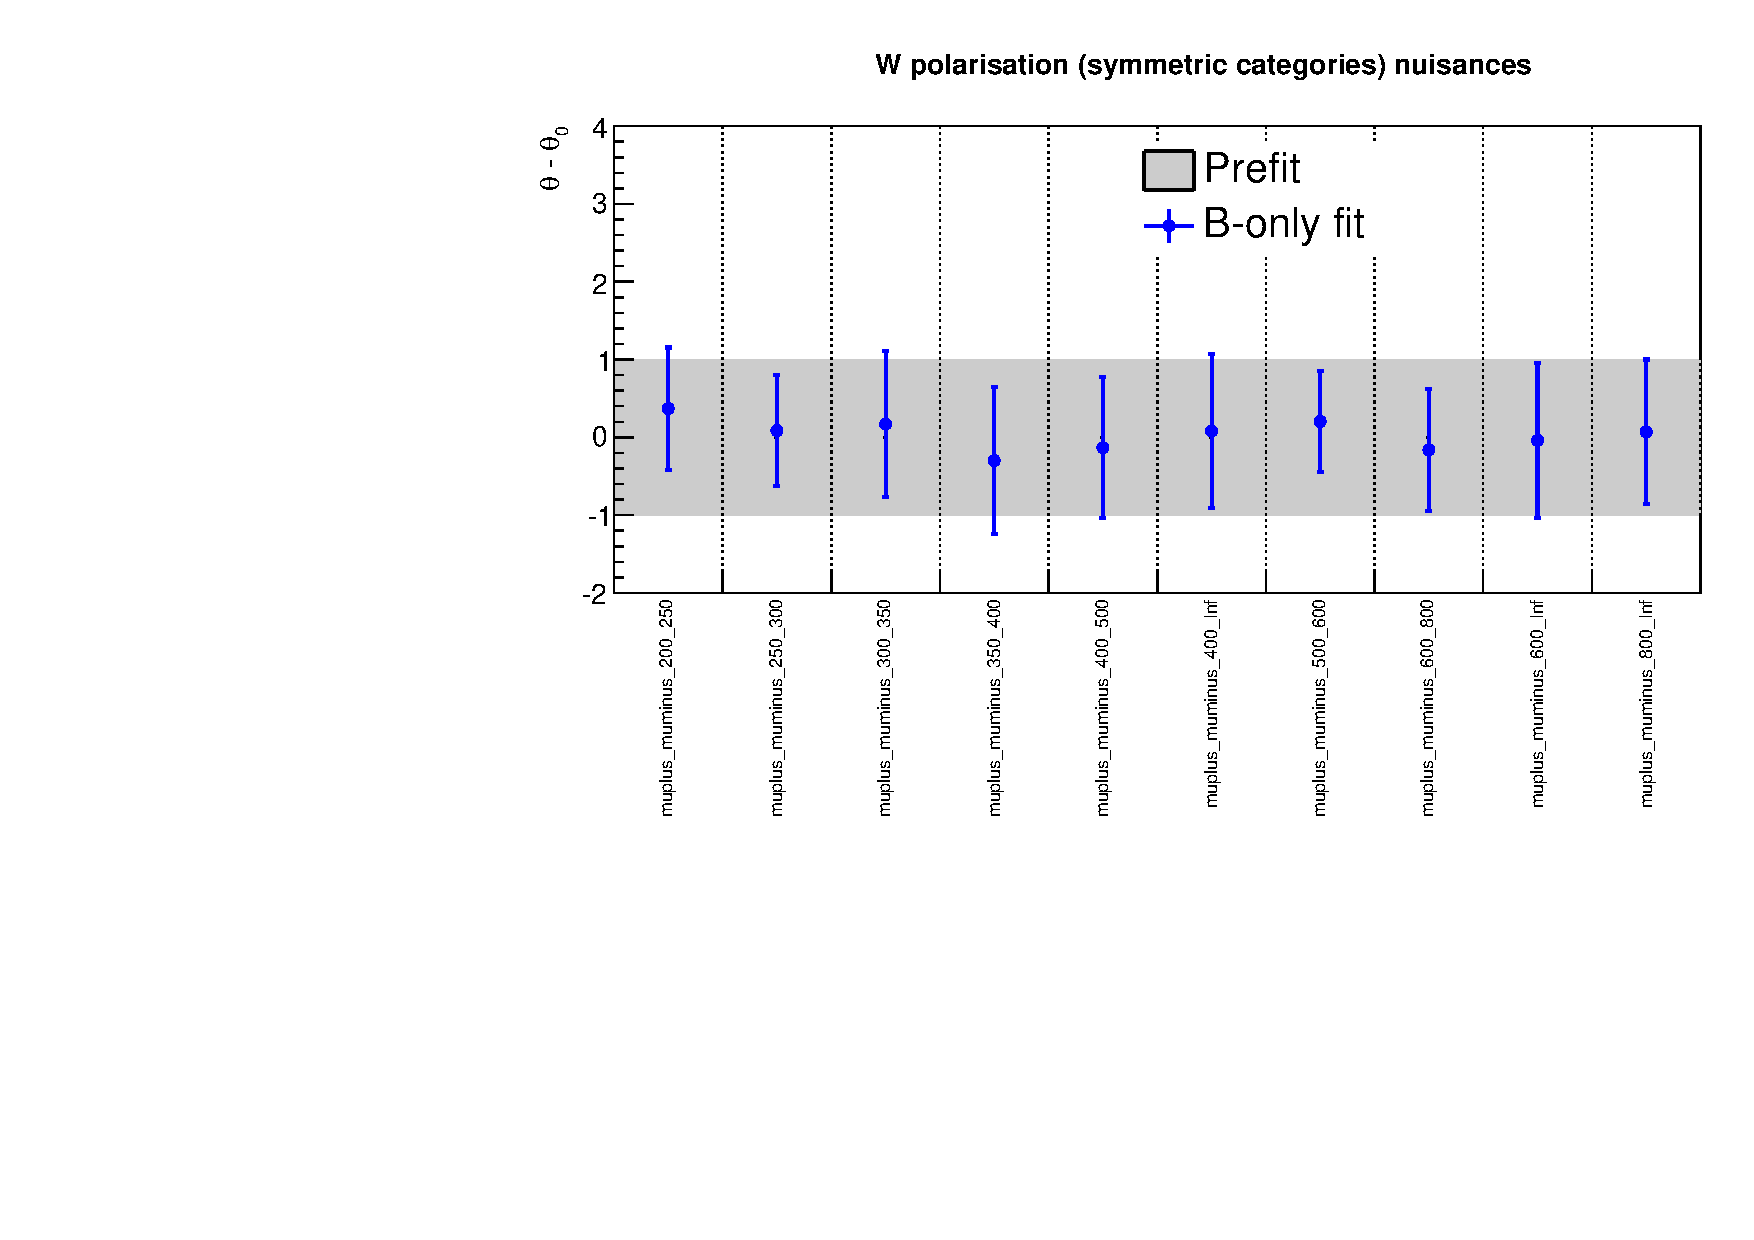
\includegraphics[width=0.45\textwidth]{AN-15-004/trunk/figures/postFitResults/nuisancePlots/WPol_sym_nuisances} }
%  \end{center}
%\end{figure}
%
%
%\begin{figure}[tbhp]
%    \caption{ Pull of the nuisances parameters associated to the $\ttbar+W$ template systematic uncertainty, 
%      for the asymmetric (symmetric) categories on the left (right).
%      \label{fig:nuisPull_TemplateTtw}}
%  \begin{center}
%    \subfigure[Asymmetric categories]{ 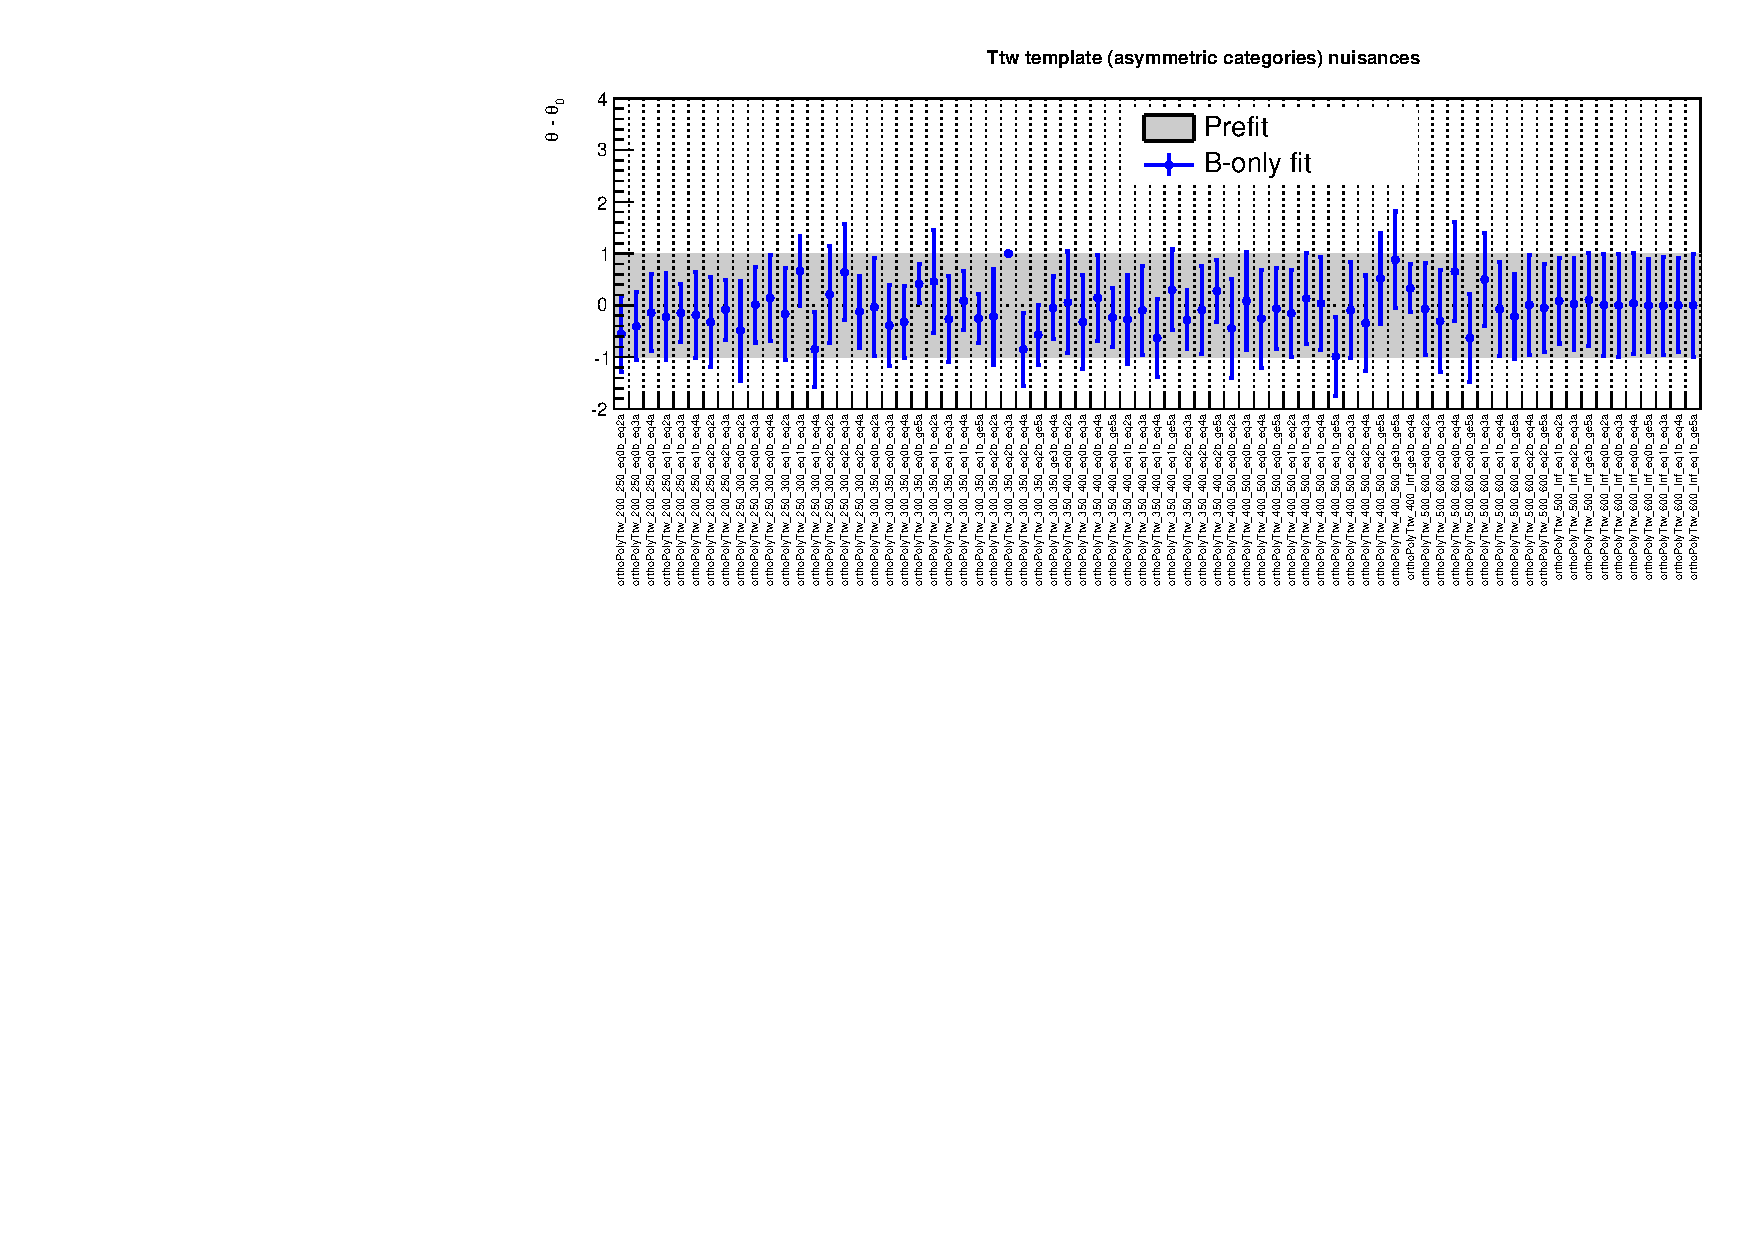
\includegraphics[width=0.8\textwidth]{AN-15-004/trunk/figures/postFitResults/nuisancePlots/TemplateTtw_asym_nuisances} } \\
%    \subfigure[Symmetric categories]{ 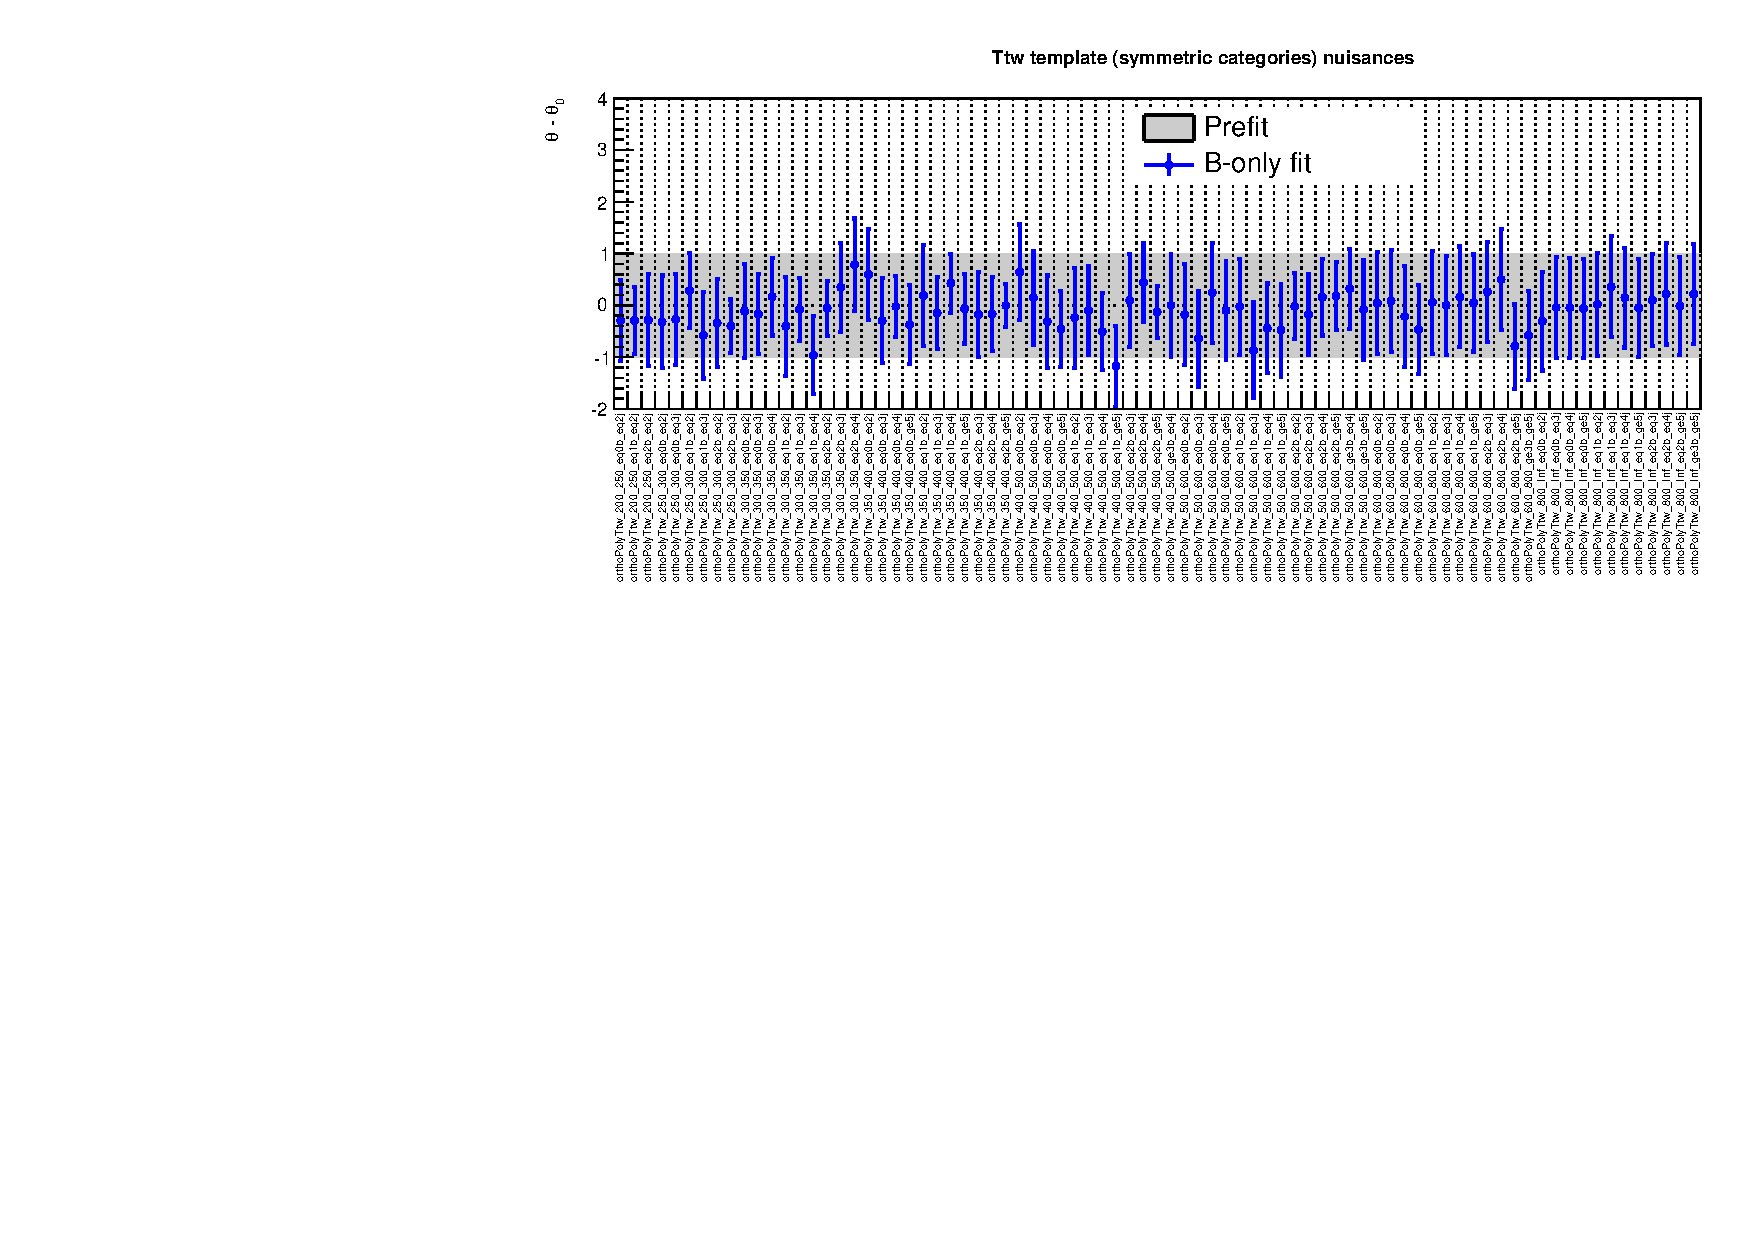
\includegraphics[width=0.8\textwidth]{AN-15-004/trunk/figures/postFitResults/nuisancePlots/TemplateTtw_sym_nuisances} }
%  \end{center}
%\end{figure}
%
%
%\begin{figure}[tbhp]
%    \caption{ Pull of the nuisances parameters associated to the $\ttbar+W$ template systematic uncertainty, 
%      for the asymmetric (symmetric) categories on the left (right).
%      \label{fig:nuisPull_TemplateZinv}}
%  \begin{center}
%    \subfigure[Asymmetric categories]{ 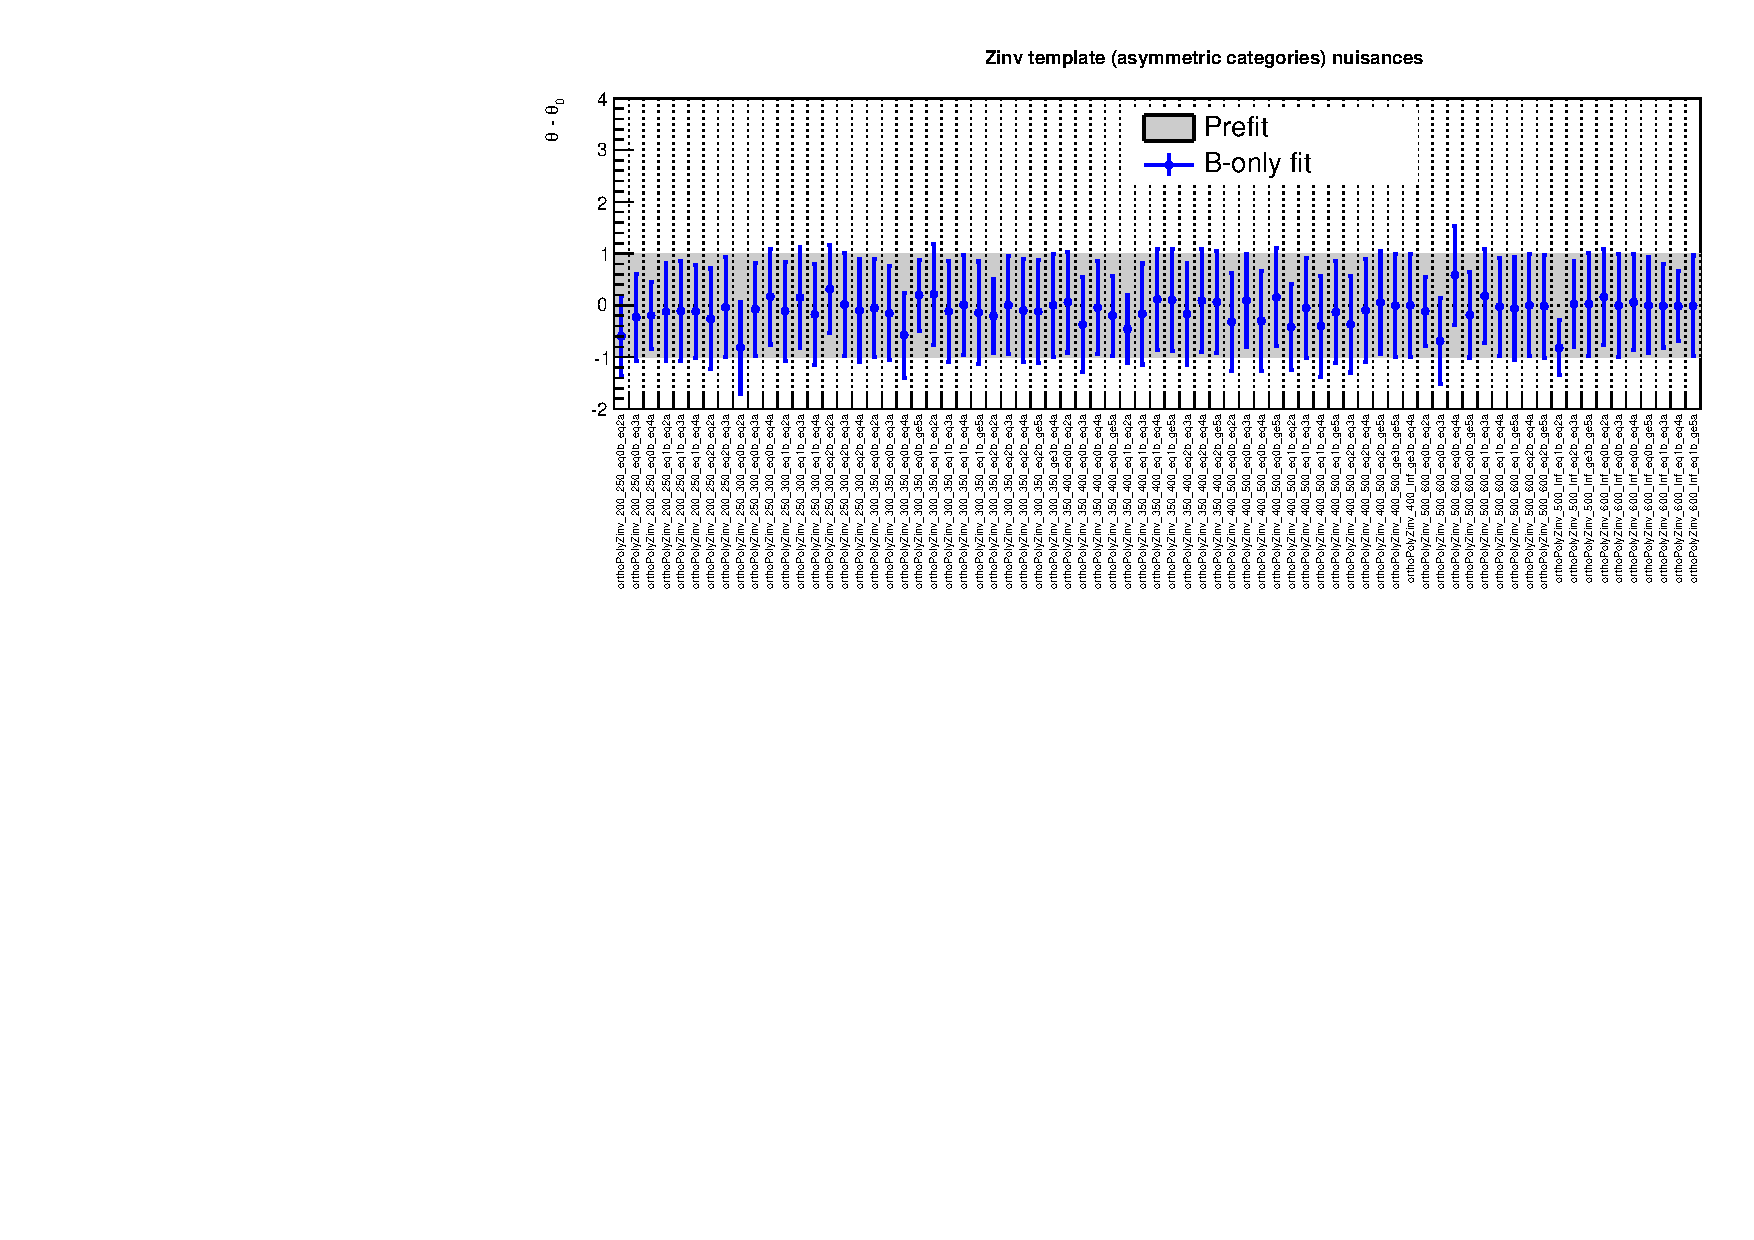
\includegraphics[width=0.8\textwidth]{AN-15-004/trunk/figures/postFitResults/nuisancePlots/TemplateZinv_asym_nuisances} } \\
%    \subfigure[Symmetric categories]{ 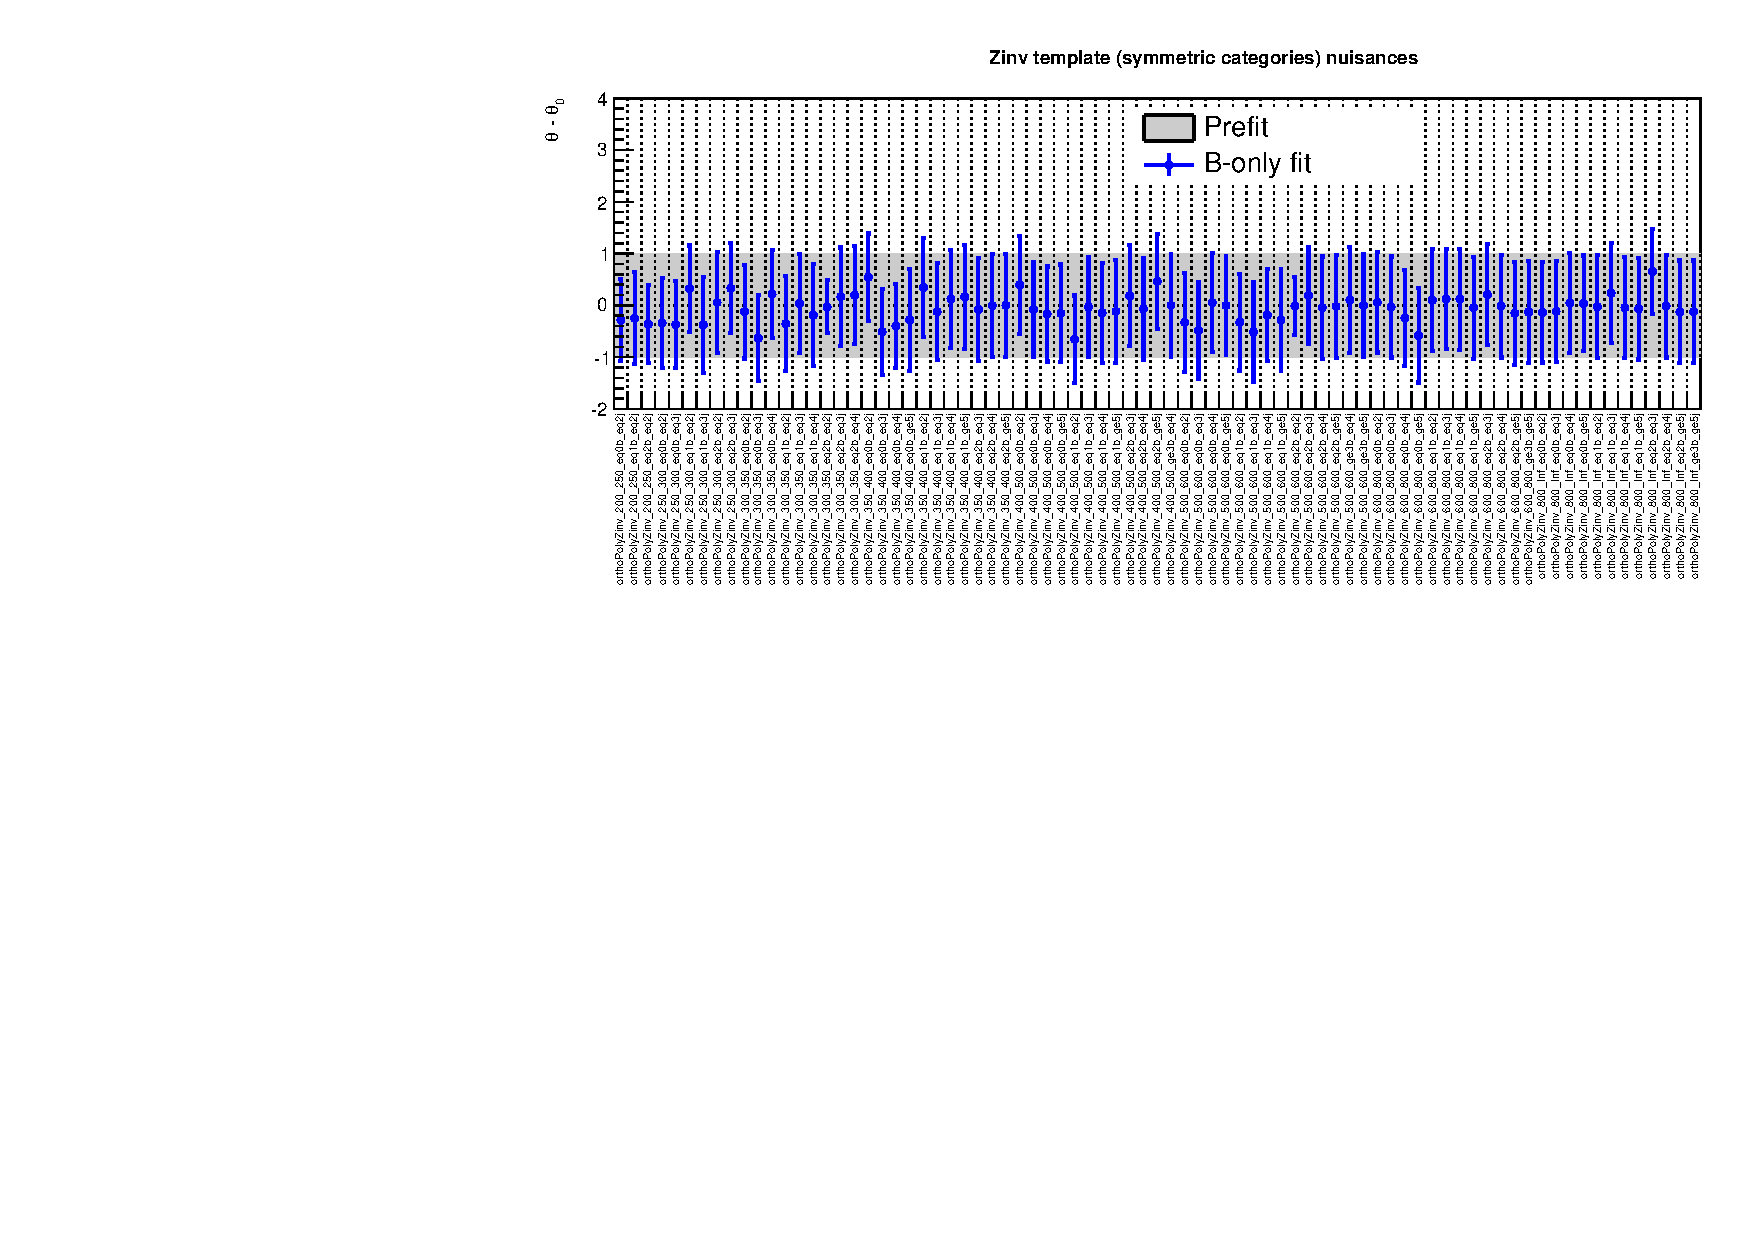
\includegraphics[width=0.8\textwidth]{AN-15-004/trunk/figures/postFitResults/nuisancePlots/TemplateZinv_sym_nuisances} }
%  \end{center}
%\end{figure}
%
%
%\begin{figure}[tbhp]
%    \caption{ Pull of the nuisances parameters associated to the QCD systematic uncertainty, 
%      for the asymmetric (symmetric) categories on the left (right).
%      \label{fig:nuisPull_qcd}}
%  \begin{center}
%    \subfigure[Asymmetric categories]{ 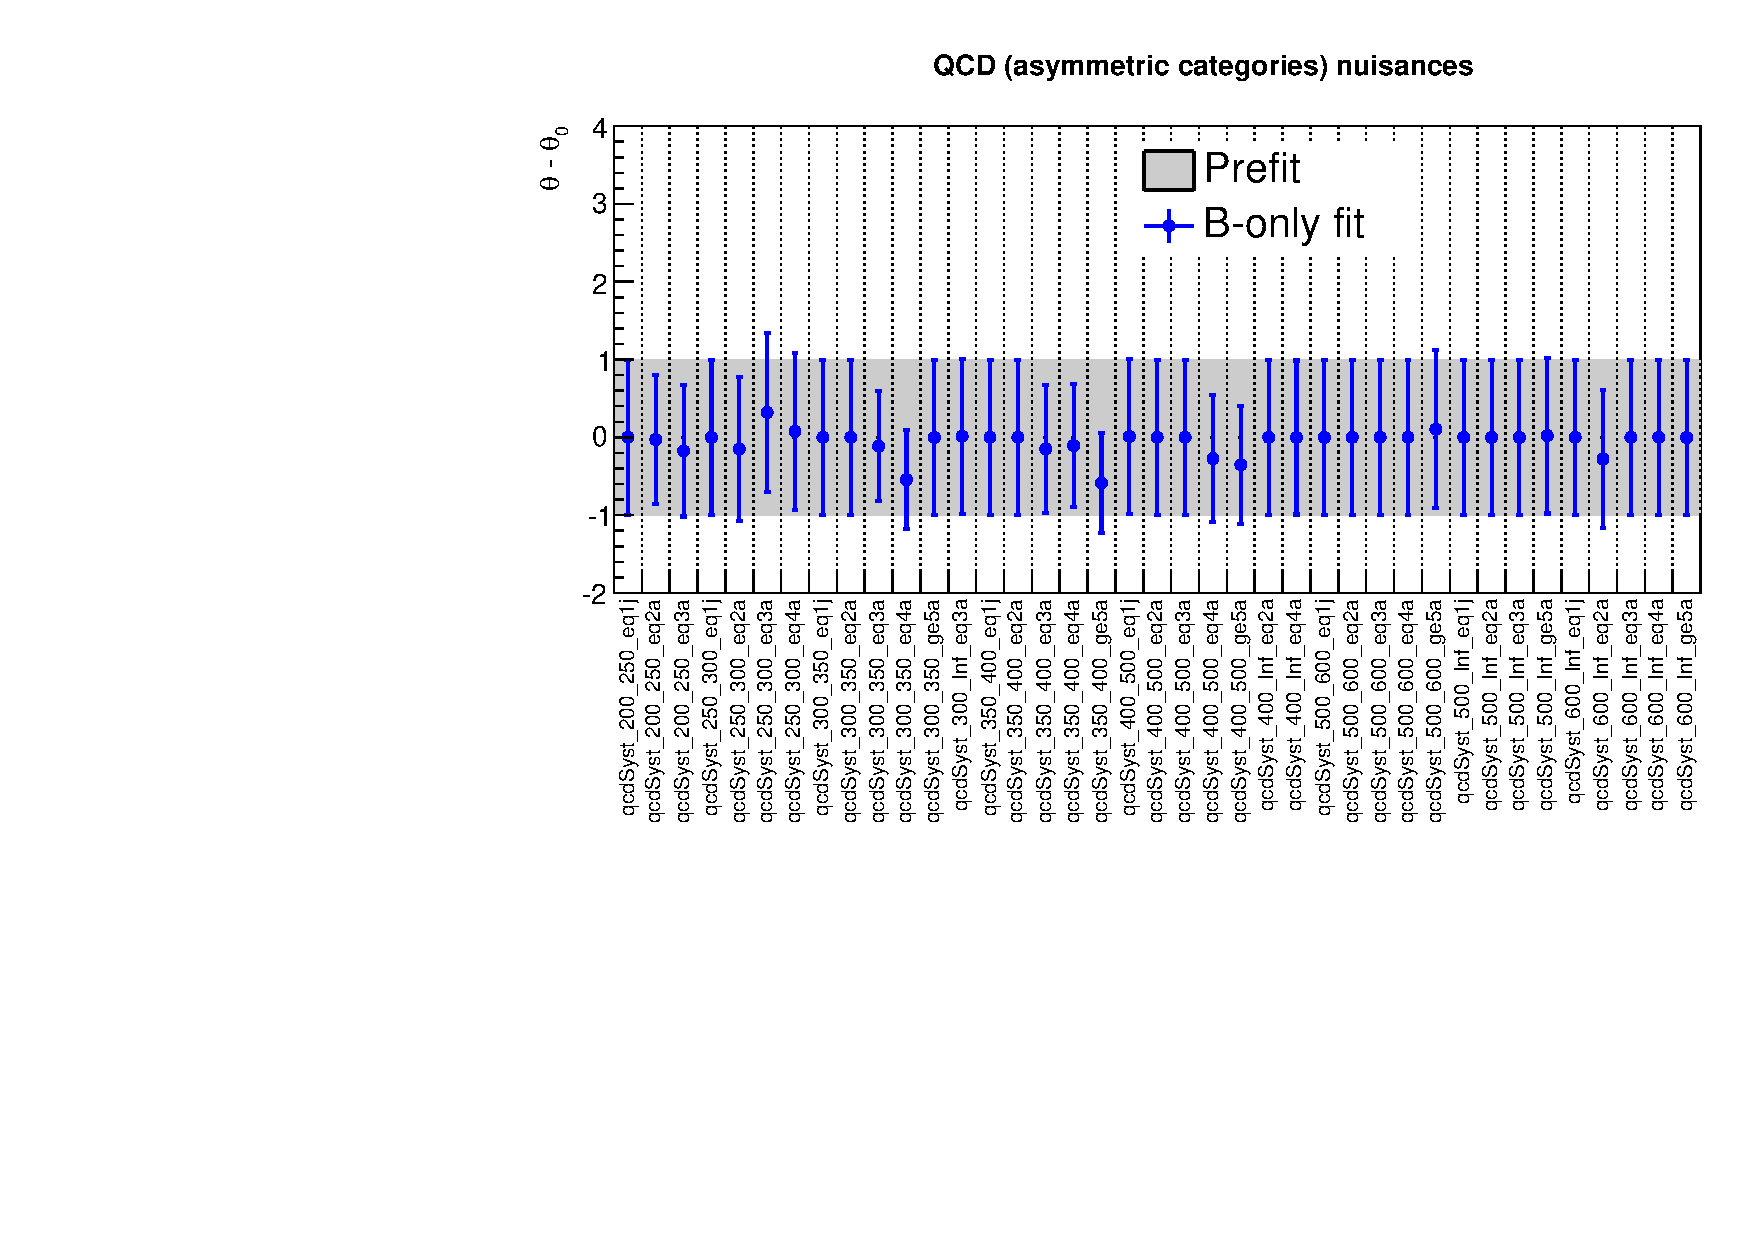
\includegraphics[width=0.45\textwidth]{AN-15-004/trunk/figures/postFitResults/nuisancePlots/qcd_asym_nuisances} } ~~
%    \subfigure[Symmetric categories]{ 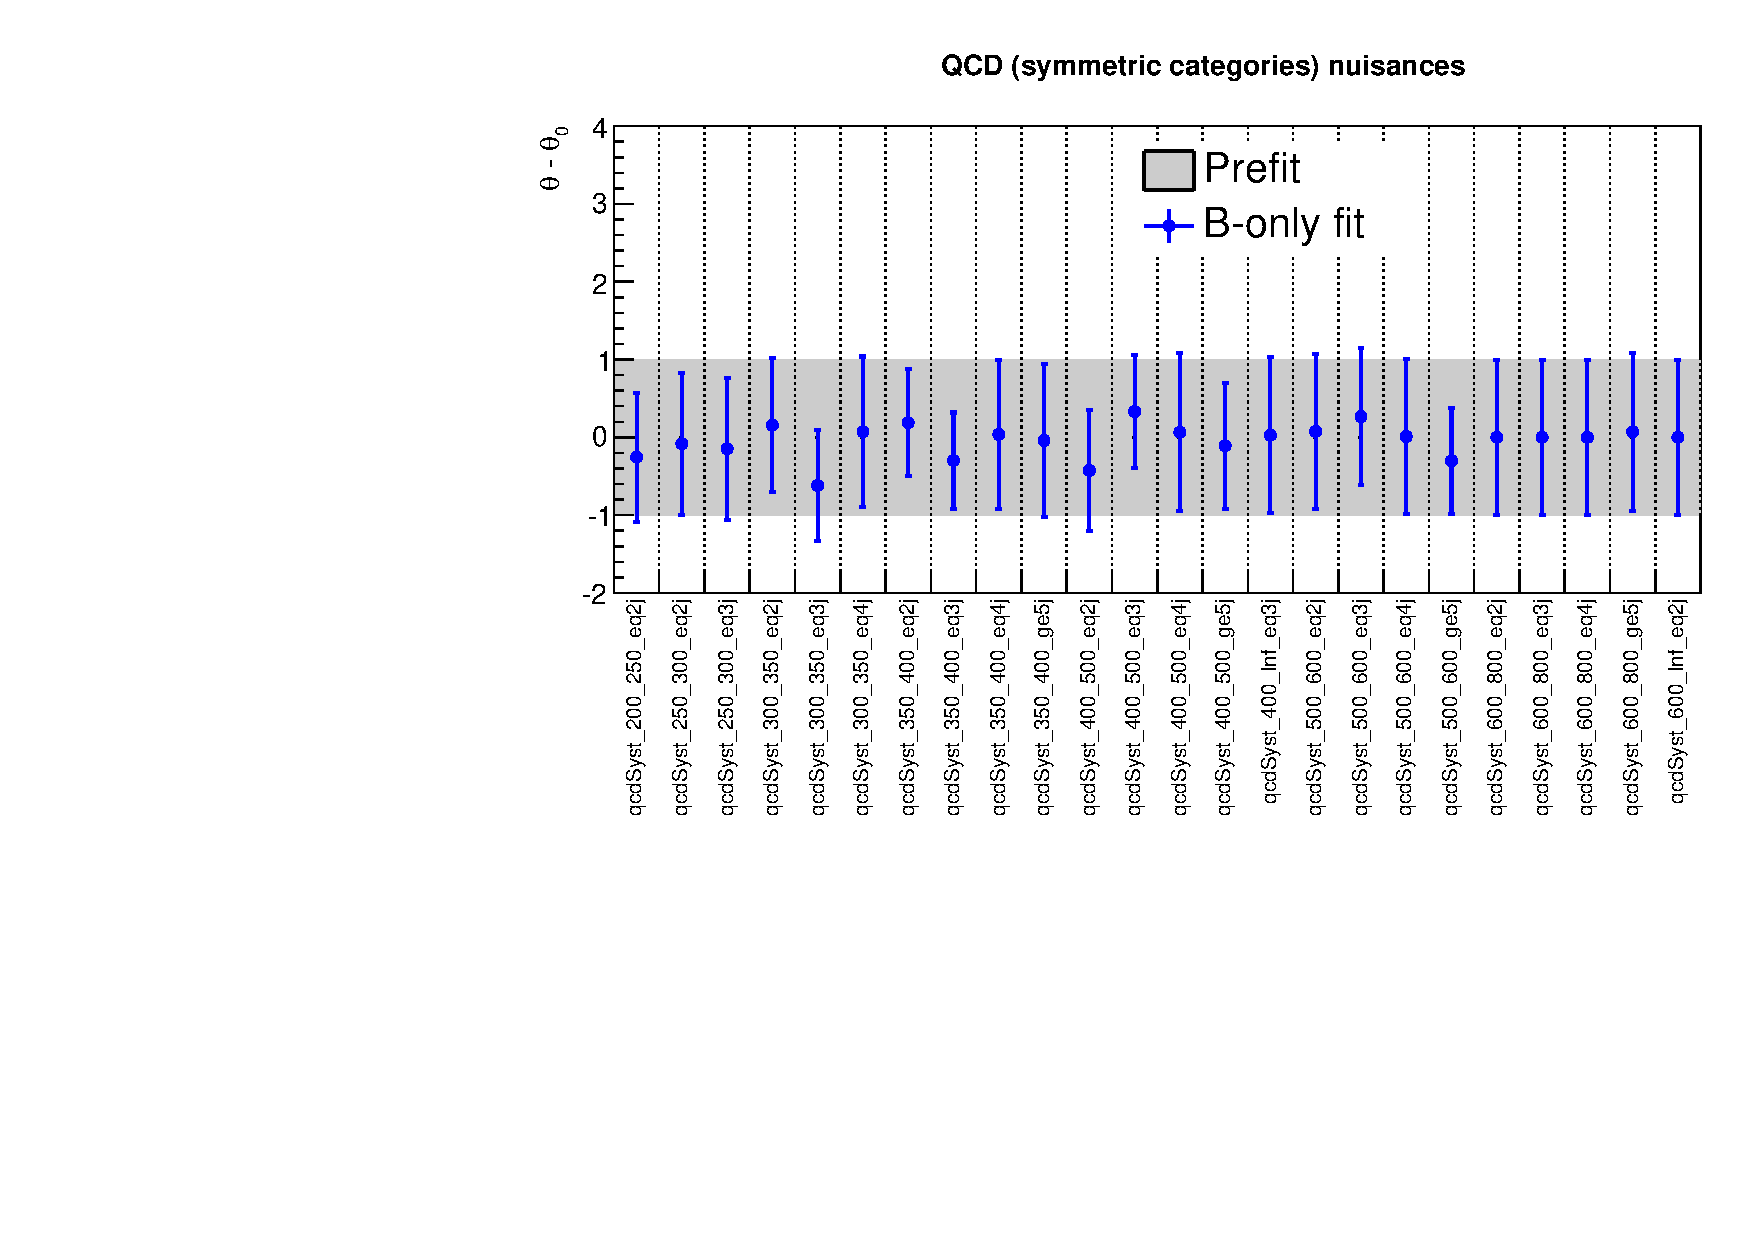
\includegraphics[width=0.45\textwidth]{AN-15-004/trunk/figures/postFitResults/nuisancePlots/qcd_sym_nuisances} }
%  \end{center}
%\end{figure}
%
%
%\begin{figure}[tbhp]
%    \caption{ Pull of the nuisances parameters associated to the correlated systematic uncertainties. 
%      \label{fig:nuisPull_Correlated}}
%  \begin{center}
%    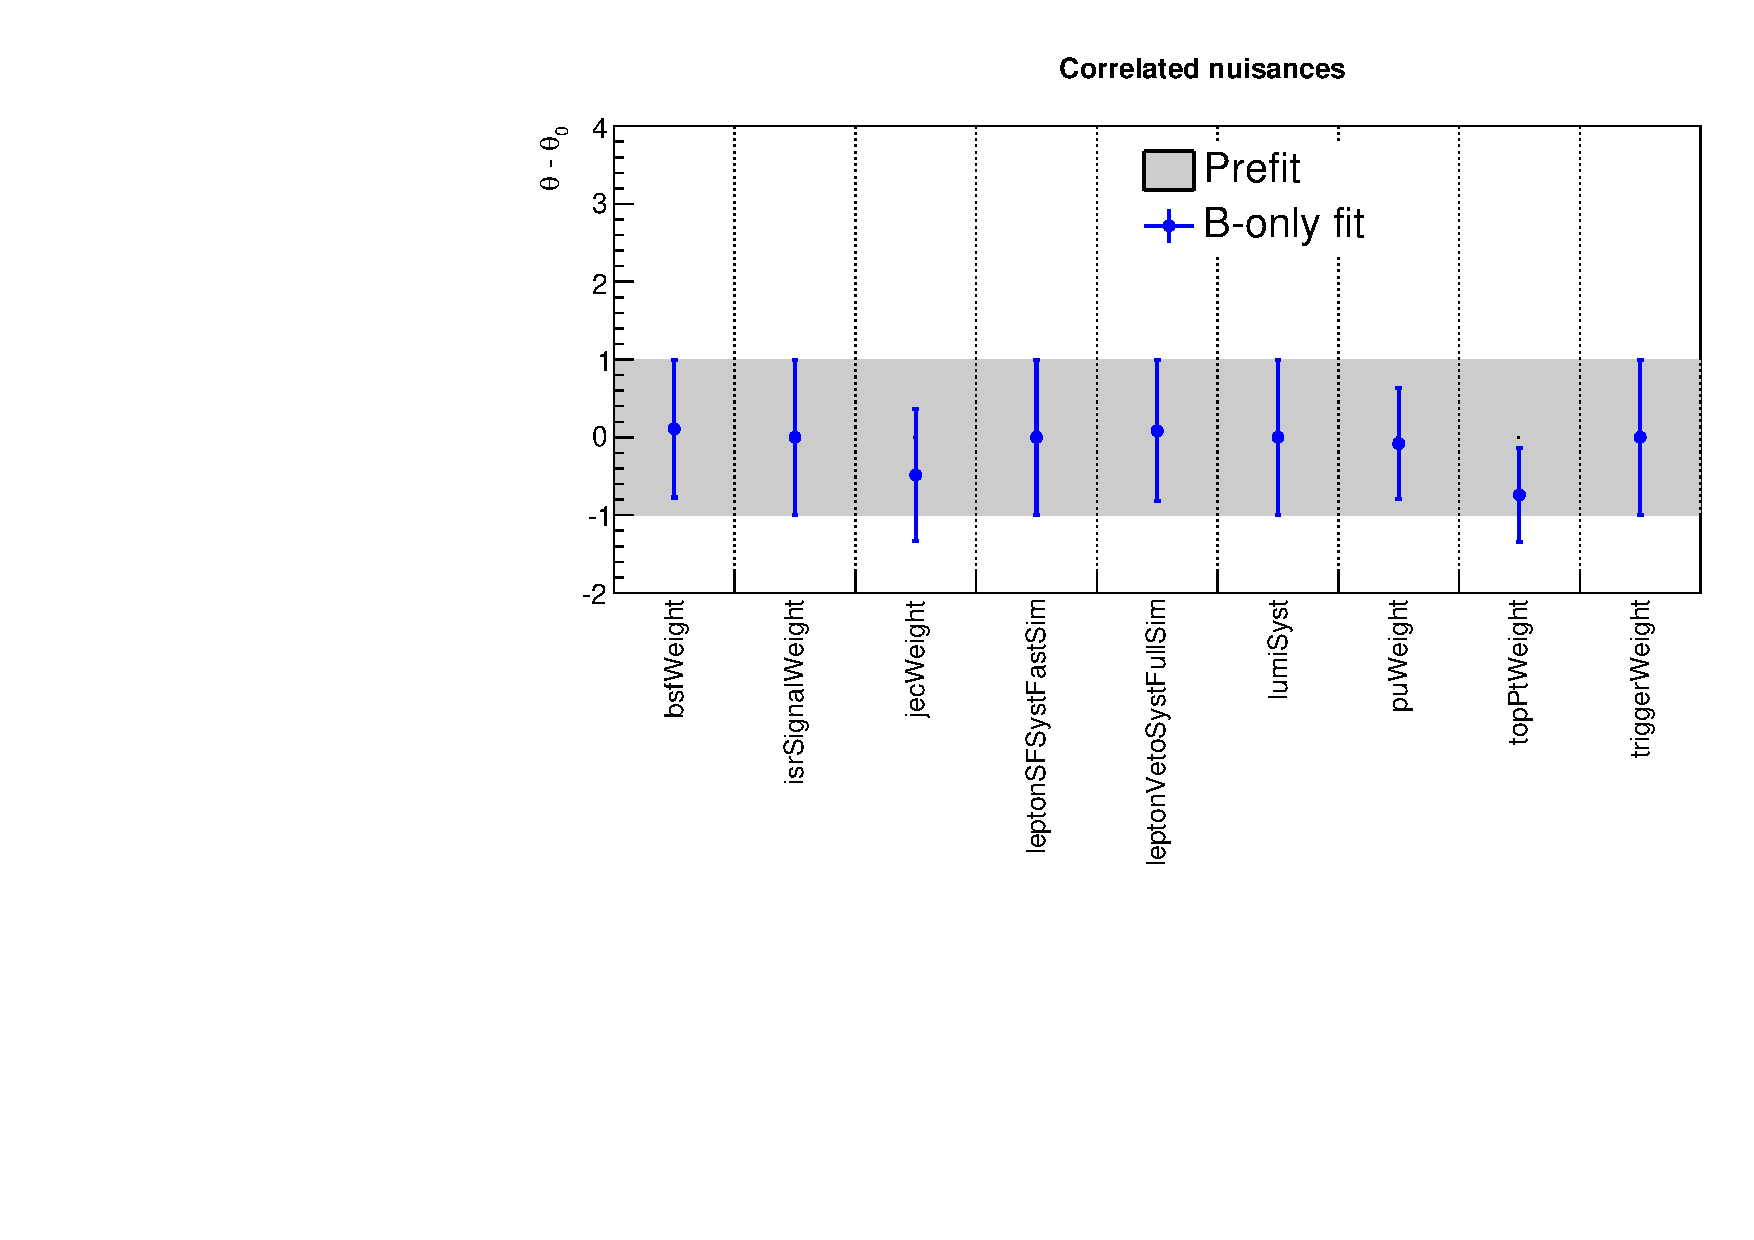
\includegraphics[width=0.8\textwidth]{AN-15-004/trunk/figures/postFitResults/nuisancePlots/Correlated_nuisances}
%  \end{center}
%\end{figure}


Section 15 in Ref.~\cite{alphaTnote} also presents the pull distributions of the nuisance parameters from systematic uncertainties and transfer factors.
